\providecommand{\g}[1]{\textcolor{purple}{[#1]}}
\providecommand{\toedit}[1]{\textcolor{teal}{\textbf{[to edit:} #1\textbf{]}}}
\newcommand{\exptable}[1]{{\vspace*{0.5em}\footnotesize\setlength{\tabcolsep}{4pt}\resizebox{\ifdim\width>\linewidth\linewidth\else\width\fi}{!}{\input{tables/#1}}}}

\FloatBarrier
\section{Experimental methods}
\label{app:experiments}
The experiments start from the MNIST baseline in Appendix~\ref{app:protocol}. Each comparison below states what changes, which parameters are measured, and how the resulting spaces are checked. Results follow in Appendices~\ref{app:theoretical-support}--\ref{app:additional-material}.

\paragraph{Computing infrastructure.}\label{app:compute}
Experiments used a shared Linux server with two AMD EPYC 9554 processors (128 physical cores, 256 hardware threads), approximately 377\,GiB of host memory and four NVIDIA RTX A6000 GPUs with 48\,GB each. Training and network evaluation used GPUs; dense Jacobian factorizations also used CPU linear algebra. Geometry calculations used float64, with thread limits and memory checks for large factorizations.

\paragraph{Software.}\label{app:software}
The implementation uses PyTorch \citep{paszke2019pytorch} and TorchVision \citep{torchvision}, with NumPy \citep{harris2020numpy} and SciPy \citep{virtanen2020scipy} for numerical calculations, scikit-learn \citep{pedregosa2011sklearn} for clustering comparison scores, and Matplotlib \citep{hunter2007matplotlib} for figures.

\subsection{Jacobians, SVDs and numerical validation}
\label{app:sanity}
\paragraph{Jacobians and ranks.}
We differentiate the outputs on the fixed analysis set with respect to one affine layer or the whole parameter vector. For an MLP layer, the explicit Jacobian combines each augmented input feature with its downstream derivative. For a convolutional layer, contributions from all spatial positions are summed in the shared kernel coordinates. Explicit rows are checked against automatic differentiation.

Dense Jacobians are reduced by QR, followed by an SVD of the triangular factor. This avoids squaring the condition number by forming a Gram matrix. The same rank rule is applied to feature and downstream matrices to obtain the atomic decomposition.

For the largest layers, storing and factorizing the full Jacobian is too expensive. We instead estimate its range by randomized subspace iteration, using products with the Jacobian. Write $J\in\R^{sd\times p_\ell}$, where $s$ is the number of analysis samples, $d$ the output dimension and $p_\ell$ the number of parameters in the edited layer. We draw $k$ Gaussian parameter directions as columns of $\Omega\in\R^{p_\ell\times k}$ and compute
\[
 Y=J\Omega,\qquad Q=\operatorname{orth}(Y),\qquad B=Q^\top J.
\]
Here $\operatorname{orth}$ returns an orthonormal basis, and $k$ is the number of sampled directions. Products with $J$ and $J^\top$ are evaluated in chunks, without storing the full Jacobian. Repeated products refine $Q$; the singular values of the smaller matrix $B$ estimate the resolved spectrum. The residual $\|(I-QQ^\top)J\|_{\rm op}$ measures what lies outside the recovered image. Its numerical upper estimate is checked against the rank threshold before reporting a resolved rank. If the allowed value of $k$ is exhausted first, only a rank lower bound is reported. We use two subspace iterations with QR after each multiplication and double the sketch size from $k=32$ up to the memory cap (8,192 for the width-512 hidden layers); a full-dimension sketch uses no power iteration. Six fresh Gaussian probes $g_a$ give the omitted-range bound $\eta=10\sqrt{2/\pi}\max_{a\le6}\|(I-QQ^\top)Jg_a\|_2$ with failure probability at most $10^{-6}$ per check \citep[Lemma 4.1]{halko2011randomized}; rank $r$ is resolved only if $\hat\sigma_r>10^{-9}(\hat\sigma_1+\eta)$ and $\hat\sigma_{r+1}+\eta\le10^{-9}\hat\sigma_1$, including a $10^{-14}\hat\sigma_1$ rounding allowance in $\eta$ and a union bound over checks.

\begin{table}[!htbp]\centering
\caption{Numerical conventions. Additional construction cutoffs and unresolved ranks are stated with the affected results.}\label{tab:early-method-numerical}
\small
\begin{tabular}{p{.28\linewidth}p{.65\linewidth}}\toprule
Quantity & Convention\\\midrule
Analysis precision & Float64; stored bases checked for orthonormality and Jacobian residuals.\\
Rank & Singular values above $10^{-9}\sigma_1$, with checks at $10^{-6}\sigma_1$ and $10^{-12}\sigma_1$; $\sigma_1$ is the largest singular value.\\
Output norm & $\|V\|_X^2=s^{-1}\sum_i\|v_i\|_2^2$ for stacked outputs $V=(v_i)_{i=1}^s$; Jacobians normalized by $1/\sqrt{s}$.\\
Invariant subspace validation & Received-space constraints and frozen-polynomial residual, tolerance $10^{-9}$.\\
Output visibility & First sampled radius with $\|\Delta F_X\|_X>10^{-3}$ in activation-family scans; relative metrics for reduced-data and ViT studies are specified below.\\
Data consistency & Checkpoint, preprocessing, ordered samples and parameter coordinates matched before reusing a factor.\\\bottomrule
\end{tabular}
\end{table}

\paragraph{Gauss--Newton spectra and leading directions.}
The full-network spectrum in the motivation experiment uses the width-64 MNIST model. Its Gauss--Newton eigenvalues are proportional to the squared Jacobian singular values; a relative singular-value threshold must therefore be squared when expressed as an eigenvalue threshold. The leading three directions are recovered with a matrix-free eigensolver applying $v\mapsto J_X^\top(J_Xv)$ through automatic differentiation. We check their orthonormality, eigenpair residuals and agreement with the stored spectrum, then probe both signs of each direction. These are checkpoint-specific directions.

The reported spectral measurements concern the Jacobian and Gauss--Newton operator. For MSE, the full loss Hessian additionally contains a residual-weighted second-derivative term. That term vanishes at exact interpolation, where the Gauss--Newton operator equals the loss Hessian.

\paragraph{Validation and numerical limits.}
We check equality of the true and frozen networks at the base point, the response decomposition, and independent propagation of activation residuals. Float64 recomputation of affected stored bases removes the float32 ray floor without changing their ranks. Most ReLU and leaky-ReLU ranks are stable across the two tighter thresholds. The ReLU L3 and CNN conv5 exceptions are retained in the results, and late GELU deficiencies without a spectral gap are described as numerical kernels.

\subsection{Baseline model and training}
\label{app:protocol}
To keep the parameter dimension tractable for Jacobian factorization, the reference MNIST experiment \citep{lecunmnist} trains a biased ReLU MLP on PCA inputs. We center images using the training set, retain 256 principal components and divide by one global scale, without whitening. The same fitted transform is used for evaluation. The raw-pixel ablation checks the effect of this dimensionality reduction. Table~\ref{tab:early-method-baseline} collects the baseline settings. MSE averages over samples and output coordinates: $\mathcal L=(sd)^{-1}\sum_i\|F_i-y_i\|_2^2$.

Training and test accuracies at the analysis stages are reported for every retained ablation in Appendix~\ref{app:performance}. Each table identifies the checkpoint epochs and available seeds; an unreached milestone is left empty.

\begin{table}[!htbp]\centering
\caption{MNIST baseline. The width-64 companion uses the same training recipe and supports the full-network, invariant subspace and application analyses.}\label{tab:early-method-baseline}
\small\begin{tabular}{p{.28\linewidth}p{.65\linewidth}}\toprule
Setting & Value\\\midrule
Reference architecture & $256\to128\to128\to128\to10$, biases in every affine map.\\
Companion architecture & $256\to64\to64\to64\to10$.\\
Training data & All 60,000 training images; one-hot targets.\\
Optimization & MSE, Adam, learning rate $10^{-3}$, batch size 256, 500 epochs, no schedule.\\
Replication & Three seeds; separate initialization and minibatch-order generators.\\
Geometry data & Fixed stratified training subset $X$ of 10,000 images; disjoint comparison set $X'$ of the same size.\\\bottomrule
\end{tabular}
\end{table}

Checkpoints are selected by training quantities: initialization, early fitting, high accuracy, MSE interpolation and the late endpoint. Their thresholds and attained epochs are given in Table~\ref{tab:stages}. Test performance is reported after selection. Unreached stages remain missing rather than being replaced by the endpoint. In the reference model, the analysis set supplies more output constraints than there are parameters, so counting alone forces no kernel.

\begin{table}[!htbp]
\caption{Training-defined stages of the three reference MNIST runs. Early fitting uses training error at most $10\%$, high accuracy uses the first saved checkpoint after error reaches $0.1\%$, and interpolation uses the first training MSE below $10^{-4}$. A unit is dead when inactive on all of $X$.}
\label{tab:stages}
\centering\exptable{stages}
\end{table}

\subsection{Activation and architecture variants}
\label{app:methods-activations}

\paragraph{Activation functions.}
The matched activation comparison changes the hidden activation while keeping the reference architecture and training recipe. The frozen model uses the activation's value and derivative at each base preactivation. This retains the affine offset required for smooth activations. Table~\ref{tab:early-method-activations} lists the variants; the additional leaky-ReLU invariant subspace comparison uses the width-64 companion.

\begin{table}[!htbp]\centering
\caption{Activation variants on the three-hidden-layer MNIST MLP.}\label{tab:early-method-activations}
\small\begin{tabular}{lll}\toprule
Activation & Definition & Hidden width\\\midrule
ReLU & $\max(0,z)$ & 128 (reference), 64 (companion)\\
Leaky ReLU & $\max(z,0.1z)$ & 128 and 64\\
GELU & $z\Phi(z)$, $\Phi$ the standard normal CDF & 128\\
Identity & $z$ & 128\\\bottomrule
\end{tabular}
\end{table}

\paragraph{Convolutions.}
The MNIST CNN uses five convolutional layers, three average-pooling stages and a linear readout. Images are zero-padded and standardized per channel. The base channel widths are $(16,16,32,32,64)$: all convolutions have $3\times3$ kernels, stride one and padding one, with $2\times2$ stride-two average pooling after L2, L4 and L5, followed by flattening to $64\cdot4\cdot4$ features. Training uses the baseline MSE/Adam settings (learning rate $10^{-3}$, batch 256, 500 epochs); width multipliers appear in Table~\ref{tab:early-method-scaling}. Tied-weight Jacobians sum spatial contributions before factorization. Selective-patch spaces are computed from patches at active positions of each channel; the full atomic calculation also permits cancellations across positions.

\paragraph{BatchNorm.}
The width-64 normalization ablation inserts BatchNorm between each hidden affine map and ReLU, with the plain width-64 model as its paired control. Normalization parameters are trained, then held fixed with the running statistics during geometry analysis. The evaluation-mode scale is carried through every derivative and frozen forward map. Perturbations and radii stay in the original weight-and-bias coordinates.

\paragraph{Fine-tuned ViT.}\label{app:methods-vit}
We fine-tune the full ViT-B/16 \citep{dosovitskiy2021vit} on NWPU-RESISC45 \citep{cheng2017resisc} with a 45-class readout. Initialization uses TorchVision's \texttt{IMAGENET1K\_V1} weights \citep{torchvision}, pretrained on ImageNet-1K \citep{deng2009imagenet}. The subsequent geometry analysis fixes the preceding transformer and normalization parameters, restricting edits to the final encoder MLP and readout. More specifically, with the preceding transformer fixed, let $h\in\R^{768}$ be the class-token state entering the final encoder MLP. The analyzed map is
\[
 u=L_2(h),\quad a=\operatorname{GELU}(W_0u+b_0),\quad
 z=h+W_3a+b_3,\quad F=V L_f(z)+b_V,
\]
where $W_0\in\R^{3072\times768}$, $W_3\in\R^{768\times3072}$ and $V\in\R^{45\times768}$, with matching biases. The fixed LayerNorm maps $L_2,L_f$ have nonzero scales. The setup therefore tests whether ocean calculations can be applied to selected layers of a trained transformer. The fine-tuning settings and predictive performance appear in Table~\ref{tab:native-vit-training}. 

\begin{table}[!htbp]\centering
\caption{ViT-B/16 fine-tuning on RESISC45. Training accuracy is the recorded online accuracy over augmented training minibatches during the selected epoch; validation and test accuracy are evaluated after that epoch.}\label{tab:native-vit-training}
\small\begin{tabular}{p{.28\linewidth}p{.64\linewidth}}\toprule
Setting & Value\\\midrule
Initialization & ImageNet-1K ViT-B/16; new 45-class linear readout.\\
Training & All parameters; cross-entropy; AdamW, learning rate $3\times10^{-5}$, weight decay $0.05$; 12 epochs, batch 64.\\
Schedule and images & One warmup epoch, cosine decay, gradient clipping at 1; ImageNet resize/crop/normalization and horizontal/vertical flips.\\
Selection & Best accuracy on a held-out validation split of 50 images per class; three seeds.\\
Geometry & 10,000 cached class-token states; float64; final encoder MLP and readout; normalization fixed, dropout disabled.\\\bottomrule
\end{tabular}
\par\smallskip
\begin{tabular}{rrrrr}\toprule
Seed & Selected epoch & Train (\%) & Validation (\%) & Test (\%)\\\midrule
0 & 10 & 99.982 & 95.644 & 95.206\\
1 & 8 & 99.850 & 95.333 & 95.397\\
2 & 11 & 99.994 & 95.333 & 95.048\\
\bottomrule\end{tabular}
\end{table}
\paragraph{Fine-tuned ResNet.}\label{app:methods-resnet}
We fine-tune all parameters of an ImageNet-pretrained ResNet-50 on RESISC45, replacing the readout with 45 outputs. The seed-0 run uses cross-entropy and AdamW for 15 epochs, with learning rate $10^{-4}$, weight decay $0.05$ and batch size 64. A warmup epoch is followed by cosine decay; images use the same resize, crop, normalization and flips as the ViT study. Validation selects epoch 12, with test accuracy $95.56\%$. Geometry analysis uses 10,000 images and restricts edits to the nine convolutions in the last three bottlenecks and the readout. BatchNorm parameters and statistics are fixed in evaluation mode, and downstream maps include the residual shortcuts.

\paragraph{Common layerwise protocol for ViT and ResNet.}\label{app:methods-common-families}
We apply the feature-null, downstream-null and selective constructions of Section~\ref{sec:atomic} separately to each selected layer. With $H$ containing observed input features (convolutional patches for ResNet), let $U_H$ span the feature space and let $U_{H^\perp}$ span its complement. Let $U_{C^\perp}$ span the kernel of the stacked downstream maps. The two marginal families are
\[
 A=Z U_{H^\perp}^{\top},\qquad A=U_{C^\perp}Z U_H^{\top},
\]
where $Z$ is arbitrary of the appropriate size; the second family excludes feature-null overlap. Selective edits use the active-feature or active-patch constraints. All operators include the intervening activations, normalization and residual paths. We use the numerical rank rule of Appendix~\ref{app:sanity}; the LayerNorm shift is also verified algebraically. For approximate comparisons, we retain factor rates $\sigma/\sqrt{s}\le10^{-3}$, with $s=10,000$, and remove exact components. This operator cutoff is distinct from the finite-output tolerance. For ResNet, spatial positions enter the operators while the normalization remains by the number of images. Near-zero Gram eigenvalues are resolved by direct row-matrix SVD. The large full atomic Jacobians are not factorized.

\paragraph{ViT joint-edit comparisons.}
The supplementary joint study combines first-layer and readout feature-null edits, with or without the second-layer LayerNorm shifts. For approximate comparisons, feature tails use relative cutoffs $10^{-2}$ and $10^{-3}$ in the first and second MLP maps; downstream tails use $10^{-2}$, or retain 722 or 567 second-map directions. Joint approximate edits combine the two downstream tails at $10^{-2}$ after removing exact components. Radius metrics and normalization are specified in Appendix~\ref{app:methods-radius}.

\subsection{Width and depth scaling}
\label{app:methods-scaling}
The width and depth sweeps ask how the number of invariant parameter directions changes as a network becomes larger. Each sweep varies one architectural size while retaining the training protocol and pairing initialization and minibatch-order seeds across models. Table~\ref{tab:early-method-scaling} lists the architectures.

We apply the same definitions of atomic kernels, selective subspaces and multilayer compatibility throughout the size sweeps. Their measurements have different computational coverage. On the fixed 10,000-image analysis set, dense Jacobian factorizations measure full atomic kernels for widths 32, 64, 128 and 256 and hidden depths 2, 4 and 5; Table~\ref{tab:scaling-coverage} lists the stages. We also compute selective dimensions for every MLP size on both these 10,000 images and all 60,000 training images. The latter tests whether the explicit selective directions survive the additional data constraints.

Selective dimensions count a specific part of an atomic kernel: each unit's incoming edit annihilates its active input features. They give lower bounds on full atomic dimensions and can omit directions that require cancellation across units. Likewise, single-layer dimensions do not establish a compatible multilayer invariant subspace. Full multilayer constructions in the width/depth comparison have been validated for width 64; extending them to the other MLP sizes remains unfinished.

At width 512, the hidden-layer Jacobians are large enough that we use the randomized procedure in Appendix~\ref{app:sanity} to estimate their ranks without storing the full matrices. At epoch 500, the third hidden layer has a resolved numerical rank in seeds 0 and 1. For the second hidden layer, all 8,192 recovered singular directions exceed the rank threshold, and the computation reaches its sampling limit before resolving the rest of the spectrum. This establishes $\operatorname{rank}J_2\ge8{,}192$; the exact numerical rank remains open.

For CNNs, dense atomic measurements cover the base architecture. The width sweep uses the analogous selective-patch construction, in which a channel's kernel edit annihilates every input patch at its active spatial positions. The double-width conv5 layer has selective-dimension measurements, with full atomic factorization still pending. Counting these directions and assembling a basis that passes the multilayer invariant subspace checks are separate computational steps; Table~\ref{tab:cnn-width} identifies which results include both.

\begin{table}[!htbp]\centering
\caption{Scaling grids. Depth counts hidden layers; CNN scaling changes all channel widths together and keeps the pooling pattern.}\label{tab:early-method-scaling}
\small\begin{tabular}{lll}\toprule
Sweep & Varied values & Fixed setting\\\midrule
MLP width & $32,64,128,256,512$ & Three hidden layers\\
MLP depth & $2,3,4,5$ & Width 128\\
CNN width & $0.5,1,2$ times base channels & Base: $(16,16,32,32,64)$\\\bottomrule
\end{tabular}
\end{table}

\begin{table}[!htbp]\centering
\caption{Dense atomic measurements in the MLP size sweeps. Each listed checkpoint covers every affine layer, including the readout, on 10,000 analysis images. All rows use three seeds, subject to the stated milestone availability.}\label{tab:scaling-coverage}
\small\begin{tabular}{p{.23\linewidth}p{.68\linewidth}}\toprule
Architecture & Measured stages\\\midrule
Width 32 & Initialization, early fitting, epochs 100, 250 and 500.\\
Width 64 & Initialization, high accuracy and epoch 500; interpolation in seed 1.\\
Width 128, depth 3 & Initialization, early fitting, high accuracy, interpolation, epochs 100, 250 and 500.\\
Width 256 & High accuracy and epoch 500.\\
Depth 2, width 128 & Initialization, early fitting, high accuracy, epochs 100, 250 and 500. For seed 2, high accuracy is the epoch-250 checkpoint.\\
Depth 4, width 128 & Initialization, early fitting, high accuracy, interpolation, epochs 100, 250 and 500.\\
Depth 5, width 128 & Initialization, early fitting, high accuracy, interpolation and epoch 500.\\\bottomrule
\end{tabular}\end{table}

Comparisons at matched training stages ask whether networks with similar fitting accuracy have similar geometry. Comparisons at epoch 500 instead give every network the same training budget. Both are useful because narrow and shallow networks can take longer to reach the accuracy milestones. Appendix~\ref{app:performance} gives the attained epochs and train/test accuracies.

\subsection{Training data and representation ablations}
\label{app:methods-data}
\paragraph{Sample count.}
We compare retraining on a smaller sample with restricting the analysis set of a model trained on all MNIST images. Both conditions use the same evaluation subsets, but only the first changes the learned network. Hidden-layer invariant subspaces fix the input layer. Adding the disjoint set $X'$ to a fixed checkpoint separately tests how many directions survive additional constraints.

\paragraph{Input representation and dataset.}
The raw-pixel ablation tests whether the PCA reduction used for the baseline affects the measured oceans. We train paired MLPs with three width-64 hidden layers, using either all 784 centered pixels or 256 principal components. Each representation uses one global scale. During geometry analysis, we hold the input layer fixed and edit L2, L3 and the readout, so the compared parameter spaces have the same dimensions.

SVHN \citep{netzer2011svhn} provides a second digit-classification dataset that can be studied with these small networks. The baseline comparison retains the MNIST hidden architecture, optimizer and 500-epoch budget. A second SVHN recipe tests a model selected for validation performance: we reserve 500 training images per class, fit PCA on the remaining training images, add Adam's coupled L2 penalty of $10^{-4}$ to all weights and biases, and select the checkpoint with the best validation accuracy. The baseline uses PCA fitted on the full training set, zero weight decay and the epoch-500 checkpoint. The revised recipe changes these choices together, so its comparison measures their combined effect.

For RESISC45, we fine-tune ViT-B/16 and ResNet-50 and study their final layers with the preceding network fixed (Appendix~\ref{app:methods-activations}). Table~\ref{tab:early-method-data} summarizes the comparisons.

\begin{table}[!htbp]\centering
\caption{Data comparisons and their scope. All recipe changes belong to the indicated comparison rather than to the MNIST baseline.}\label{tab:early-method-data}
\small\begin{tabular}{p{.24\linewidth}p{.32\linewidth}p{.34\linewidth}}\toprule
Comparison & Settings & Analysis or selection\\\midrule
Reduced MNIST & $N=1{,}000,2{,}000,5{,}000$; three seeds & Retraining and fixed-model restriction; input layer fixed.\\
Raw versus PCA & 784 pixels versus 256 components & Paired width-64 models; L2, L3 and readout.\\
SVHN baseline & PCA-256 MLP; matched-width CNN & Equal-budget endpoints; fitting quality reported.\\
SVHN revised recipe & Fit-set PCA; 500 validation images per class; Adam L2 penalty $10^{-4}$ & Validation-selected checkpoint; comparison changes several factors.\\
ViT / ResNet & RESISC45; full-network fine-tuning & Final MLP / final three bottlenecks and readout; preceding layers fixed.\\\bottomrule
\end{tabular}
\end{table}


\paragraph{Constraints added by new inputs.}
At a fixed network, let $J_\ell(x)$ be the layer output Jacobian on input $x$. For a sample set $S$ and distribution $\mu$, define
\begin{align*}
 K_\ell(S)&=\{v:J_\ell(x)v=0\text{ for all }x\in S\},\\
 K_\ell(\mu)&=\{v:J_\ell(x)v=0\text{ for }\mu\text{-almost every }x\}.
\end{align*}
Adding inputs imposes the old and new constraints together:
\[
 K_\ell(X\cup X')=K_\ell(X)\cap K_\ell(X').
\]
For ReLU selective spaces, each incoming row must annihilate its unit's active-feature span. Hence the number of dimensions removed is
\[
 \sum_j[\dim\cH_{\ell j}^{\rm act}(X\cup X')-\dim\cH_{\ell j}^{\rm act}(X)].
\]
These identities follow from intersecting kernels and from rank--nullity on each row, respectively. They hold with the network fixed; retraining changes the Jacobians and need not preserve either inclusion.

\paragraph{Additional inputs at a fixed network.}\label{app:methods-newinput}
For three width-128 ReLU MNIST networks at epoch 500, let $X$ be the original 10,000-image analysis set. Each condition adds a separate batch $Y$ of 10,000 images and measures $\dim K_\ell(X\cup Y)/\dim K_\ell(X)$, the fraction of the original atomic space that survives. For clean-to-noise interpolation, $y_i(\alpha)=(1-\alpha)y_i+\alpha z_i$, with clean MNIST test images $y_i$ and $z_i\sim\operatorname{Unif}([0,1]^{784})$, at $\alpha=0,0.1,\ldots,1$. A single noise draw is reused across levels and seeds. SVHN test images are converted to grayscale with BT.601 weights and resized by adaptive average pooling to $28\times28$. All conditions use the saved MNIST centering, PCA projection and scaling, without refitting. Conditions add inputs independently rather than cumulatively.

Numerically unresolved ranks retain the sensitivity checks of Appendix~\ref{app:sanity}. For interpolation, 13 of 99 cells, all in L3, are cutoff-sensitive. Recomputing original and union ranks at the same alternative cutoff preserves the L3 minimum at $\alpha=0.3$, while shifting its mean survival from $95.5\%$ to $94.9\%$. This cutoff variation is separate from variation across seeds.

\subsection{Persistence tests}
\label{app:methods-persistence}
Persistence asks whether a parameter direction that leaves outputs unchanged at one checkpoint retains that property later in training. We compare the same parameter layer at checkpoints $t$ and $t'$ on the same ordered analysis samples. Let $B_t\in\R^{p_\ell\times k_t}$ and $B_{t'}\in\R^{p_\ell\times k_{t'}}$ be orthonormal bases of their kernels, and let $P_{t'}=B_{t'}B_{t'}^\top$. For $k_t>0$, retained mass and effective lost dimension are
\[
 Q(K_t,K_{t'})=\frac{\|B_{t'}^\top B_t\|_F^2}{k_t},\qquad
 d_{\rm lost}=\|(I-P_{t'})B_t\|_F^2.
\]
Here $Q=1$ means that every direction in the earlier kernel lies in the later kernel, and $Q=0$ means that the two spaces are orthogonal. The effective lost dimension weights each earlier direction by how far it moves out of the later kernel. The singular values of $B_{t'}^\top B_t$ are principal-angle cosines. Missing dimensions, if $k_t>k_{t'}$, count as right angles. Thus $d_{\rm lost}$ is the sum of squared sines, including those missing dimensions.

Let $V_{t'}$ contain the right singular vectors of the later Jacobian above the rank threshold. Since $I-P_{t'}=V_{t'}V_{t'}^\top$, we compute
\[
 d_{\rm lost}=\|V_{t'}^\top B_t\|_F^2
\]
directly. Computing $k_t-\|B_{t'}^\top B_t\|_F^2$ instead would subtract two nearly equal values when almost everything persists, amplifying rounding error in the small difference.

The calculation is repeated after removing dead-unit coordinates. Applying the later Jacobian to $(I-P_{t'})B_t$ measures the sensitivity of the lost component, with generic directions as a reference. Parent--sibling comparisons use the same geometry at independently continued checkpoints. New-batch comparisons instead keep the checkpoint fixed and change its sample constraints.

To determine whether directions lost from the kernel become strongly visible, let $U$ be an earlier kernel or one of its component subspaces, with orthonormal basis $B_U$. We measure the output sensitivity per unit norm of its lost component and compare it with a generic direction:
\[
 \frac{\|\widehat J_{t'}(I-P_{t'})B_U\|_F}
      {\|(I-P_{t'})B_U\|_F},\qquad
 g_{\rm generic}=\frac{\|\widehat J_{t'}\|_F}{\sqrt{p_\ell}},
\]
when the first denominator is nonzero. Here $\widehat J_{t'}=J_{t'}/\sqrt{s}$ and $P_{t'}$ projects onto its kernel.

For the component comparison, $C_t$ is the coordinate space supported on weights entering or leaving units inactive on every analysis image. We compare the full kernel with $S_t=K_t\cap C_t^\perp$ and with the canonical co-occurrence component of the atomic decomposition. For a projector $P$ and kernel basis $Q$, the split is accepted only when every eigenvalue of $Q^\top P Q$ is within $10^{-6}$ of zero or one and the expected dimension identities hold. Quotients by a contained subspace $N$ are represented by the orthogonal complement $K\cap N^\perp$; the co-occurrence quotient is obtained through $\Pi_\ell$ below. For GELU, the numerical dead-coordinate comparison additionally varies the maximum derivative threshold; unresolved splits are omitted.

The positive spectral tail $E_t^+(\varepsilon)$ contains right singular vectors with singular values of $J_t/\sqrt{s}$ between the numerical rank threshold and $\varepsilon$. Its overlap with a later kernel uses the same projected-mass statistic. The backward mass $Q(K_{t'},K_t)$ measures how much of the later kernel was already present earlier; the projector distance $\|P_t-P_{t'}\|_F/\sqrt{2}$ also reflects dimension growth. These measurements compare checkpoints and do not determine the kernel's continuous path between them.

\subsection{Invariant subspace construction and validation}
\label{app:methods-branches}
An atomic candidate is a parameter subspace that leaves the frozen outputs unchanged when one layer is edited on its own. We obtain the full atomic space from that layer's Jacobian nullspace. Feature-null and selective constructions give explicit subspaces by requiring edits to annihilate, respectively, all input features or the features seen by each active unit. To assemble a multilayer invariant subspace, we propagate received spaces and solve the compatible linear constraints in the chosen layer order, as in Appendix~\ref{app:composition-proof}. When the full atomic sum passes, it is used directly; otherwise bottom-up and top-down constructions can give different spaces.

Validation checks orthonormality, the received-space constraints and the frozen output on mixed layer edits. If a received-space singular value is close to the construction cutoff, changing the sampled basis can change whether that direction is retained. We rebuild such spans with fresh random samples and validate against those independent reconstructions. 

\paragraph{Marginal overlap and unit-level measurements.}
Let $\Pi_\ell(A)=P_{\mathcal C_\ell}AP_{\mathcal H_\ell}$, whose kernel is the marginal-null space $\mathcal N_\ell$. The selective percentage in Section~\ref{sec:cooccurrence} is $100\,\dim\Pi_\ell(G_\ell^{\rm sel})/\delta_{\rm joint,\ell}$: we project an orthonormal selective basis and count singular values above $10^{-9}$, removing overlap with both marginal components.

For any activation, the within-unit operator is $J_{\ell j}=\operatorname{stack}_i[D_{\ell,i}e_j(\bar h_{\ell-1,i}^0)^\top]$, where $D_{\ell,i}$ already includes that unit's derivative. Soft selectivity records $k_j(\varepsilon)=\#\{\sigma_a(J_{\ell j})/\sqrt{s}\le\varepsilon\}$ and $n_j(\tau)=\#\{i:|\sigma'(z_{\ell,i,j}^0)|>\tau\}$, with counting proxy $\sum_j(n_{\ell-1}+1-n_j(\tau))_+$ and unit-level share $\sum_j k_j(\varepsilon)/\#\{\sigma_a(J_\ell)/\sqrt{s}\le\varepsilon\}$; normalized margins are $m_{\ell,i,j}=z_{\ell,i,j}^0/(\|W_\ell^0[j,:]\|_2\|\bar h_{\ell-1,i}^0\|_2)$.

\paragraph{Mechanism comparisons.}
The co-occurrence deficit counts atomic directions that remain after accounting for the feature-null and downstream-null components. To understand where it comes from, we group samples by their labels, input features, downstream maps, joint feature--downstream embeddings or gate patterns, and compare against random groups of the same sizes. These groupings test whether the missing constraints are associated with class structure or with finer similarities between samples. A pairing shuffle replaces the samplewise pairs $(\bar h_{\ell-1,i}^0,D_{\ell,i})$ by $(\bar h_{\ell-1,i}^0,D_{\ell,\pi(i)})$, where $\pi$ is a permutation of all samples or a permutation within each class. It preserves the marginal spans and sample count. A change in deficit therefore measures sensitivity to the specific pairings. The counting floor caused by too few output constraints remains unchanged by the shuffle, although surviving deficit can also have other causes.

A downstream map $D_{\ell,i}$ sends a preactivation change at layer $\ell$ on sample $i$ to an output change in the frozen network. Clustering these maps asks which samples transmit changes through the rest of the network in similar ways. At a fixed checkpoint and layer, define the common scale and pairwise distance
\[
 c=\frac1s\sum_i\|D_{\ell,i}\|_F,\qquad
 d(i,j)=\frac{\|D_{\ell,i}-D_{\ell,j}\|_F}{c},\quad c>0.
\]
Complete linkage merges groups only when the largest distance between their members is at most $\varepsilon$. Every resulting group $G$ therefore satisfies $\max_{i,j\in G}d(i,j)\le\varepsilon$. The scalar $c$ is shared by all downstream maps $D_{\ell,1},\ldots,D_{\ell,s}$ at this checkpoint and layer. Dividing by it expresses distances relative to a typical downstream-map norm while preserving differences in magnitude between samples.

We measure how closely a partition follows the class labels by its purity. Let $\mathcal G$ be the partition of the $s$ samples and let $c_i\in\{1,\ldots,d\}$ be the class index of sample $i$. Define
\[
 \operatorname{purity}(\mathcal G)
 =\frac1s\sum_{G\in\mathcal G}\max_{a\in\{1,\ldots,d\}}
       \bigl|\{i\in G:c_i=a\}\bigr|.
\]
Each group is assigned its majority label, and purity is the fraction of samples agreeing with those assignments. A value of one means that every group contains only one class. Small groups can have high purity by chance, so we compare with randomly permuted labels while retaining the same groups and sizes. Purity measures label agreement; the rank-based explained deficit measures how many constraints are missing across groups. The latter is defined in Appendix~\ref{app:mechanism}. For $c$ classes, centered class means $M$, within-/between-class covariances $\Sigma_W,\Sigma_B$, and row-normalized means $\bar M$, we measure $\mathrm{NC1}=\operatorname{tr}(\Sigma_W\Sigma_B^+)/c$, $\mathrm{NC2}=\|\bar M\bar M^\top/\|\bar M\bar M^\top\|_F-(I-\mathbf1\mathbf1^\top/c)/\sqrt{c-1}\|_F$ and the coefficient of variation of class-mean norms. NC3 is $\|V/\|V\|_F-M/\|M\|_F\|_F$ at the penultimate layer; NC4 is nearest-class-center disagreement with labels (or predictions where specified), with results in Appendix~\ref{app:nc}.

\paragraph{Symmetry controls.}
For ReLU MLPs and CNNs, unit or channel rescaling multiplies incoming parameters and divides outgoing weights by the same factor. We check finite transformations on training and random inputs, then compare their tangent span with the measured kernel and invariant subspace. GELU supplies an activation control for this rescaling identity.

\subsection{Radius analyses}

\label{app:methods-radius}
\subsubsection{Ray tests}
Ray tests measure output changes along $\theta_0+rv$ for unit directions $v$ and a fixed grid of radii. We record actual and frozen responses using the same edits. Unless stated otherwise, radius is Euclidean parameter length and drift is $\|F_X(\theta_0+rv)-F_X(\theta_0)\|_X$. Generic controls edit the same layers. A layer-relative scan instead scales each layer by its base parameter norm; captions identify this convention.

Independent uniform directions are obtained as $v=Qg/\|g\|_2$, with $g\sim\mathcal N(0,I)$ and $Q$ an orthonormal basis of the space. Each direction is reused at every radius. The multilayer MLP/CNN batteries use 128 directions per checkpoint and space; atomic activation comparisons use 32 per seed, and transition/GELU-tail comparisons use 256. Fixed-angle scans in selected two-dimensional planes are descriptive slices and are excluded from the certificates below.

The first tested output change above $10^{-3}$ defines visibility; a scan with no crossing is censored at its last radius. ReLU and leaky-ReLU scans also record the first gate crossing. Reduced-data scans use relative dataset-RMS drift. These choices are stated with the corresponding results.

\paragraph{Curvature-band rays.}\label{app:methods-curvature-rays}
For the three width-64 ReLU MNIST models at epoch 500, we apply the ray protocol to cumulative Hessian and GGN eigenspaces $|\lambda_T|\le\tau$, $T\in\{H,G\}$, at $\tau=10^{-14},10^{-12},10^{-10},10^{-8},10^{-6},10^{-4}$. We sample 256 normalized Gaussian mixtures of the retained eigenvectors per space and seed, and evaluate the original network in float64 on the same 10,000 analysis images. The radius grid is $0.001,0.003,0.01,0.03,0.1,0.2,0.3,0.5,0.7,1,1.5,2,3,5,7,10,15,20,30,50,100$. Both operators use identical constructed-ocean and generic controls. Curves report the mean and sample SD of the three within-seed medians; these summaries do not give uniform subspace guarantees.

\paragraph{GELU approximate-kernel rays.}
The extended width-128 GELU comparison edits L3 only, using the right singular subspace of $J_3/\sqrt{s}$ with singular values at most $10^{-3}$, including its numerical kernel. For each of three seeds and the ReLU-matched high-accuracy, interpolation and epoch-500 checkpoints, we reuse 256 directions on the grid $0.001,0.003,0.01,0.03,0.1,0.3,1,3,10,30,100,300,1000$, with matched generic L3 edits and float64 forwards.

\paragraph{ViT and ResNet family rays.}
The common family studies use 256 unit-Frobenius directions per nonempty family, dimension-matched random-subspace controls and generic edits. Approximate families and their controls undergo the same removal of exact components. We measure relative dataset-RMS logit drift with tolerance $10^{-3}$ at radii $0.001,0.003,0.01,0.03,0.1,0.3,1,3,10,30$. ViT extends the same directions to $100,300,1000$ and uses float64 throughout. ResNet uses float64 operators and float32 actual forwards, checked against float64; responses at the measured precision floor are marked accordingly. Its selective battery spans 10,170 of the family's 10,171 directions.

\paragraph{Residuals, bounds and slices.}
For an edit $w$, let $\rho_{\ell,i}(w)$ be the activation residual and $T_{\ell,i}(w)$ its edited frozen tail, as in Appendix~\ref{app:radius-proof}. Define $v_\ell(w)=(T_{\ell,i}(w)\rho_{\ell,i}(w))_{i=1}^s$ and $g_\ell(w)=\max_i\|T_{\ell,i}(w)\|_{\rm op}$. We evaluate the chain
\[
 \|A_X^{\rm tr}(w)\|_X
 =\Big\|\sum_\ell v_\ell(w)\Big\|_X
 \le\sum_\ell\|v_\ell(w)\|_X
 \le\sum_\ell g_\ell(w)\|\rho_\ell(w)\|_X.
\]
The first inequality measures cancellation across layers; the second replaces samplewise propagation by its largest operator norm. Replacing $g_\ell(w)$ by the product of edited downstream weight norms and base-slope norms gives the further weight-norm bound. These quantities are evaluated at the actual edit $w$.

The GELU plot additionally compares the transition with the diagnostic expression
\[
 \widehat B(w)=\frac12\sum_\ell \chi_\ell^0\beta_\ell
          \widehat d_\ell(w)^2,\qquad
 \widehat d_\ell(w)^2=\frac1s\sum_i\|\Delta z_{\ell,i}(w)\|_2^2,
 \quad \chi_\ell^0=\max_i\|T_{\ell,i}(0)\|_{\rm op}.
\]
Here $\beta_\ell$ bounds activation curvature; for GELU the calculation uses $\beta_\ell=\sqrt{2/\pi}$. This expression approximates the smooth-radius bound using measured RMS preactivation displacements and gains at the unperturbed network. Those substitutions remove the theorem's uniform guarantee: $\widehat B$ is a diagnostic to compare with the observed transition, rather than a certified upper bound on an invariant subspace ball.

Angle--radius scans use selected two-dimensional slices. Independent rays support the directional certificates in Section~\ref{sec:radius-measured}. The fixed-angle slices are descriptive; neither sampling scheme establishes the worst direction in a full subspace ball.

\paragraph{Margin-regularized training.}\label{app:methods-margin}
We test whether pushing ReLU preactivations away from zero delays gate crossings and extends the distance over which outputs remain nearly unchanged. These experiments use the width-64 MNIST model and the baseline training budget, with an additional margin penalty in the objective.

For a minibatch $\mathcal B$, let $y_i\in\R^d$ be the one-hot target and write the unregularized loss as $\mathcal L_{\rm MSE}(\theta;\mathcal B)=(|\mathcal B|d)^{-1}\sum_{i\in\mathcal B}\|F_i(\theta)-y_i\|_2^2$. Let $L$ be the number of hidden layers, $n_\ell$ the width of layer $\ell$, and $z_{\ell,i,j}(\theta)$ the preactivation of unit $j$ on sample $i$. The margin-regularized objective is

\[
 \mathcal L_{\rm MSE}(\theta;\mathcal B)
 +\frac{\lambda}{L}\sum_{\ell=1}^L\frac{1}{|\mathcal B|n_\ell}
    \sum_{i\in\mathcal B}\sum_{j=1}^{n_\ell}
       \log\!\left(1+e^{\tau-|z_{\ell,i,j}(\theta)|}\right).
\]
The coefficient $\lambda$ sets the penalty strength, and $\tau$ sets its preactivation scale. Each layer contributes its mean penalty over samples and units, and the layer means are averaged. We set $\tau=1$ in raw preactivation units. The penalty is largest near zero and encourages a wider gap from the activation boundary; it does not constrain the eventual output drift.

\begin{table}[!htbp]\centering
\caption{Margin-regularized training settings. Each arm shares initialization, minibatch-order seeds and baseline budget with its control.}\label{tab:early-method-interventions}
\small\begin{tabular}{lll}\toprule
Arm & Parameters & Replication\\\midrule
Margin & $\tau=1$, $\lambda\in\{0.01,0.1\}$ & Three seeds per strength\\
\bottomrule
\end{tabular}
\end{table}

For each trained network, we construct and validate its invariant subspace before interpreting radius probes as motion within that invariant subspace. Appendix~\ref{app:controlled} reports the margin-radius comparison. Train/test accuracy, unregularized MSE and parameter norms are given in Appendix~\ref{app:performance}, because the margin penalty can also change fitting quality and parameter scale.

\subsubsection{Radius certification}
\label{app:methods-certificates}
Write $D_{v_i}(r_h)=\|F_X(\theta_0+r_hv_i)-F_X(\theta_0)\|_X$ for the output drift on ray $v_i$ at radius $r_h$.
We apply Proposition~\ref{prop:probabilistic-radius} to the saved independent rays. For each checkpoint and space:
\begin{enumerate}
\item At each radius $r_j$, compute the running maximum $Y_{ij}=\max_{h\le j}D_{v_i}(r_h)$ along each ray.
\item Count $k_j=\sum_i\mathbf1\{Y_{ij}>\varepsilon\}$ at the fixed absolute dataset-RMS tolerance $\varepsilon=10^{-3}$.
\item For $K$ reported comparisons, evaluate the one-sided Clopper--Pearson upper bound with error probability $0.05/K$. The largest grid radius with upper bound at most $\delta=0.1$ certifies at least $90\%$ safe directions on that grid.
\end{enumerate}
The radius grids and comparisons are fixed before evaluating failures. Figure~\ref{fig:radius-grid} uses $K=328$ comparisons, and Figure~\ref{fig:radius-certificates-all} uses its own stated family. Reusing rays across radii is permitted by the simultaneous guarantee. Curves summarize per-checkpoint bounds by mean and sample SD across available seeds; rays are never pooled. The mean bounds the mean failure probability of those checkpoints, while SD describes seed variation. We make no continuity assumption between tested radii.

The ResNet panel uses the final convolutional layer \texttt{layer4.2.conv2}; its absolute drift is taken from the same battery whose relative drift is reported in Appendix~\ref{app:resnet-common}. The ViT panels likewise use absolute drift for certificates, keeping their relative-drift family comparisons separate. GELU uses 256 independent atomic L3 rays at epoch 500; its earlier L3 kernels are empty. The two SVHN recipes retain their respective endpoint and validation-selected checkpoints.

\subsection{Linear mode connectivity analyses}
\label{app:methods-lmc}
Linear mode connectivity asks whether the straight parameter segment between two trained networks maintains low loss. We obtain related endpoint networks by copying a trained MLP or CNN checkpoint, called the parent, and continuing two copies with different minibatch orders. The resulting networks are siblings. Both copies inherit the parent's Adam moment estimates as well as its parameters. We evaluate a fixed grid, including the midpoint, on the segment between endpoints, recording MSE, classification error, distance to the endpoint functions, and the frozen/transition decomposition. Table~\ref{tab:early-method-lmc} collects the comparison rules.

Low loss along a segment can coexist with changes in the output vectors. We therefore measure functional change separately. Let $\theta_A,\theta_B$ be the endpoint parameters, let $F_A=F_X(\theta_A)$ and $F_B=F_X(\theta_B)$, and write $\theta_\alpha=(1-\alpha)\theta_A+\alpha\theta_B$ for $\alpha\in[0,1]$. The mean distance to the endpoint functions is
\[
 E(\alpha)=\frac12\left(
 \|F_X(\theta_\alpha)-F_A\|_X+
 \|F_X(\theta_\alpha)-F_B\|_X\right).
\]
This measures how far the interpolated network's outputs lie from the two endpoint outputs. Even at an endpoint it equals half the distance between the endpoint functions, so its value includes their difference.

We also measure departure from a linear interpolation \emph{in output space}. The chord-deviation vector and its magnitude are
\[
 D_\alpha=F_X(\theta_\alpha)-\bigl((1-\alpha)F_A+\alpha F_B\bigr),
 \qquad \|D_\alpha\|_X.
\]
This quantity is zero at both endpoints and throughout the segment if the outputs interpolate linearly. A segment can consequently have zero chord deviation while its outputs vary substantially. The plots identify which of these two measurements they show.

To relate connectivity to ocean geometry, we compare the complete constructed endpoint spaces using their continuous sharing fraction and the four displacement projections defined in Appendix~\ref{app:lmc-shared}. Parent--child and sibling intersection dimensions are separate measurements, using the principal-angle tolerance and residual checks in Table~\ref{tab:early-method-lmc}. For orthonormal bases $Q_0,\ldots,Q_m$, we form $E=\operatorname{stack}_{j=1}^m[(I-Q_jQ_j^\top)Q_0]$ and retain $Q_0v$ for right singular vectors of $E$ below the declared residual cutoff. Triple intersections are also formed successively from the sibling intersection and the parent; whole-span membership residuals and cutoff gaps are checked, with unresolved dimensions reported as ranges.

\begin{table}[!htbp]\centering
\caption{Connectivity measurements. Displayed siblings inherit Adam moments; each cohort retains its recorded spawn epochs.}\label{tab:early-method-lmc}
\small\begin{tabular}{p{.30\linewidth}p{.62\linewidth}}\toprule
Measurement & Procedure\\\midrule
Segment & 30 equally spaced points plus the midpoint on 10,000 samples; children continued to epoch 500.\\
Loss connectivity & MSE barrier below ten times the mean endpoint MSE.\\
Intersection dimensions & Principal-angle tolerance $0.1^\circ$, followed by kernel and invariant subspace residual checks.\\
Displacement alignment & Full-space and sequential projections; 256 globally normalized Gaussian controls and a separate layer-energy-matched reference.\\
Finite-distance geometry & Endpoint rays and planes through the parent and both children.\\\bottomrule
\end{tabular}
\end{table}
\FloatBarrier

\section{Theoretical support, extended version}
\label{app:theoretical-support}\label{app:atomic-full}
We report empirical tests of the theoretical constructions across architectures, training stages and data conditions. After the symmetry comparison, we examine atomic dimensions and test the corresponding directions at finite distances. We then compare multilayer constructions and their radius, relate output drift to activation transitions, and study margin-regularized training. Connectivity applications are discussed in Appendix~\ref{app:applications}.

\subsection{Structural symmetries}
\label{app:symmetries}
A rescaling symmetry gives a familiar way to change network parameters while preserving its function. For a ReLU or leaky-ReLU hidden unit, choose any positive constant $c$. Multiplying the incoming weights and bias by $c$ multiplies the activation by $c$; dividing the outgoing weights by $c$ cancels this change. The same argument applies to a convolutional channel, because average pooling commutes with positive scaling.

To compare this curved family of equivalent parameters with a linear ocean, differentiate the rescaling at $c=1$. For hidden unit $j$ of layer $\ell$, the nonzero layer components of the resulting tangent direction are
\[
 \bigl(W_\ell[j,:],\ b_\ell[j],\ -W_{\ell+1}[:,j]\bigr).
\]
Here $j$ indexes the unit whose incoming and outgoing parameters are rescaled. The finite tests use positive factors $e$ and $e^{-1}$; the symmetry holds for every $c>0$.

We test the ReLU MLPs of widths 64 and 128, the width-128 leaky-ReLU and GELU models, and the base MNIST CNN, each with three seeds. The positively homogeneous models preserve outputs under finite rescaling, and their generator ranks equal the number of hidden units or channels. GELU supplies a control: the same parameter transformation changes its outputs. Table~\ref{tab:c-symmetry-summary} summarizes the numerical ranks, Jacobian responses and finite-rescaling errors across seeds and measured training stages.


\begin{table}[!htbp]\centering
\caption{Rescaling checks pooled over the measured seed--stage pairs for each architecture. Cells give the arithmetic mean and sample standard deviation; this describes variation across both training stages and seeds. The Jacobian response is divided by generator norm. Finite-change columns summarize each record\textquotesingle s maximum absolute output change under the tested positive rescalings. GELU is a nonhomogeneous control.}\label{tab:c-symmetry-summary}
\footnotesize\setlength{\tabcolsep}{4pt}\begin{tabular}{lrrrr}\toprule
Model & Generator rank & Jacobian response & Analysis-set change & Random-input change\\\midrule
ReLU, w128 & $384.0 \pm 0.0$ & $(1.26 \pm 0.39)\,10^{-16}$ & $(6.52 \pm 2.07)\,10^{-15}$ & $(6.02 \pm 3.30)\,10^{-15}$\\
ReLU, w64 & $192.0 \pm 0.0$ & $(1.91 \pm 0.91)\,10^{-16}$ & $(9.38 \pm 3.81)\,10^{-15}$ & $(9.90 \pm 5.34)\,10^{-15}$\\
leaky ReLU, w128 & $384.0 \pm 0.0$ & $(2.67 \pm 0.98)\,10^{-16}$ & $(1.05 \pm 0.48)\,10^{-14}$ & $(6.12 \pm 3.16)\,10^{-15}$\\
GELU, w128 & $384.0 \pm 0.0$ & $(6.36 \pm 3.09)\,10^{-2}$ & $(9.24 \pm 3.08)\,10^{-1}$ & $(9.20 \pm 2.41)\,10^{-1}$\\
CNN, base & $160.0 \pm 0.0$ & $(7.57 \pm 5.29)\,10^{-17}$ & $(3.45 \pm 1.65)\,10^{-15}$ & $(4.34 \pm 3.30)\,10^{-15}$\\
\bottomrule\end{tabular}\end{table}
\begin{table}[!htbp]\centering
\caption{Joint symmetry--invariant subspace comparisons for width-64 MLPs at high accuracy on 10,000 images, using the relative rank cutoff $10^{-9}$. $T$ is the rescaling-symmetry tangent span and $M$ the constructed layerwise invariant subspace. Remainder is $\dim\ker J_X-\dim(M+T)$.}\label{tab:c-symmetry-intersection}
\small\setlength{\tabcolsep}{4pt}\begin{tabular}{lrrrrrrr}\toprule
Model & Seed & $\dim\ker J_X$ & $\dim M$ & $\dim T$ & $\dim(M\cap T)$ & $\dim(M+T)$ & Remainder\\\midrule
Leaky ReLU & 0 & 1211 & 866 & 192 & 0 & 1058 & 153\\
ReLU & 0 & 3221 & 3036 & 192 & 25 & 3203 & 18\\
ReLU & 1 & 3283 & 3102 & 192 & 17 & 3277 & 6\\
ReLU & 2 & 3824 & 3621 & 192 & 36 & 3777 & 47\\
\bottomrule\end{tabular}\end{table}
\FloatBarrier

The layerwise invariant-subspace comparison with the full tangent kernel is available for all three width-64 ReLU seeds (Table~\ref{tab:tangent-ocean-seeds}). The saved constructions and kernel factorizations use matching checkpoints, preprocessing and analysis images. Each construction passes its recorded compatibility validation. The seed-0 kernel rank is cutoff-sensitive: its gap is 1.74, and tightening the relative cutoff from $10^{-9}$ to $10^{-12}$ reduces the kernel dimension from 3,221 to 3,220. The seed-1 and seed-2 gaps at the registered cutoff are 10.8 and $3.9\times10^6$, respectively.
\begin{table}[!htbp]\centering
\caption{Layerwise invariant-subspace and full-network tangent-kernel dimensions at high accuracy, width-64 ReLU MNIST MLPs on 10,000 images. Numerical ranks use the relative singular-value cutoff $10^{-9}$. The ratio compares dimensions.}
\label{tab:tangent-ocean-seeds}
\small\begin{tabular}{rrrrr}\toprule
Seed & Epoch & $\dim M$ & $\dim\ker J_X$ & Ratio\\\midrule
0 & 305 & 3,036 & 3,221 & $94.26\%$\\
1 & 188 & 3,102 & 3,283 & $94.49\%$\\
2 & 313 & 3,621 & 3,824 & $94.69\%$\\
\bottomrule\end{tabular}
\end{table}


Comparing the full tangent kernel, the certified invariant subspace and the symmetry tangent span, we find that the invariant subspace and symmetries together explain most of the tangent kernel in the tested width-64 ReLU and leaky-ReLU networks (Table~\ref{tab:c-symmetry-intersection}). At high accuracy, the combined span accounts for $98.8$--$99.8\%$ of the numerical tangent kernel across the three ReLU seeds, leaving 18, 6 and 47 dimensions, respectively. The leaky-ReLU comparison uses seed 0. Their overlap with the invariant subspace differs between the two activations, so the dimension of their combined span is computed using the measured intersection.

\subsection{Atomic decomposition}
\label{app:atomic}\label{app:mnist-cnn}
An atomic kernel consists of parameter edits to one affine layer that leave the frozen outputs unchanged. The three-component decomposition asks why these edits are invisible: some act on unused input-feature directions, some are annihilated by the downstream network, and the remainder comes from constraints missing in the observed feature--downstream pairings. All dimensions below use the numerical rank convention in Appendix~\ref{app:sanity}.

Table~\ref{tab:atomic} gives the reference width-128 MNIST ReLU MLP in absolute dimensions. The panels that follow extend the same accounting to every layer and recorded stage of the width and depth sweeps, activation variants, raw-pixel and BatchNorm models, and SVHN models. For CNNs, the plots distinguish total atomic dimensions from a full component decomposition. Reduced-data dimensions are compared in Appendix~\ref{app:training-data}. Margin-regularized models are discussed separately in Appendix~\ref{app:controlled}.
\begin{table}[!htbp]
\caption{Reference atomic decomposition: width-128, three-hidden-layer MNIST ReLU MLP on 10,000 analysis images, three seeds. At relative threshold $10^{-9}$, $\dim K_\ell$ is the sum of feature-null, downstream-null and co-occurrence dimensions. ``Dead'' counts units inactive on the analysis set; ``gap'' is the singular-value ratio at the reported rank.}\label{tab:atomic}
\centering\exptable{atomic}
\end{table}
\FloatBarrier

\paragraph{What changes across networks.}
The late hidden layers and readouts often contain the largest invariant fractions, but the balance among components depends on the architecture and training condition. ReLU models can leave many feature and downstream directions unused. Leaky-ReLU models retain a co-occurrence kernel even with nonzero slopes on both sides of zero. The width and depth comparisons also reveal substantial input-layer kernels in some larger networks, where the input-layer selective construction remains empty. Thus the full atomic measurement is essential for identifying directions beyond selectivity.

Each panel below keeps its model, layer and stage explicit. Averaging is only across seeds of that setting. A model whose stage is reached in one seed contributes that one measurement, and the stage label reports the count. The data-ablation figures in Appendix~\ref{app:training-data} separately compare training on a subset with applying fewer constraints to a fixed network.



\begin{figure}[!htbp]\centering
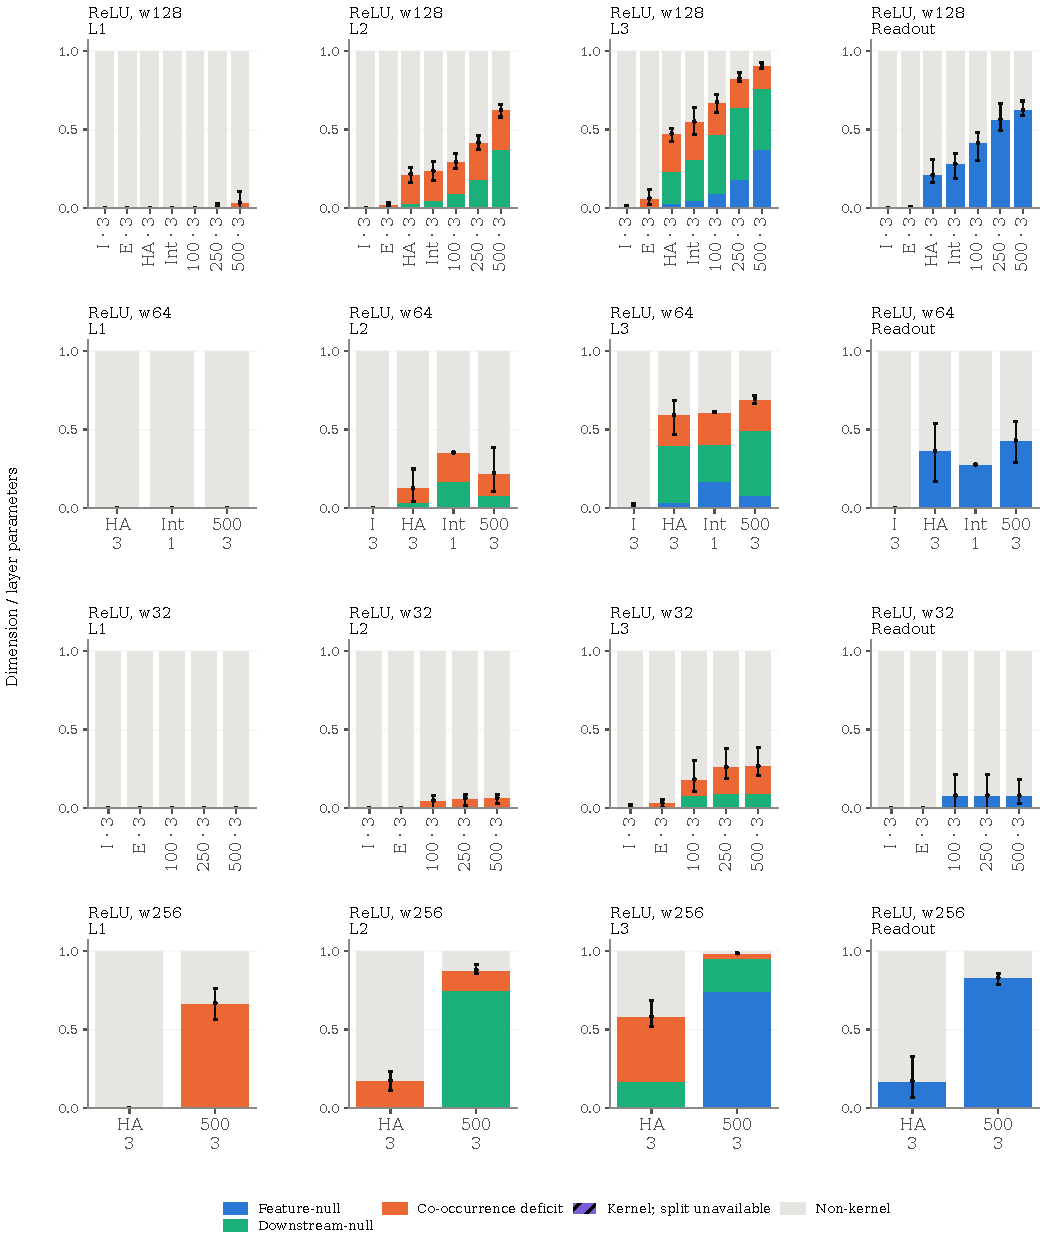
\includegraphics[width=6.272in]{compact_atomic_00.pdf}
\caption{Atomic decomposition across the indicated models and layers. Models use MNIST unless labeled SVHN; w and d denote width and hidden depth. Panels show a layer across stages, or all editable layers at the stated endpoint. Heights are fractions of layer parameters; bars average seeds and whiskers span their kernel fractions. Seed counts follow each stage label, on a second line or after a dot. I, E, HA, Int and Val denote initialization, early fitting, high accuracy, interpolation and validation selection; numbers denote fixed epochs. Stages are grouped by milestone and then fixed epoch. For reduced-data models, $n$ is the retraining or analysis-set size as titled. Hatched kernels have no measured component split. Counts use the $10^{-9}$ rank rule; GELU late-stage counts and layers without a spectral gap remain threshold-dependent.}\label{fig:c-atomic-0}
\end{figure}
\begin{figure}[!htbp]\centering
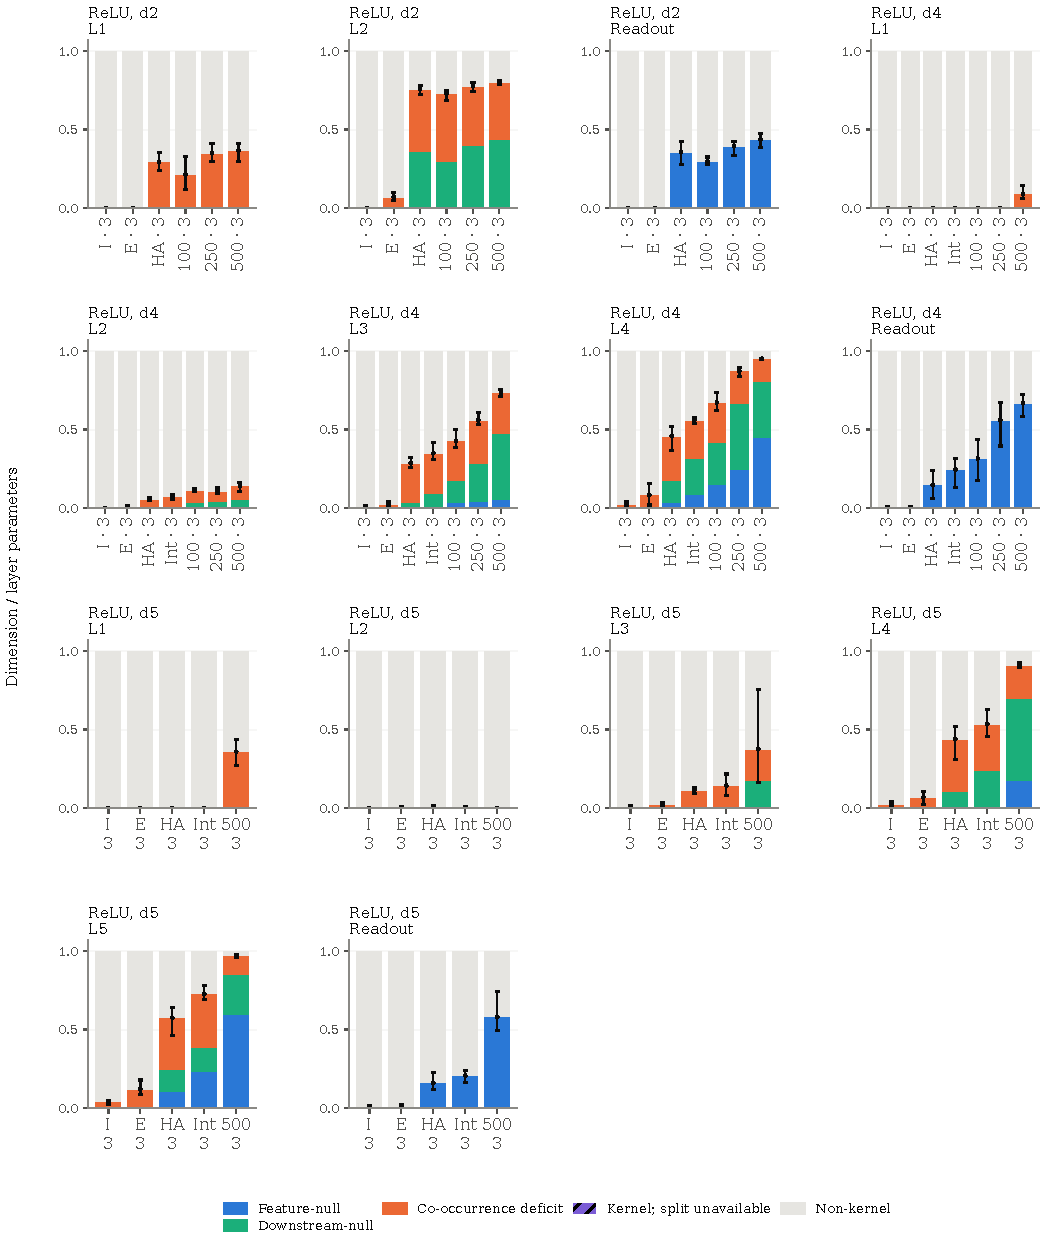
\includegraphics[width=6.272in]{compact_atomic_01.pdf}
\caption{Atomic decomposition across the indicated models and layers. Models use MNIST unless labeled SVHN; w and d denote width and hidden depth. Panels show a layer across stages, or all editable layers at the stated endpoint. Heights are fractions of layer parameters; bars average seeds and whiskers span their kernel fractions. Seed counts follow each stage label, on a second line or after a dot. I, E, HA, Int and Val denote initialization, early fitting, high accuracy, interpolation and validation selection; numbers denote fixed epochs. Stages are grouped by milestone and then fixed epoch. For reduced-data models, $n$ is the retraining or analysis-set size as titled. Hatched kernels have no measured component split. Counts use the $10^{-9}$ rank rule; GELU late-stage counts and layers without a spectral gap remain threshold-dependent.}\label{fig:c-atomic-1}
\end{figure}
\begin{figure}[!htbp]\centering
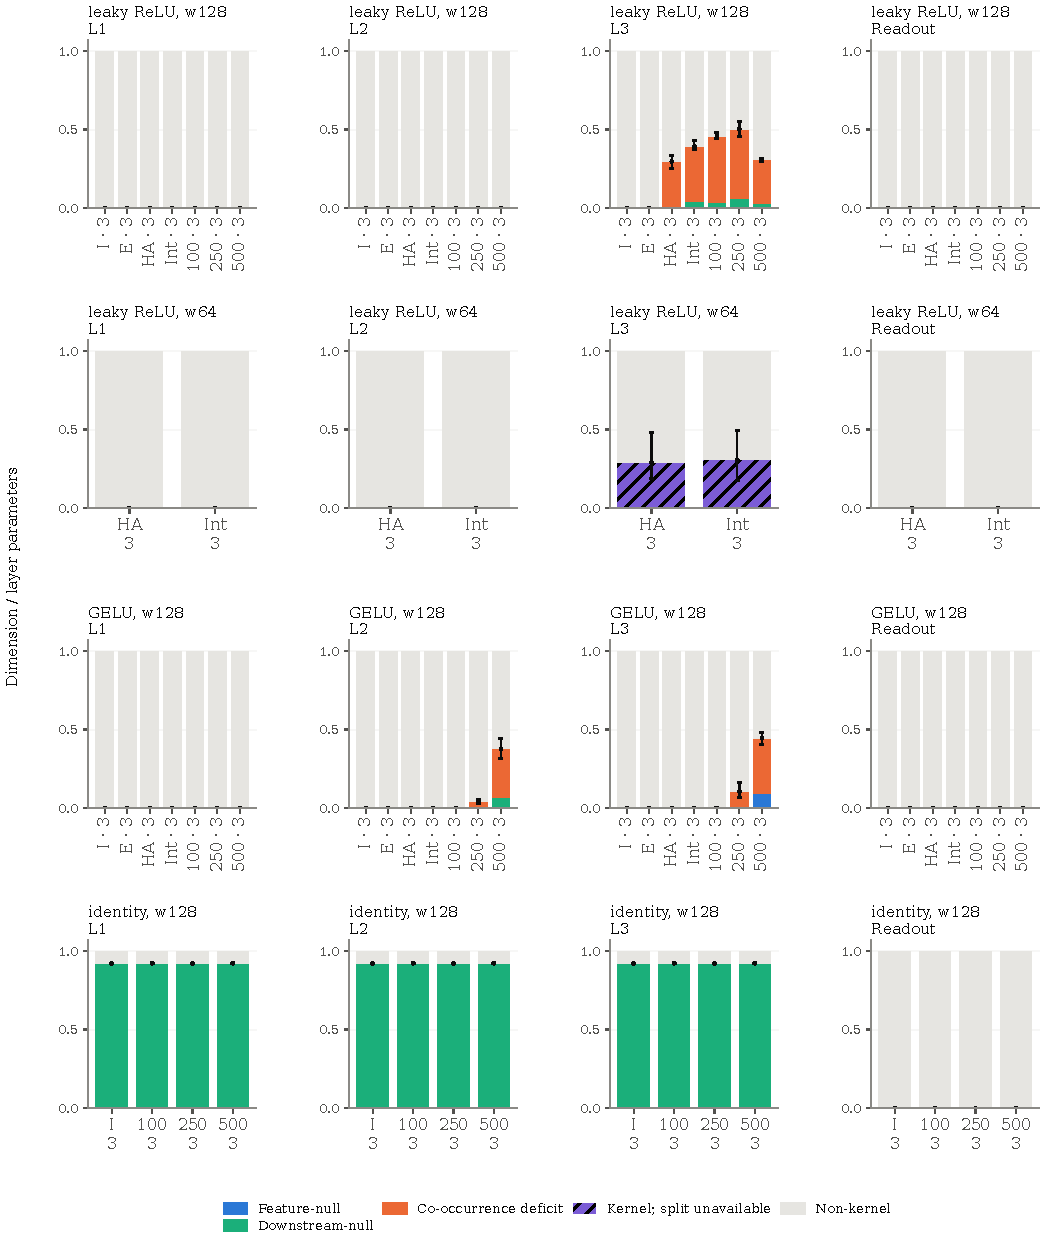
\includegraphics[width=6.272in]{compact_atomic_02.pdf}
\caption{Atomic decomposition across the indicated models and layers. Models use MNIST unless labeled SVHN; w and d denote width and hidden depth. Panels show a layer across stages, or all editable layers at the stated endpoint. Heights are fractions of layer parameters; bars average seeds and whiskers span their kernel fractions. Seed counts follow each stage label, on a second line or after a dot. I, E, HA, Int and Val denote initialization, early fitting, high accuracy, interpolation and validation selection; numbers denote fixed epochs. Stages are grouped by milestone and then fixed epoch. For reduced-data models, $n$ is the retraining or analysis-set size as titled. Hatched kernels have no measured component split. Counts use the $10^{-9}$ rank rule; GELU late-stage counts and layers without a spectral gap remain threshold-dependent.}\label{fig:c-atomic-2}
\end{figure}
\begin{figure}[!htbp]\centering
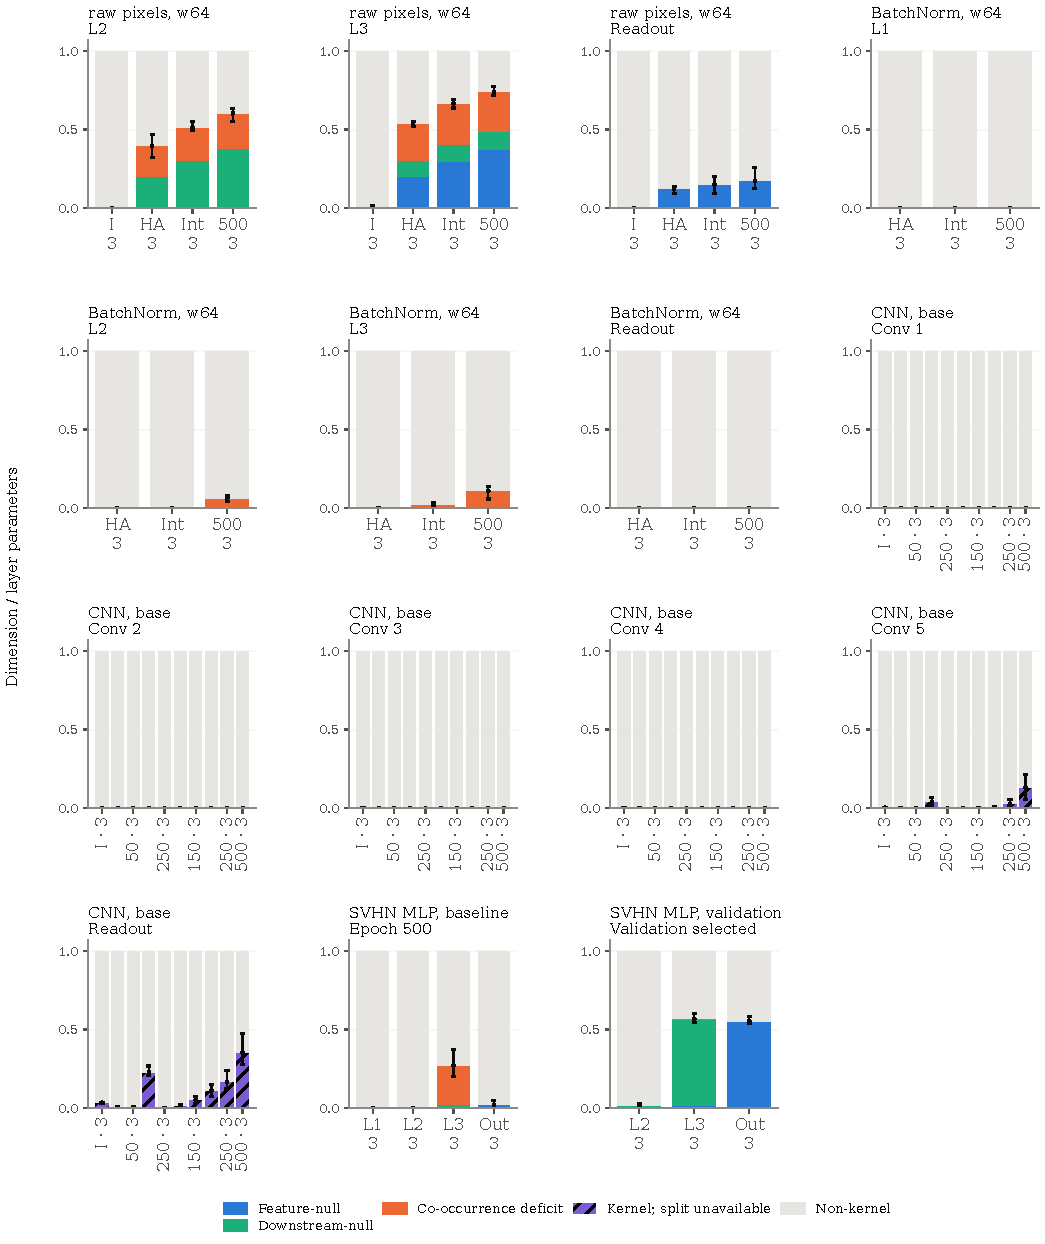
\includegraphics[width=6.272in]{compact_atomic_03.pdf}
\caption{Atomic decomposition across the indicated models and layers. Models use MNIST unless labeled SVHN; w and d denote width and hidden depth. Panels show a layer across stages, or all editable layers at the stated endpoint. Heights are fractions of layer parameters; bars average seeds and whiskers span their kernel fractions. Seed counts follow each stage label, on a second line or after a dot. I, E, HA, Int and Val denote initialization, early fitting, high accuracy, interpolation and validation selection; numbers denote fixed epochs. Stages are grouped by milestone and then fixed epoch. For reduced-data models, $n$ is the retraining or analysis-set size as titled. Hatched kernels have no measured component split. Counts use the $10^{-9}$ rank rule; GELU late-stage counts and layers without a spectral gap remain threshold-dependent.}\label{fig:c-atomic-3}
\end{figure}
\FloatBarrier




\paragraph{Activation, normalization and dataset comparisons.}\label{app:activations}\label{app:bn}\label{app:raw}\label{app:svhn}
The same measurements distinguish several ways of obtaining an invariant subspace. Leaky ReLU retains a late hidden-layer kernel through cancellations across units, despite having no exactly inactive negative piece. GELU develops broad approximate tails; its late numerical kernels have no clear spectral gap. BatchNorm leaves substantially smaller kernels, even at matched fitting stages, while the raw-pixel and SVHN comparisons show that representation and fitting conditions also affect their size. The preceding panels include these models, and the invariant subspace and transition comparisons below use the same protocols. Predictive-performance tables are retained in Appendix~\ref{app:performance}; training recipes are in Appendix~\ref{app:methods-activations} and Appendix~\ref{app:methods-data}.

\paragraph{Large layers and numerical resolution.}


For the width-512 MLP, randomized rank calculations resolve the third hidden-layer and readout ranks in two seeds. The second hidden layer has a rank lower bound. Table~\ref{tab:c-wide-ranks} reports each result in that form, so an unresolved rank remains distinct from a measured kernel dimension.
\begin{table}[!htbp]\centering
\caption{Width-512 ReLU MLP at epoch 500, 10,000 analysis images. A resolved numerical rank determines the corresponding nullity; a rank lower bound gives only a nullity upper bound.}\label{tab:c-wide-ranks}
\small\begin{tabular}{llrrr}\toprule
Layer & Seed & Parameters & Rank & Kernel dimension\\\midrule
L2 & 0 & 262656 & $\ge8192$ & $\le254464$\\
L3 & 0 & 262656 & $560$ & $262096$\\
Readout & 0 & 5130 & $360$ & $4770$\\
L2 & 1 & 262656 & $\ge8192$ & $\le254464$\\
L3 & 1 & 262656 & $659$ & $261997$\\
Readout & 1 & 5130 & $430$ & $4700$\\
\bottomrule\end{tabular}\end{table}
\FloatBarrier

The fine-tuned ViT has a different source of exact directions. LayerNorm identities give a compatible invariant subspace in the final MLP and readout, checked in all fine-tuned seeds. Table~\ref{tab:c-native-exact} separates these constructed spaces from counting lower bounds on tangent nullity. The full atomic ranks of the large ViT layers remain unresolved. The architecture is described in Appendix~\ref{app:methods-activations}, and the finite-radius results are in Appendix~\ref{app:native-vit}.
\begin{table}[!htbp]\centering
\caption{ViT-B/16 on RESISC45. Constructed exact dimensions are checked in three fine-tuned seeds. Counting lower bounds use 10,000 images and 45 outputs; they bound tangent nullity without constructing additional invariant subspaces.}\label{tab:c-native-exact}
\small\begin{tabular}{lrrrr}\toprule
Layer & Parameters & Exact space & Kernel lower bound & \shortstack{Remaining kernel\\lower bound}\\\midrule
First MLP affine layer & 2,362,368 & 3,072 & 1,912,368 & 1,909,296\\
Second MLP affine layer & 2,360,064 & 3,073 & 1,910,064 & 1,906,991\\
Readout & 34,605 & 45 & --- & ---\\
\bottomrule\end{tabular}\par\smallskip\footnotesize The remaining-kernel bound subtracts the constructed exact dimension from the full-kernel counting bound.
\end{table}

\paragraph{Approximate atomic directions.}
A numerical kernel counts directions below the tight rank threshold. Larger singular-value thresholds also include directions with a small, nonzero first-order output response. The next panels compare these two counts across the measured training trajectories, using the same relative thresholds across models and keeping every measured layer. The approximate spaces can occupy a substantial fraction of a layer even when its tight-threshold kernel is small. For GELU, a late-stage count without a spectral gap is a threshold-dependent numerical quantity.

\begin{figure}[!htbp]\centering
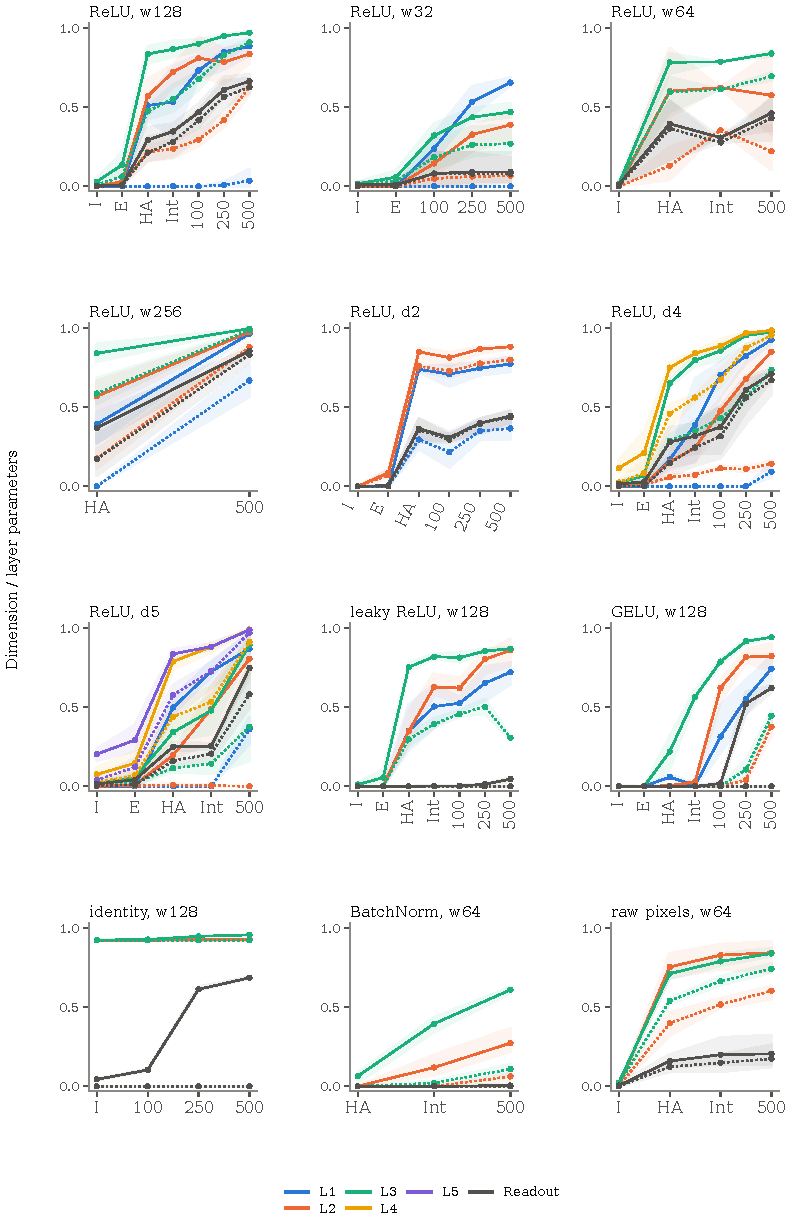
\includegraphics[width=4.754in]{compact_tails_part1.pdf}
\caption{Approximate atomic dimensions for models measured at multiple training stages, with all measured layers shown. MNIST is used unless labeled SVHN; layer numbers refer to hidden layers or convolutional layers. Solid curves count singular values at most $10^{-3}\sigma_1$ and dotted curves use $10^{-9}\sigma_1$, each divided by layer parameter count. Lines are seed means and bands are seed ranges. Missing measurements remain gaps. Stage positions are categorical, with abbreviations as in the atomic panels.}
\label{fig:atomic-tails}
\end{figure}
\begin{figure}[!htbp]\centering
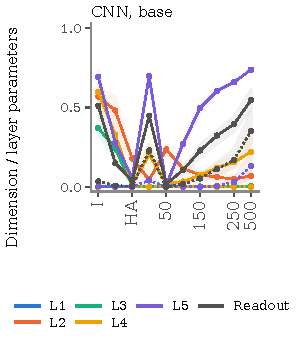
\includegraphics[width=1.804in]{compact_tails_part2.pdf}
\caption{Continued. Approximate atomic dimensions for models measured at multiple training stages, with all measured layers shown. MNIST is used unless labeled SVHN; layer numbers refer to hidden layers or convolutional layers. Solid curves count singular values at most $10^{-3}\sigma_1$ and dotted curves use $10^{-9}\sigma_1$, each divided by layer parameter count. Lines are seed means and bands are seed ranges. Missing measurements remain gaps. Stage positions are categorical, with abbreviations as in the atomic panels.}

\end{figure}
\FloatBarrier


\paragraph{Selective units and channels within the atomic kernel.}
For a ReLU unit, an incoming edit that annihilates the features of all samples on which it is active preserves its frozen activation on every sample. This gives an explicit part of the atomic kernel. With $\mathcal A_j$ the active sample set of unit $j$ and $\mathcal H_{\ell j}^{\rm act}(X)$ its augmented active-feature span, its dimension is
\[
 \dim G_\ell^{\rm sel}(X)
 =\sum_j\left(n_{\ell-1}+1-\dim\mathcal H_{\ell j}^{\rm act}(X)\right).
\]
An active set with too few samples leaves free directions by sample count alone. Further directions arise when its features span less than their count permits. The CNN construction imposes the analogous condition on all active patches of a channel.

The selective-space panels include the full MLP width and depth sweeps on both the 10,000-image analysis set and all 60,000 training images, together with the base MNIST and SVHN CNN trajectories. The CNN width endpoints are reported in Appendix~\ref{app:cnn-width}. Selective spaces often account for most of the hidden atomic kernel in fitted ReLU models. The unit-decomposition panels separate directions confined to one unit from the remaining directions that require cancellation across different units. These distinctions matter for leaky ReLU: class selectivity alone does not explain its atomic kernel, because negative-side slopes remain nonzero.


\begin{figure}[!htbp]\centering
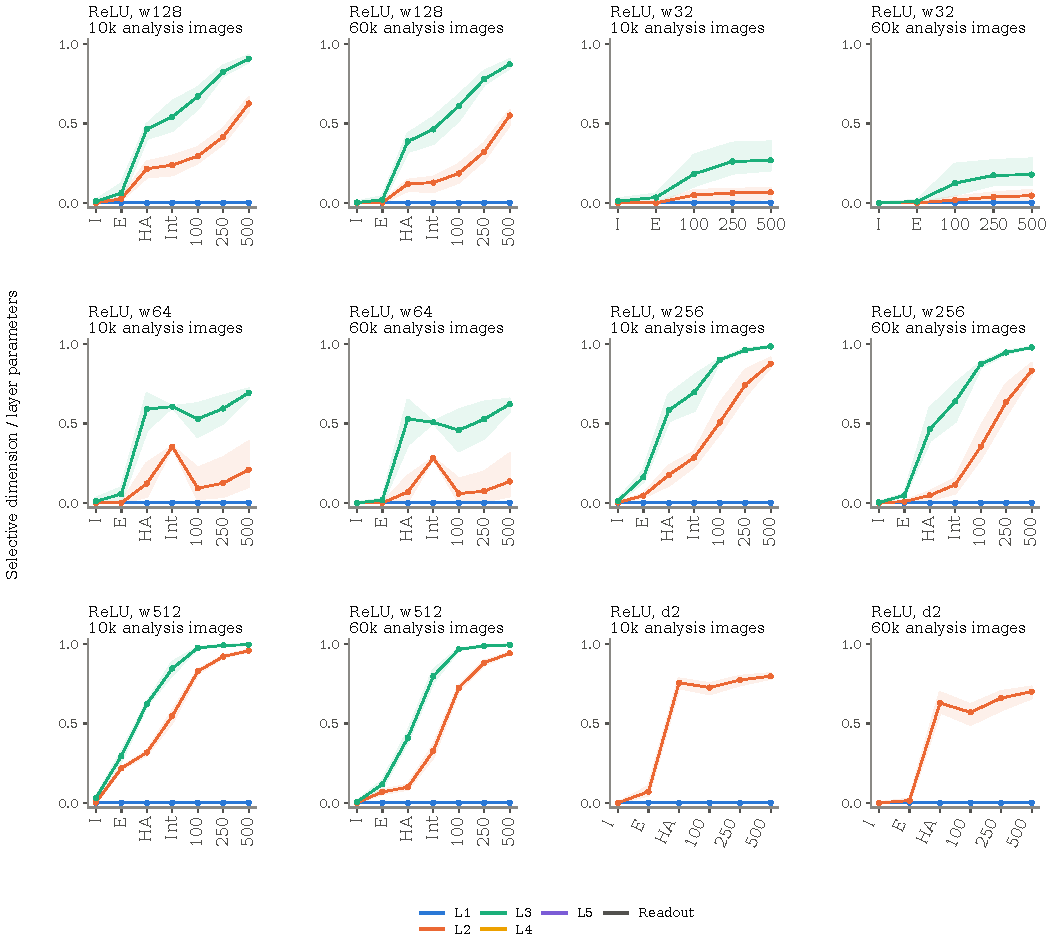
\includegraphics[width=6.315in]{compact_selective_part1.pdf}
\caption{Selective dimension as a fraction of layer parameters, across all tested stages and analysis-set sizes. MNIST is used unless labeled SVHN. Colors identify hidden layers or convolutional layers; lines are seed means and bands span seeds. MLP spaces constrain each unit on its active samples; CNN spaces constrain each channel on its active input patches. A zero identifies an empty selective construction; the full atomic kernel can still contain other directions. Stage abbreviations follow the atomic panels.}
\end{figure}
\begin{figure}[!htbp]\centering
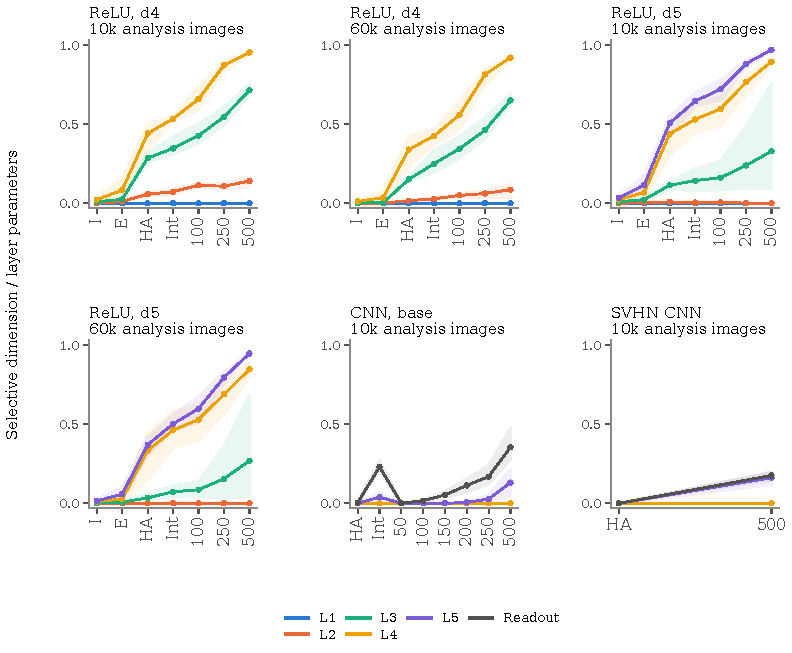
\includegraphics[width=4.754in]{compact_selective_part2.pdf}
\caption{Continued. Selective dimension as a fraction of layer parameters, across all tested stages and analysis-set sizes. MNIST is used unless labeled SVHN. Colors identify hidden layers or convolutional layers; lines are seed means and bands span seeds. MLP spaces constrain each unit on its active samples; CNN spaces constrain each channel on its active input patches. A zero identifies an empty selective construction; the full atomic kernel can still contain other directions. Stage abbreviations follow the atomic panels.}
\end{figure}
\begin{figure}[!htbp]\centering
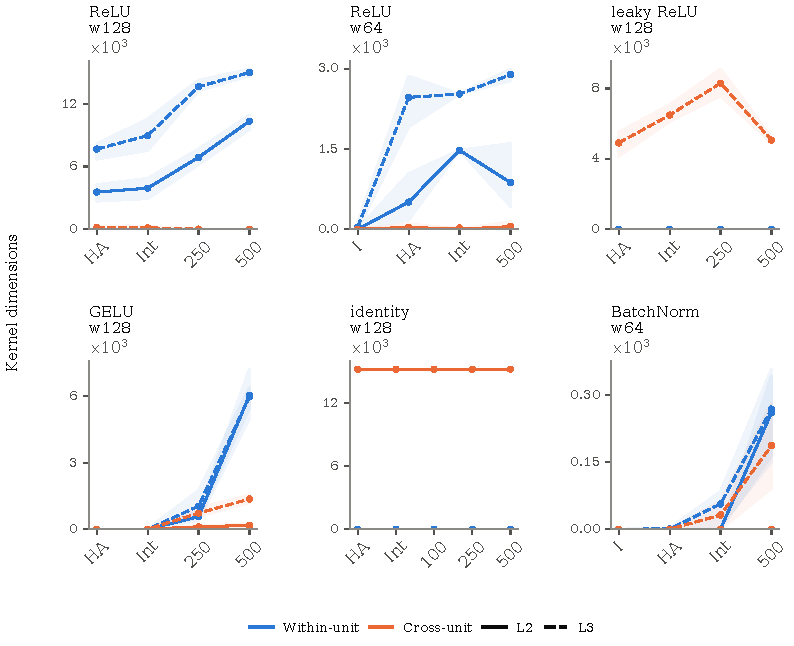
\includegraphics[width=4.762in]{compact_neuron.pdf}
\caption{Within-unit and cross-unit kernel dimensions for MNIST MLPs. Each panel combines L2 and L3, distinguished by line style. Curves are seed means and bands span seeds. ReLU within-unit directions agree with the selective construction where containment checks pass. Leaky-ReLU and GELU per-unit operators use their actual slopes; late GELU counts remain numerical threshold-dependent quantities.}
\end{figure}
\FloatBarrier


The channel-level CNN measurements provide a concrete view of selectivity. Figure~\ref{fig:cnn-units} shows which real inputs activate each late convolutional channel. The images reveal class-specific stroke patterns in this example; the preceding panels provide the corresponding dimensions across seeds and settings.


\begin{figure}[!htbp]\centering
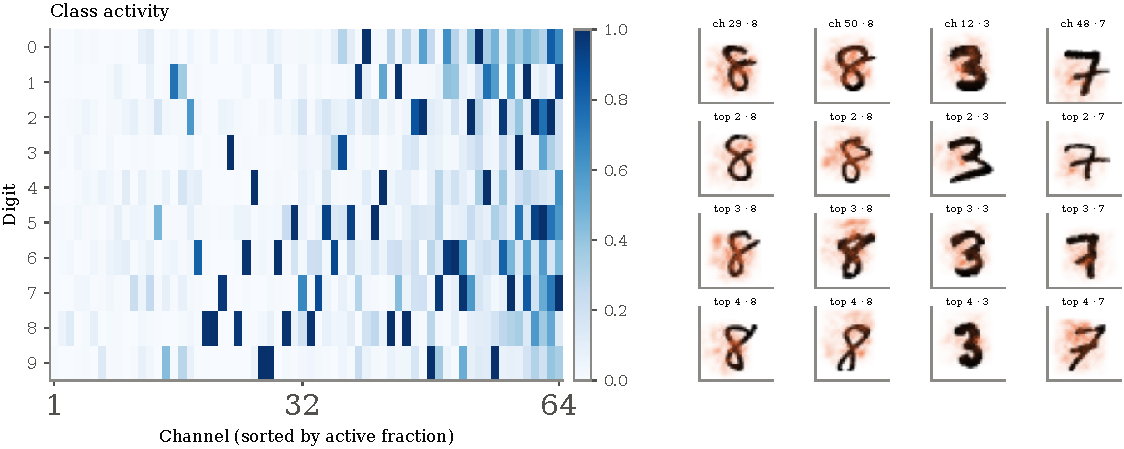
\includegraphics[width=.60\linewidth,height=.18\textheight,keepaspectratio]{cnn_units_wide.pdf}
\caption{Base MNIST CNN, conv5, seed 0 at epoch 500: class selectivity and the four most activating real images per channel, with input-gradient attribution. This qualitative example complements the multi-seed selective-space measurements.}\label{fig:cnn-units}
\end{figure}\FloatBarrier

\subsubsection{Finite-radius tests of atomic spaces}
\label{app:rays}\label{app:radius-full}
A Jacobian kernel describes the first-order response. We test the actual network along its directions to establish how far the frozen invariance persists. Following Appendix~\ref{app:methods-radius}, we compare single-layer kernels, approximate singular tails, generic directions, and edits to dead-unit incoming or outgoing coordinates. We record both the first gate crossing and the first output change exceeding $10^{-3}$.

For the width-128 ReLU MLP, the readout kernel and outgoing weights of zero features stay flat throughout the scan. Incoming edits to dead units remain flat until the units reactivate. Hidden-layer directions often cross gates before their output response becomes visible. Figure~\ref{fig:rays-overview} separates these mechanisms, including the dead-unit controls, with only one layer edited at a time. The multilayer invariant subspace scans in Appendix~\ref{app:composition-results} test simultaneous edits to several layers.


\begin{figure}[!htbp]\centering
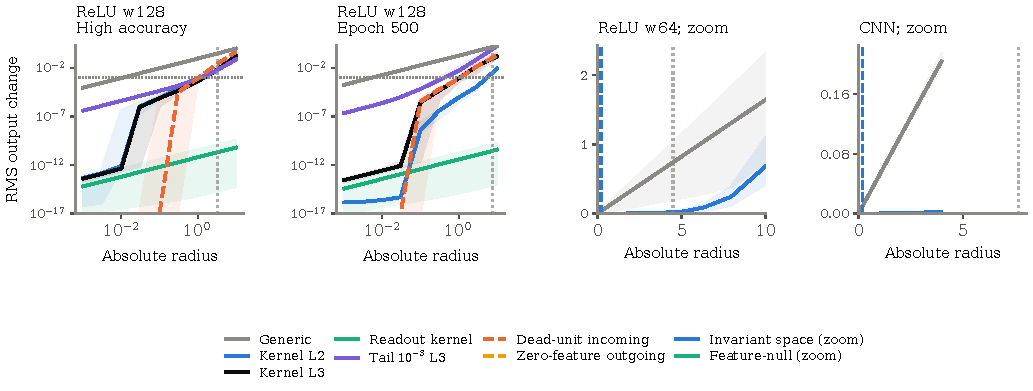
\includegraphics[width=6.195in]{atomic_rays_zoom.pdf}
\caption{Atomic rays and zoomed invariant subspace responses on MNIST. Left pair: width-128 ReLU single-layer kernels, approximate tails and dead-unit controls, with medians of 32 probes per seed and ranges across three seeds; the generic reference edits the whole network. Right pair: seed-0 width-64 MLP and CNN slices, with medians and 10th--90th percentiles over angles; feature-null curves use their own slice axis. These panels use linear axes to resolve visible drift after a first crossing (blue dashed marker). Gray vertical dotted markers give $0.1\|\theta\|_2$; the left panels also mark output visibility at $10^{-3}$. Blue and green retain the invariant-direction and feature-null roles across panels, while the legend distinguishes atomic kernels from multilayer invariant subspaces.}\label{fig:rays-overview}\label{fig:zoom-rays}
\end{figure}
\FloatBarrier


\paragraph{Activation controls.}
Leaky ReLU removes ReLU's exactly zero negative-side slope, while GELU replaces the kink by a smooth transition. Figure~\ref{fig:c-activation-rays} tests how these changes affect single-layer invariance in the width-128 MNIST models. It contrasts numerical kernel directions in L2 and L3 with a L3 approximate tail. Solid curves show the actual response and dashed curves the frozen response; lighter curves denote high accuracy and darker curves epoch 500. The generic curves perturb all layers and serve as a full-network sensitivity reference, so their amplitudes are not a matched single-layer comparison. 


\begin{figure}[!htbp]\centering
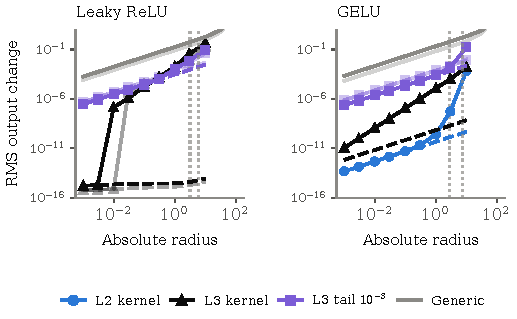
\includegraphics[width=3.105in]{activation_rays_square.pdf}
\caption{Leaky-ReLU and GELU width-128 MNIST MLPs, seed 0, at high accuracy and epoch 500. Single-layer kernel and approximate-tail directions separate frozen invariance from finite-distance output drift. The gray generic reference edits the full network. Gray vertical dotted lines mark $0.1\|\theta\|_2$ at each checkpoint.}\label{fig:c-activation-rays}
\end{figure}

\paragraph{Smooth activations and approximate atomic spaces.}
\label{app:gelu-eps}

For a smooth activation such as GELU, an exact atomic kernel can be empty. Approximate Jacobian kernels instead collect directions with a small first-order response; finite steps can still accumulate drift through activation curvature. Figure~\ref{fig:gelu-extended-rays} tests the L3 approximate kernel at the common sensitivity cutoff $10^{-3}$. All 256 sampled directions per seed and stage stay below output drift $10^{-3}$ through radius 1, while all exceed it by radius 10. The smaller response than generic L3 edits therefore has a finite measured extent.

\begin{figure}[!htbp]\centering
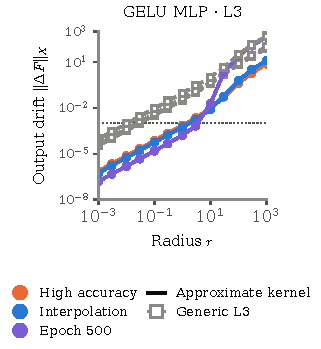
\includegraphics[width=1.924in]{gelu_rays_standard.pdf}
\caption{Extended GELU L3 rays in width-128 MNIST MLPs. The approximate kernel uses $\sigma(J_3)/\sqrt{s}\le10^{-3}$; generic controls edit the same layer. Lines show the mean and shading one sample SD of the within-seed medians over 256 rays, across three seeds. Colors identify the ReLU-matched training stages. The dotted line marks output drift $10^{-3}$.}\label{fig:gelu-extended-rays}
\end{figure}

The diagnostic $\widehat B(w)$ in Figure~\ref{fig:gelu-eps} is defined in Appendix~\ref{app:methods-radius}; it uses measured RMS preactivation displacements and base-point gains in place of uniform quantities. It exceeds measured transition by two to three orders of magnitude; local curvature is much smaller than its global bound along these probes.


\begin{figure}[!htbp]
\centering
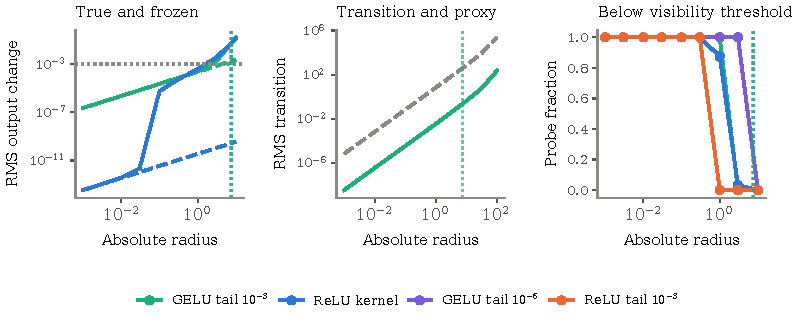
\includegraphics[width=4.786in]{gelu_rays_norm.pdf}
\caption{GELU approximate flatness and the diagnostic $\widehat B(w)$ from Appendix~\ref{app:methods-radius}. Seed-0 width-128 MNIST models at epoch 500. The left panel compares true (solid) and frozen (dashed) responses; the middle compares the transition norm with the diagnostic proxy (gray dashed); the right gives the fraction of probes below output change $10^{-3}$. Vertical dotted lines mark $0.1\|\theta\|_2$ in each model color. The proxy uses RMS displacements and base-point gains. Numerical late-stage kernels do not certify an exact analytic ocean.}
\label{fig:gelu-eps}
\end{figure}\begin{figure}[!htbp]
\centering
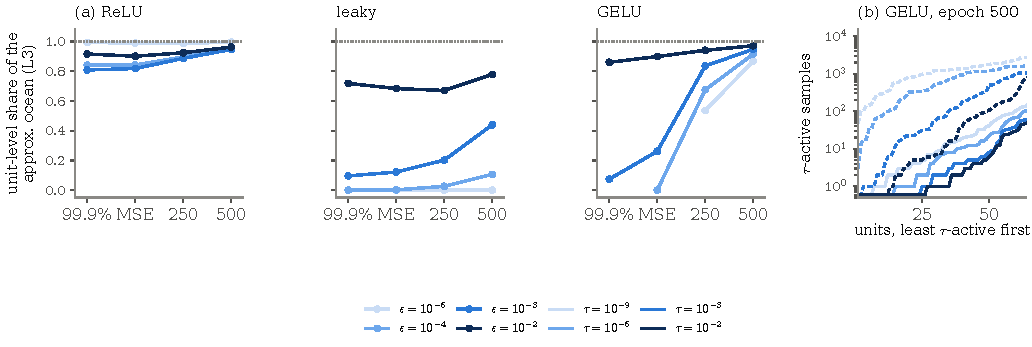
\includegraphics[width=6.194in]{soft_selectivity.pdf}
\caption{Soft selectivity under GELU: weak derivatives and concentrated active-input geometry accompany large approximate tails.}
\label{fig:gelu-soft}
\end{figure}


\FloatBarrier

\subsection{Multilayer invariant subspace construction and validation}
\label{app:composition-results}\label{app:cnn-branch}\label{app:selective}
Single-layer invariance leaves a further question: can several layers be edited at once while preserving the frozen outputs? An early-layer edit changes the inputs received by later layers, so individually invariant edits can interact. The received-space construction checks this compatibility. The construction plots follow the resulting dimensions over training for each attempted layer order and explicit subspace construction. Each curve is one seed. We show models measured at more than one epoch. Crosses mark zero retained dimension, including failed validations; unattempted constructions have no point.

For the tested width-64 full-data MNIST models, the layer orders recover the full atomic sum. CNN invariant subspaces retain almost that sum after removing directions at the numerical rank boundary. The reduced-data experiments in Appendix~\ref{app:training-data} show why compatibility must still be checked: different orders can give different invariant subspace dimensions from the same atomic spaces. We also report the raw-pixel, BatchNorm and SVHN comparisons. Full multilayer constructions have not been computed for every model in the MLP size sweeps, so their atomic dimensions alone do not establish equally large multilayer invariant subspaces.


\begin{figure}[!htbp]\centering
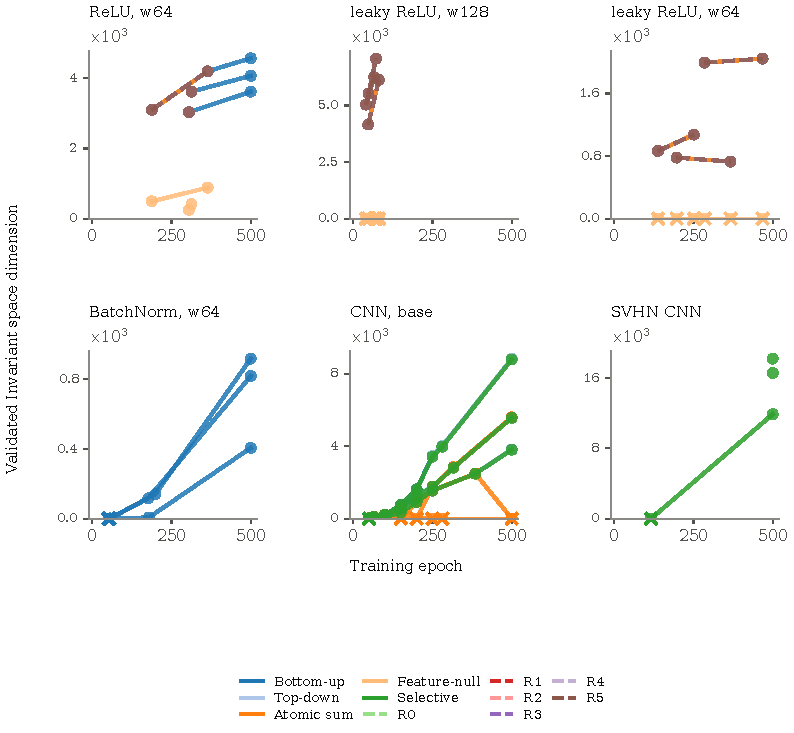
\includegraphics[width=4.762in]{construction_time_general_00.pdf}
\caption{Multilayer invariant subspace dimensions versus actual checkpoint epoch. Each curve is one seed; colors identify constructions, and dashed curves denote random layer orders R0--R5. Coincident curves have equal retained dimensions. Crosses mark zero retained dimension, including failed validations; unattempted constructions have no point. MNIST is used unless labeled SVHN. Only models with a trajectory measured within at least one seed are shown.}
\end{figure}
\FloatBarrier


\subsection{Radius tests}
\label{app:radius-results}
\subsubsection{Directional certificates}
\label{app:radius-certificates}
The invariant spaces permit substantially larger certified grid radii than generic directions across the tested architectures (Figure~\ref{fig:radius-certificates-all}). The early CNN spaces remain safe throughout the scan but contain few directions; later spaces are much larger and have shorter measured radii. Exact ViT feature-null and LayerNorm-shift families remain at numerical precision throughout their extended scans.

\begin{figure}[!htbp]\centering
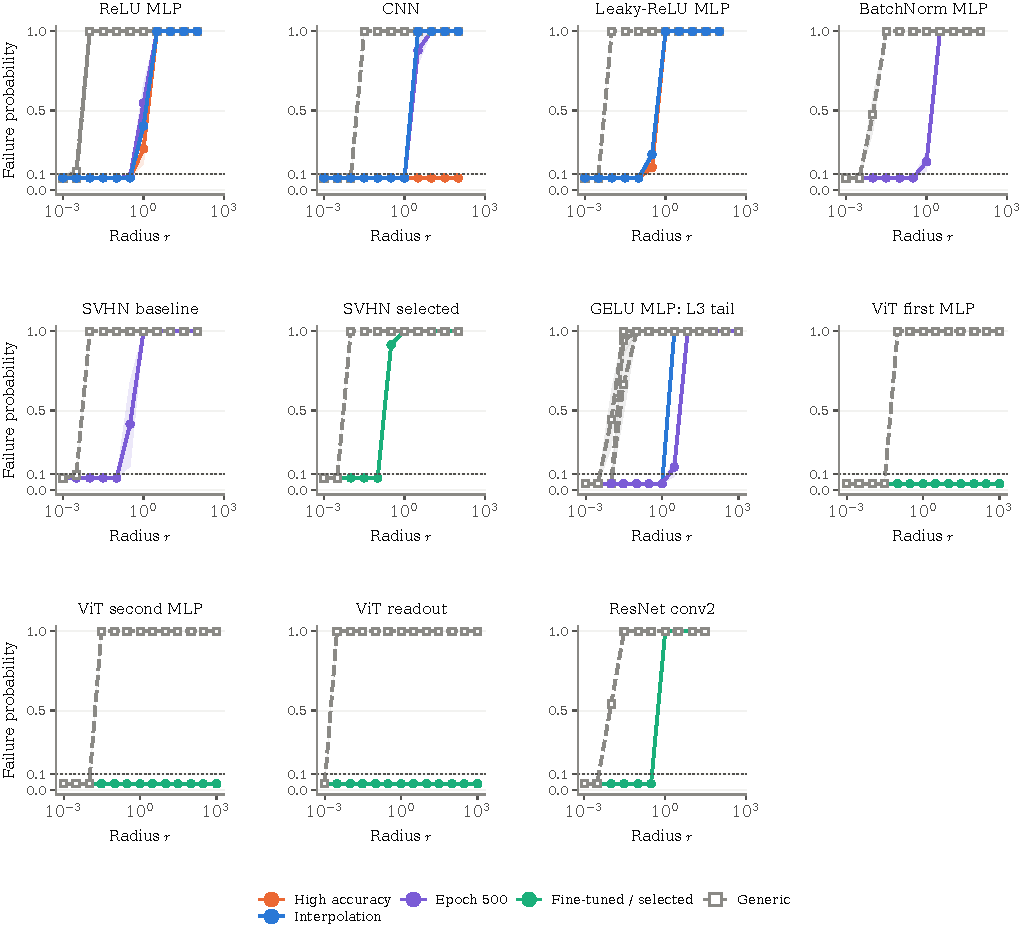
\includegraphics[width=6.149in]{radius_certificates.pdf}
\caption{Failure-probability upper bounds at absolute output tolerance $10^{-3}$. Solid curves: constructed spaces; dashed curves: generic controls. Colors denote training stages; shading is one sample SD across available seeds. The dotted line marks $10\%$ allowed failures. Bounds hold with $95\%$ simultaneous confidence over all 1126 comparisons in this figure; lines connect tested radii. GELU uses the approximate L3 kernel with $\sigma(J_3)/\sqrt{s}\le10^{-3}$. ViT shows first-MLP and readout feature-null edits and second-MLP downstream-null edits; ResNet shows the final convolution's selective family.}
\label{fig:radius-certificates-all}\label{fig:radius-variants}
\end{figure}

\FloatBarrier

\subsubsection{Ray responses}\label{app:radius-responses}
The actual and frozen responses show where activation changes become visible along the same edits. The following comparisons include wider networks, different activations and input representations. Their descriptive bands summarize seed variation; the certificates above use independent-ray failure counts.
\begin{figure}[!htbp]\centering
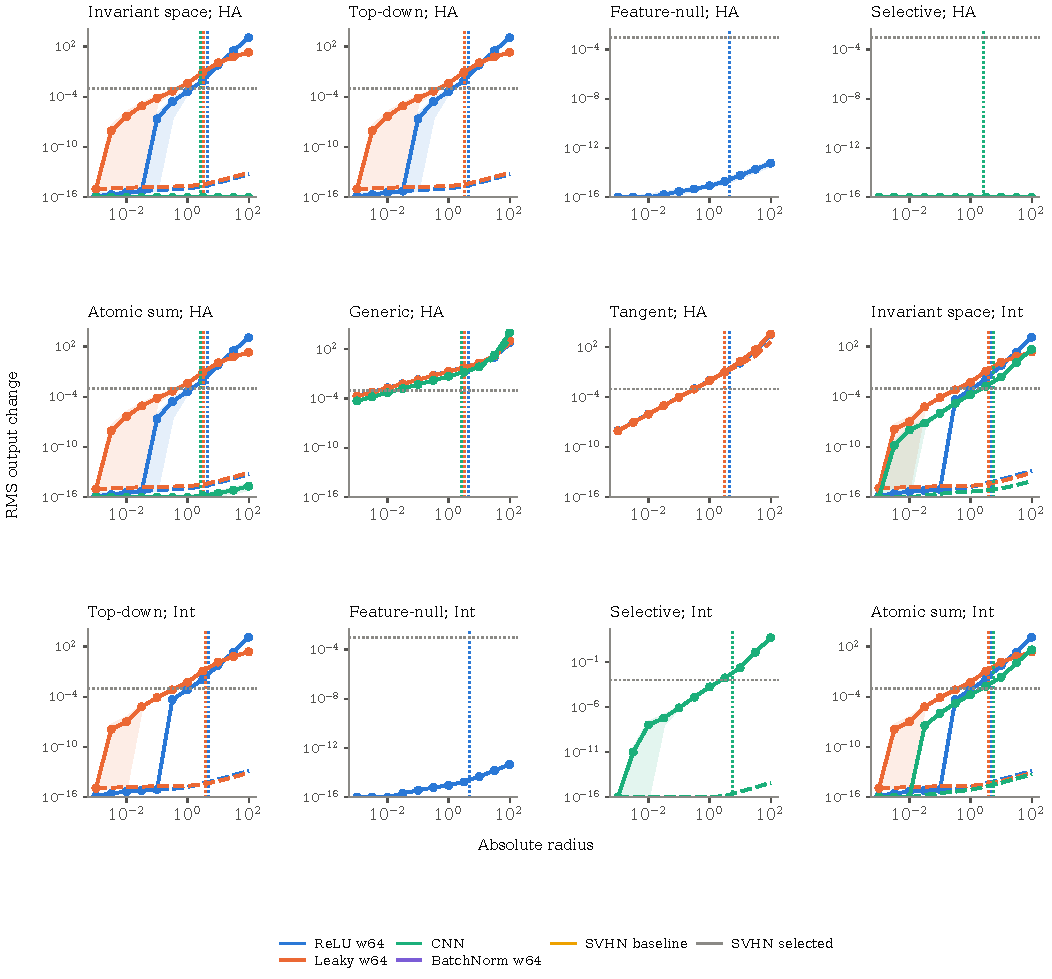
\includegraphics[width=6.313in]{rays_joint_0.pdf}
\caption{Absolute-radius responses across architectures and activations. Each panel fixes the training stage and direction family; only width 64 is shown for leaky ReLU. The Invariant subspace panels combine MLP bottom-up constructions with the CNN received-space construction; Selective panels retain the separate CNN selective candidates. Solid and dashed curves give actual and frozen responses, averaged over seed medians, with seed ranges shaded. Dotted vertical lines mark one tenth of the network norm; the horizontal dotted line marks output change $10^{-3}$. Missing curves indicate unmeasured model--stage combinations.}\label{fig:appendix-ray-comparison}
\end{figure}
\begin{figure}[!htbp]\centering
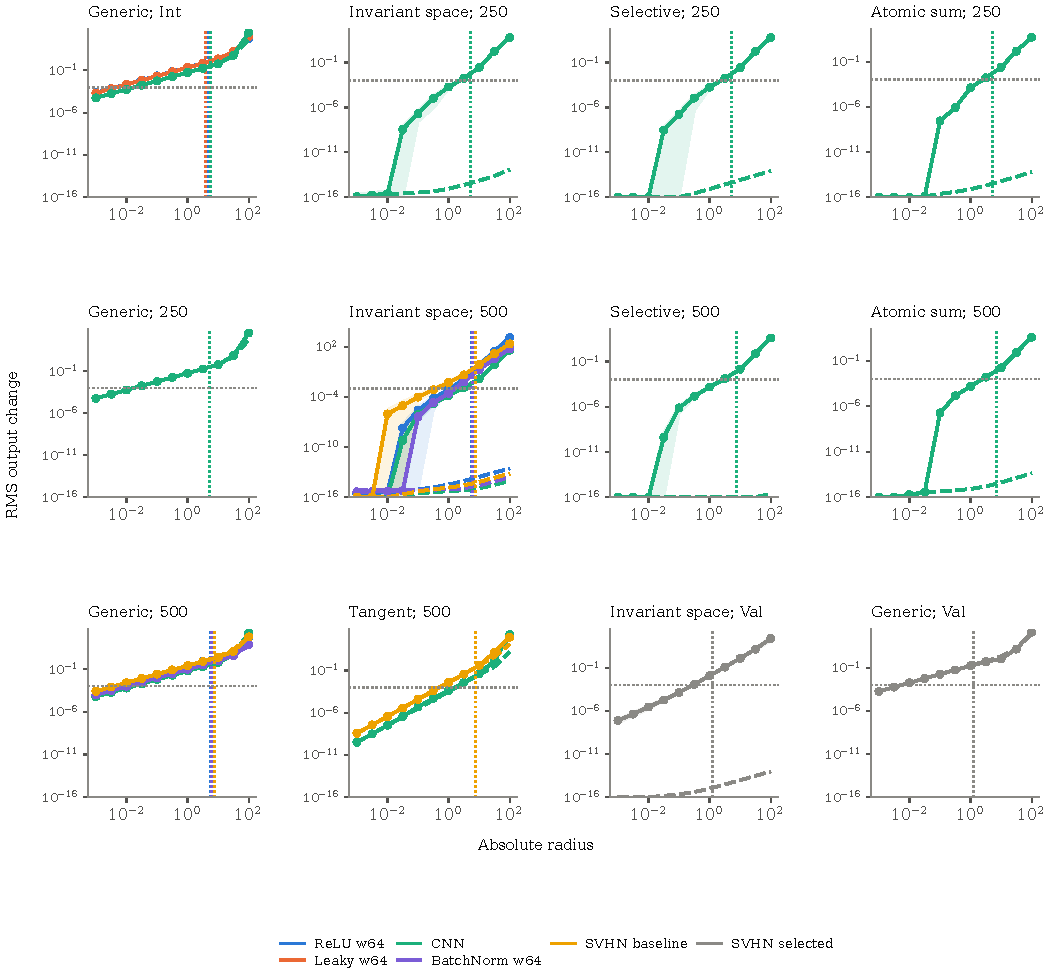
\includegraphics[width=6.313in]{rays_joint_1.pdf}
\caption{Additional stages and direction families, with the conventions of Figure~\ref{fig:appendix-ray-comparison}.}
\end{figure}
\FloatBarrier


\subsection{Activation-transition potential}
\label{app:transition}
We next ask how departures from the base activation pattern contribute to the output response. The local residual $\rho_\ell(w)$ measures departure from the base affine activation at layer $\ell$, and the edited frozen tail $T_\ell(w)$ propagates it through the remaining layers. Their vector contributions add to the activation-transition term,
\[
 A_X^{\rm tr}(w)=\sum_\ell T_\ell(w)\rho_\ell(w).
\]
We measure its magnitude relative to the actual output change, $\|A_X^{\rm tr}(w)\|_X/\|\Delta F_X(w)\|_X$, using 256 paired directions per checkpoint and radius. This ratio can exceed one when the transition and frozen responses partly cancel.

The panels compare width-128 ReLU, leaky-ReLU and GELU MLPs, the base CNN, and width-64 plain and BatchNorm MLPs. Single-layer perturbations identify where the response originates; full-network perturbations also include interactions between edited layers. The figures use absolute radii. The vertical dotted markers identify edits with Euclidean norm equal to 10\% of the network's parameter norm. An absolute radius is the norm of the full edit, including when only one layer moves. Each stage has its own marker color, and positions summarize the three seeds.
\begin{figure}[!htbp]\centering
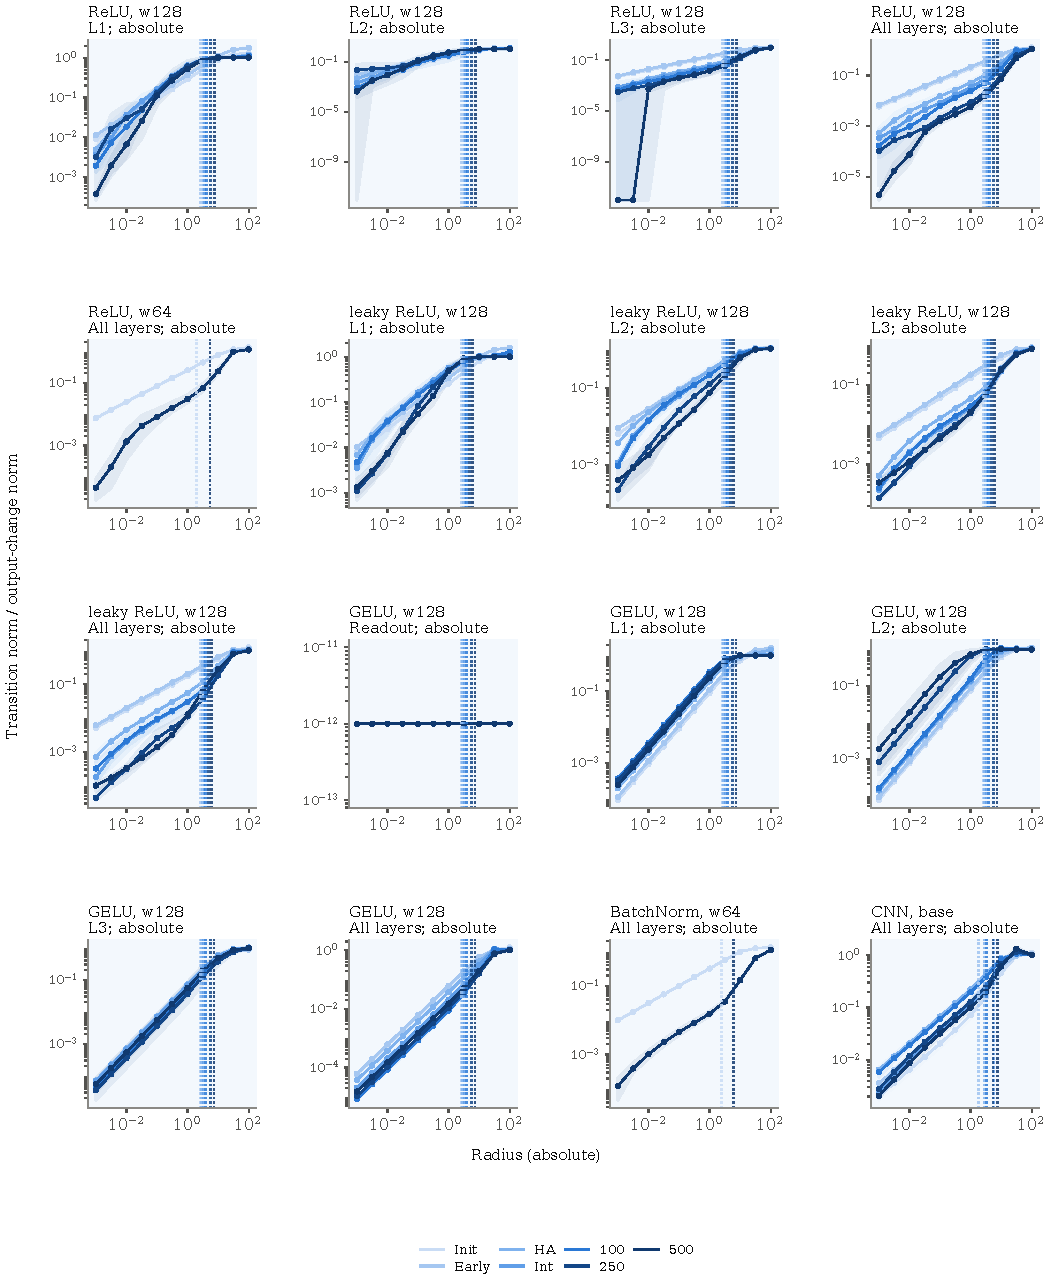
\includegraphics[width=6.313in]{absolute_transition_00.pdf}
\caption{Activation-transition share $\|A_X^{\rm tr}\|_X/\|\Delta F_X\|_X$ for the indicated editable layers. Curves show means of within-seed medians over 256 directions; bands span seeds. Dotted vertical lines mark edits of norm $0.1\|\theta\|_2$. Ratios above one indicate cancellation with the frozen response. Values below $10^{-12}$ use that plotting floor.}
\end{figure}
\FloatBarrier


\paragraph{Response magnitudes and cancellation across layers.}
A large ratio of transition norm to output-change norm can reflect a large activation residual or a small net output change caused by cancellation. Figure~\ref{fig:c-transition-details} distinguishes these cases. Its upper row compares the true, frozen and transition norms at one fixed absolute radius. Its lower row separates the propagated layer residuals and compares their summed norms with the norm of their vector sum. The gap between those two quantities measures cancellation across layers.
\begin{figure}[!htbp]\centering
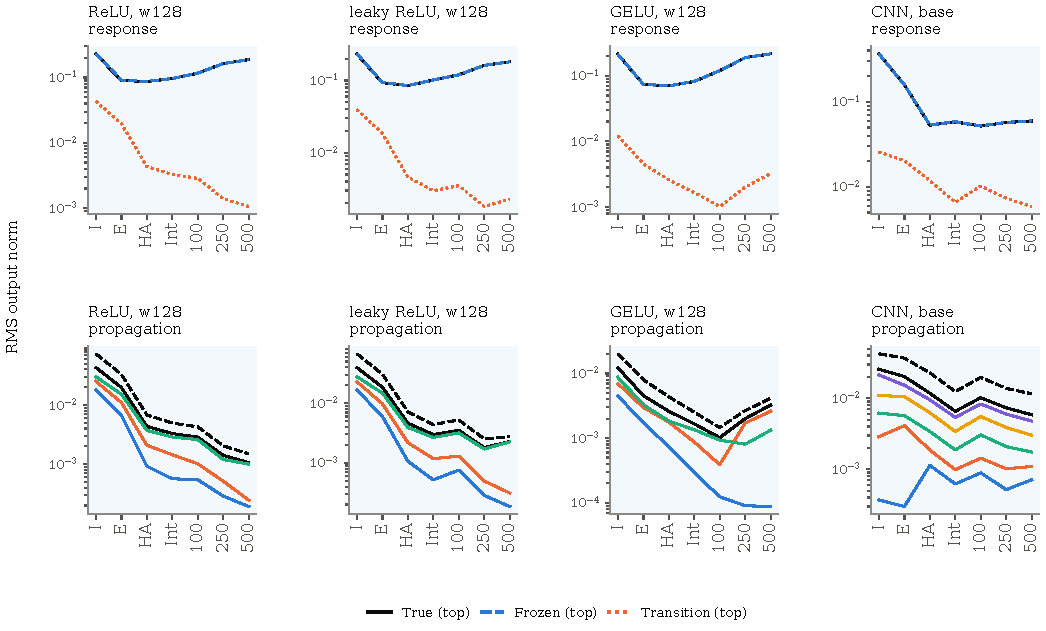
\includegraphics[width=6.274in]{absolute_transition_details.pdf}
\caption{Response magnitudes and layerwise propagation on 256 full-network directions per seed at absolute radius 1. Upper panels separate true, frozen and transition norms. Lower panels show each propagated layer residual in the atomic-plot layer colors, their sum of norms (black dashed), and the norm after vector summation (black solid). Their separation measures cancellation across layers. Curves average within-seed medians over three seeds. Values below $10^{-16}$ use that plotting floor.}\label{fig:c-transition-details}
\end{figure}
\FloatBarrier


\paragraph{Margins and activation curvature.}
The margin distributions show how far preactivations lie from the activation's transition region. ReLU and leaky ReLU are affine on each side of zero; GELU approaches affine behavior in both tails. Sigmoid, tanh and softplus provide further smooth-tail examples in Appendix~\ref{app:radius-proof}. For a fixed preactivation displacement, remaining far enough into an affine or low-curvature region makes the activation residual zero or small. This requires the entire displacement to remain in that region: a large initial margin alone does not protect an edit that returns to the transition region. Downstream propagation then determines how much of the local residual reaches the output.
\begin{figure}[!htbp]\centering
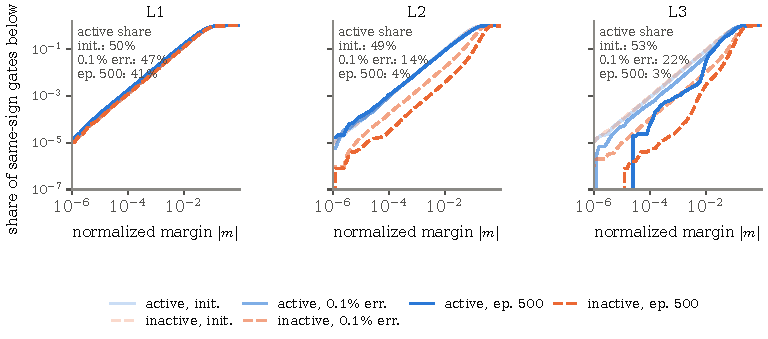
\includegraphics[width=4.606in]{paper_margins_mnist.pdf}
\caption{Sign-conditional distributions of normalized preactivation margins in the MNIST activation comparison. Solid and dashed lines condition on active and inactive gates; panels also report active fractions.}\label{fig:margins}
\end{figure}

\paragraph{CNN background and gate crossings.}
Digit images contain large background regions. A nearly zero preactivation at a background position can change sign while producing only a small activation residual. Counting these crossings therefore need not predict a large output response. Figure~\ref{fig:c-cnn-background} relates the number of conv1 crossings to their propagated contribution, separately for interior background, padding boundaries and digit patches. Each path follows training stages. The large background crossing counts at high accuracy have a small propagated contribution; later checkpoints suppress these crossings. This comparison measures the output importance of crossings rather than treating every changed gate as equally influential.

\begin{figure}[!htbp]\centering
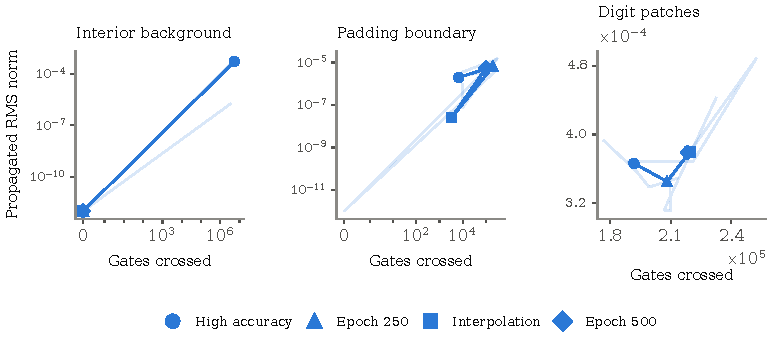
\includegraphics[width=4.629in]{background_trajectory.pdf}
\caption{Conv1 gate crossings and propagated residuals in the base MNIST CNN at layer-relative radius $0.01$. Each point is a training stage: within-seed medians over 128 matched directions, then means over three seeds; faint paths show individual seeds. Paths follow training order. Background and boundary panels use a horizontal scale linear up to one crossing and logarithmic above it; the digit panel uses linear axes to resolve its narrower range. Zero propagated contributions are drawn at $10^{-12}$.}\label{fig:c-cnn-background}
\end{figure}
\FloatBarrier


\subsection{Controlled training: margin regularization}
\label{app:controlled}


\paragraph{Margin regularization.}
The training objective in Appendix~\ref{app:methods-margin} penalizes preactivations near zero, encouraging larger margins from ReLU's switching boundary. We compare two penalty strengths with the unregularized width-64 MNIST control, using three paired seeds and each model's certified invariant subspace at epoch 500.

The penalty empties the near-zero preactivation region and delays the first gate crossing. Output visibility changes much less: its median remains at the control's grid radius in five of the six penalized runs, and moves to the next grid point in the remaining run (Table~\ref{tab:margin-summary}). The radius curves below show the separation between these two events. The penalty also increases parameter norms and worsens fitting, as reported in Appendix~\ref{app:performance}; it therefore changes more than margins alone.
\begin{table}[!htbp]\centering
\caption{Margin arms, seed order 0/1/2. First-crossing radii are medians over probes on a half-decade grid.}\label{tab:margin-summary}
\begin{tabular}{lrrr}\toprule
Arm & first crossing & visible radius & certified dimension\\\midrule
Control & .316/.0316/.0316 &3.16/3.16/3.16&3619/4573/4072\\
$\lambda=.01$ &1/1/1&10/3.16/3.16&4483/4715/4272\\
$\lambda=.1$ &3.16/.316/3.16&3.16/3.16/3.16&4997/5532/5305\\\bottomrule
\end{tabular}\end{table}

\begin{figure}[!htbp]
\centering
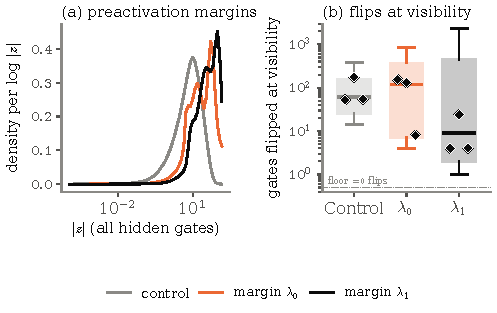
\includegraphics[width=2.979in]{margin_dists.pdf}
\caption{Margin penalties shift absolute preactivations away from zero. At first visible output change, penalized models have fewer gate crossings: early output-invisible flips have been removed.}
\label{fig:margin-dists}
\end{figure}


\paragraph{Invariant subspace response under the intervention.}
The next panels compare the control and both margin penalties under absolute edits. Each arm is tested in its own invariant subspace, with a dotted marker at one tenth of its network norm.

\begin{figure}[!htbp]\centering
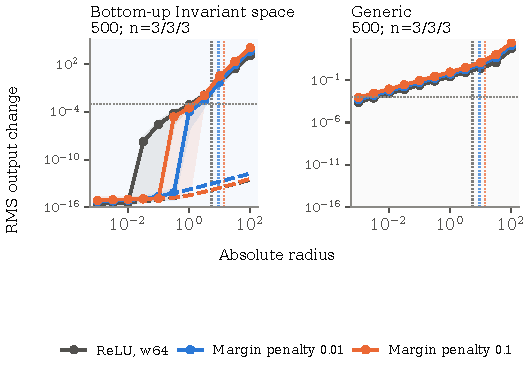
\includegraphics[width=3.191in]{rays_absolute_margin_00.pdf}
\caption{Margin-regularized and control networks at epoch 500. Solid/dashed curves show actual/frozen drift, with means and ranges over three seed medians. Dotted lines mark output drift $10^{-3}$ and edits of one tenth of each network's norm.}
\end{figure}
\FloatBarrier

\FloatBarrier

\section{Empirical results, extended version}
\label{app:empirical-results}\label{app:ablations}\label{app:persistence-results}
The empirical comparisons ask how ocean geometry changes with network scale, learned representations, data and continued training. Activation, normalization and dataset ablations are included alongside the corresponding measurements in Appendix~\ref{app:theoretical-support}. Their implementation is described in Appendix~\ref{app:experiments}.

\subsection{Fine-tuned ViT on RESISC45}


\label{app:vit}\label{app:native-vit}


The final ViT layers contain exact invariant families with the same feature- and downstream-based interpretation as in smaller networks. We follow the protocol in Appendix~\ref{app:methods-common-families}. Compatible combinations give 3,117 feature-null directions, or 6,190 directions when LayerNorm shifts are included; these constructions do not exhaust the unresolved full atomic kernels.

\subsubsection{Layerwise results}
\label{app:vit-common}
The common protocol recovers the same 6,190 exact directions in all three seeds (Table~\ref{tab:vit-common}). Feature-null edits account for the first MLP layer and readout; the second MLP layer contributes downstream-null LayerNorm shifts. No additional selective directions are found.

\begin{table}[!htbp]\centering
\caption{ViT family dimensions under the common protocol (Appendix~\ref{app:methods-common-families}). Slash-separated entries give seeds 0/1/2; selective and approximate dimensions exclude exact-family overlap.}
\label{tab:vit-common}
\small\setlength{\tabcolsep}{5pt}
\begin{tabular}{lrrr}\toprule
Family & First MLP layer & Second MLP layer & Readout\\\midrule
Feature-null & 3,072 & 0 & 45\\
Additional downstream-null & 0 & 3,073 & 0\\
Additional selective & 0 & 0 & 0\\\midrule
Feature tail & 0 & 3,068/1,534/2,301 & 0\\
Downstream tail & 768/768/0 & 0 & 0\\\bottomrule
\end{tabular}
\end{table}

All sampled exact-family edits remain at the numerical floor through radius 1,000. Approximate feature and downstream families also permit larger displacements than matched controls, but show finite crossings (Figure~\ref{fig:vit-common-rays}). The second-layer feature tail crosses by radius 100 in every seed; the first-layer downstream tail crosses by radius 3 where nonempty. The latter is empty in seed 2, with its smallest rate just above the selection cutoff.

\begin{figure}[!htbp]\centering
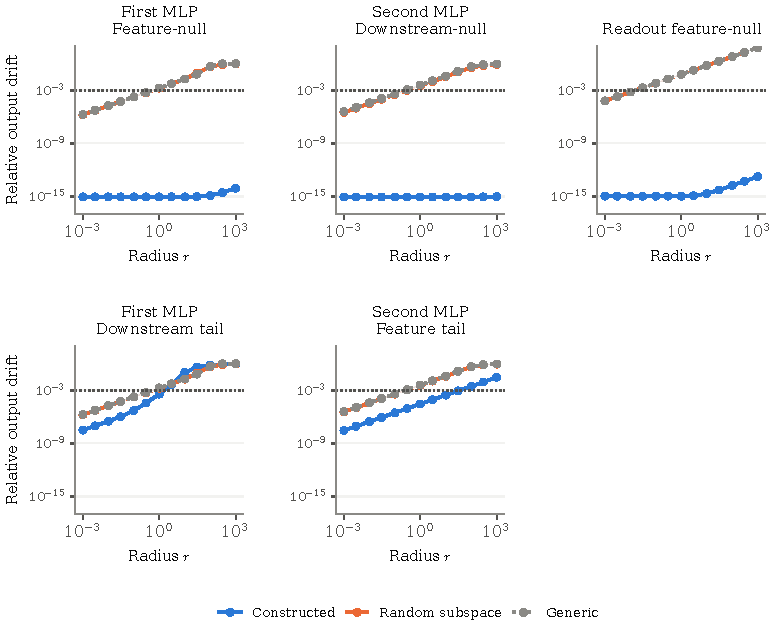
\includegraphics[width=4.670in]{vit_common_rays.pdf}
\caption{ViT common-family ray responses. Curves show the mean of within-seed median relative RMS drift; bands show one sample SD across available seeds. The horizontal line marks $10^{-3}$. Exact-family responses remain at the numerical floor. Controls use the same edited layer and normalization.}
\label{fig:vit-common-rays}\label{tab:vit-common-radii}
\end{figure}


\subsubsection{Multilayer combinations and relative-cutoff comparisons}
The compatible exact combinations preserve logits to numerical precision (Figure~\ref{fig:native-vit-sampled}b). The supplementary relative-cutoff study also finds larger sampled radii than controls for single-layer and joint approximate edits (panels a,c). Near their visibility threshold, activation changes dominate the departure from the first-order response, while mixed-weight interactions remain small (panel d).
\begin{figure}[!htbp]\centering
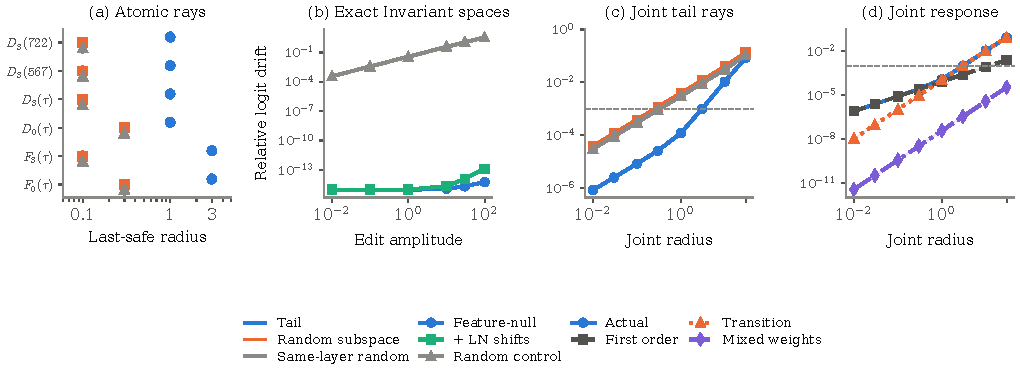
\includegraphics[width=6.122in]{vit_oceans.pdf}
\caption{ViT joint and relative-cutoff comparisons, following Appendix~\ref{app:methods-common-families}. (a) Last-safe radii for feature ($F$) and downstream ($D$) tails; subscripts identify the two MLP maps. (b) Exact compatible combinations. (c) Joint approximate edits and controls. (d) Their response decomposition. Points and bands show means and ranges of within-seed medians over 256 directions. Horizontal lines mark relative drift $10^{-3}$. Panel (a) uses dataset-RMS drift; (b--d) use median per-image relative drift. Normalizations follow Appendix~\ref{app:methods-radius}.}\label{fig:native-vit-sampled}\label{fig:c-native-approx}
\end{figure}

\subsection{Fine-tuned ResNet on RESISC45}
\label{app:resnet-common}

Every tested feature and common downstream operator has full rank, and all their approximate tails are empty at the stated cutoff. The selective construction gives one substantial exception: a 10,171-dimensional space in \texttt{layer4.2.conv2} (Table~\ref{tab:resnet-common}). These zeros concern the specified families. The full atomic kernels of the convolutional layers remain large by parameter counting, and have not been factorized in this study.

\begin{table}[!htbp]\centering
\caption{ResNet late-layer constructions. FN: feature-null; DN: additional common downstream-null; SEL: additional selective. Both marginal tails are empty in every row. The last column is only the counting lower bound $\max(0,p-45s)$ on the full atomic kernel, with $s=10,000$.}
\label{tab:resnet-common}
\small\begin{tabular}{lrrrrr}\toprule
Layer & Parameters & FN & DN & SEL & Kernel lower bound\\\midrule
\texttt{layer4.0.conv1} & 524,288 & 0 & 0 & 0 & 74,288\\
\texttt{layer4.0.conv2} & 2,359,296 & 0 & 0 & 0 & 1,909,296\\
\texttt{layer4.0.conv3} & 1,048,576 & 0 & 0 & 0 & 598,576\\
\texttt{layer4.1.conv1} & 1,048,576 & 0 & 0 & 0 & 598,576\\
\texttt{layer4.1.conv2} & 2,359,296 & 0 & 0 & 0 & 1,909,296\\
\texttt{layer4.1.conv3} & 1,048,576 & 0 & 0 & 0 & 598,576\\
\texttt{layer4.2.conv1} & 1,048,576 & 0 & 0 & 0 & 598,576\\
\texttt{layer4.2.conv2} & 2,359,296 & 0 & 0 & 10,171 & 1,909,296\\
\texttt{layer4.2.conv3} & 1,048,576 & 0 & 0 & 0 & 598,576\\
Readout & 92,205 & 0 & 0 & 0 & 0\\\bottomrule
\end{tabular}
\end{table}

The selective family comes from five low-activity channels, none entirely inactive (Table~\ref{tab:resnet-selective}).

\begin{table}[!htbp]\centering
\caption{Selective-space dimension in \texttt{layer4.2.conv2}, from the active-patch matrices. The channel indices follow the implementation's zero-based numbering.}
\label{tab:resnet-selective}
\small\begin{tabular}{rrrr}\toprule
Channel & Active patches & Rank & Nullity\\\midrule
118 & 4,164 & 4,162 & 446\\
250 & 2,335 & 2,335 & 2,273\\
275 & 992 & 992 & 3,616\\
413 & 4,059 & 4,059 & 549\\
465 & 1,321 & 1,321 & 3,287\\\midrule
Total & & & 10,171\\\bottomrule
\end{tabular}
\end{table}

The selective space preserves outputs over much larger sampled edits than generic directions (Figure~\ref{fig:resnet-common-rays}). All 256 selective probes remain below relative drift $10^{-3}$ through radius 1, while all generic probes have crossed by that radius. The sampled space contains 10,170 of the 10,171 selective directions. These measurements follow the common ray protocol and do not establish a uniform radius.

\begin{figure}[!htbp]\centering
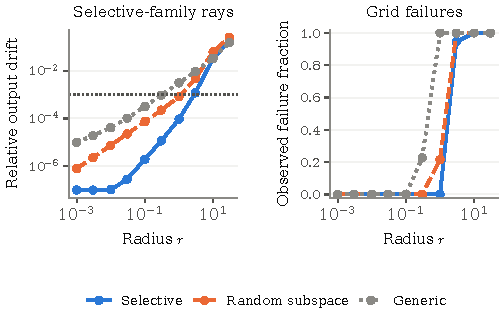
\includegraphics[width=3.024in]{resnet_common_rays.pdf}
\caption{ResNet selective-family rays, shown in the same format as the ViT study. Left: median relative RMS drift over 256 directions. Right: fraction exceeding $10^{-3}$ at any tested radius so far. Seed 0; no seed-variation band.}
\label{fig:resnet-common-rays}\label{tab:resnet-radii}
\end{figure}


\subsection{Scaling width and depth}
\label{app:scaling}\label{app:cnn-width}
The full atomic-kernel measurements on the common 10,000-image set are summarized in Figure~\ref{fig:scaling-dimensions} and Table~\ref{tab:atomic-scaling-full}. Wider networks have larger kernel fractions after 500 epochs; at matched high accuracy, the width trend is not monotonic. Increasing depth concentrates the largest fractions toward the final hidden layers. All plotted dimensions use the relative singular-value cutoff $10^{-9}$. Daggers in Table~\ref{tab:atomic-scaling-full} flag full-kernel cases with a gap below ten at this cutoff in at least one seed. Tightening the cutoff to $10^{-12}$ changes any listed per-seed fraction by at most $0.92$ percentage points. At width 512, the full ranks are only partly resolved (Appendix~\ref{app:methods-scaling}). The figure therefore shows selective-space lower bounds on the same 10,000 images as separate square markers, without connecting them to the full-kernel curves. Their epoch-500 means are $96.0\%$ in L2 and $99.8\%$ in L3.

\begin{table}[!htbp]\centering
\caption{Invariant-space dimensions as percentages of layer parameters on 10,000 analysis images: full atomic kernels, except for the selective lower bounds at width 512. Entries give means $\pm$ one sample standard deviation over three seeds at the relative singular-value cutoff $10^{-9}$. Daggers mark a full-kernel gap below ten at this cutoff in at least one seed. A dash means that the layer or milestone does not exist.}
\label{tab:atomic-scaling-full}
\small\setlength{\tabcolsep}{5pt}
\begin{tabular}{llrrrr}\toprule
Architecture & Stage & L2 & L3 & L4 & L5\\\midrule
Width 32 & High accuracy & --- & --- & --- & ---\\
 & Epoch 500 & $6.7\pm3.5$ & $27.0\pm10.0$ & --- & ---\\
Width 64 & High accuracy & $13.0\pm10.7$ & $59.5\pm11.2$ & --- & ---\\
 & Epoch 500 & $22.1\pm14.6$ & $69.5\pm2.5$ & --- & ---\\
Width 128 & High accuracy & $21.5\pm4.8$ & $47.5\pm4.4$ & --- & ---\\
 & Epoch 500 & $62.7\pm4.2$ & $90.9\pm1.9^{\dagger}$ & --- & ---\\
Width 256 & High accuracy & $17.6\pm6.1$ & $58.6\pm8.5^{\dagger}$ & --- & ---\\
 & Epoch 500 & $87.9\pm3.1$ & $98.7\pm0.0$ & --- & ---\\
Width 512 (selective) & High accuracy & $31.8\pm1.1$ & $62.4\pm0.9$ & --- & ---\\
 & Epoch 500 & $96.0\pm0.3$ & $99.8\pm0.0$ & --- & ---\\
Depth 2 & High accuracy & $75.8\pm2.9$ & --- & --- & ---\\
 & Epoch 500 & $79.9\pm1.5$ & --- & --- & ---\\
Depth 4 & High accuracy & $5.8\pm1.1$ & $28.6\pm3.1$ & $45.8\pm7.8$ & ---\\
 & Epoch 500 & $14.3\pm3.1$ & $73.4\pm2.2^{\dagger}$ & $95.2\pm0.4$ & ---\\
Depth 5 & High accuracy & $0.9\pm0.9$ & $11.4\pm2.1$ & $43.9\pm11.5$ & $57.6\pm10.0^{\dagger}$\\
 & Epoch 500 & $0.0\pm0.0$ & $37.6\pm33.0^{\dagger}$ & $91.1\pm1.5^{\dagger}$ & $96.9\pm0.7$\\
\bottomrule\end{tabular}
\end{table}


The selective-space sweep additionally covers all 60,000 training images, including width 512 (Figure~\ref{fig:scaling-detail}). It provides constructive lower bounds on the full atomic kernels on that larger set. At epoch 500, its mean L2 dimension rises from $55\%$ of layer parameters at width 128 to $94\%$ at width 512.

\begin{figure}[!htbp]\centering
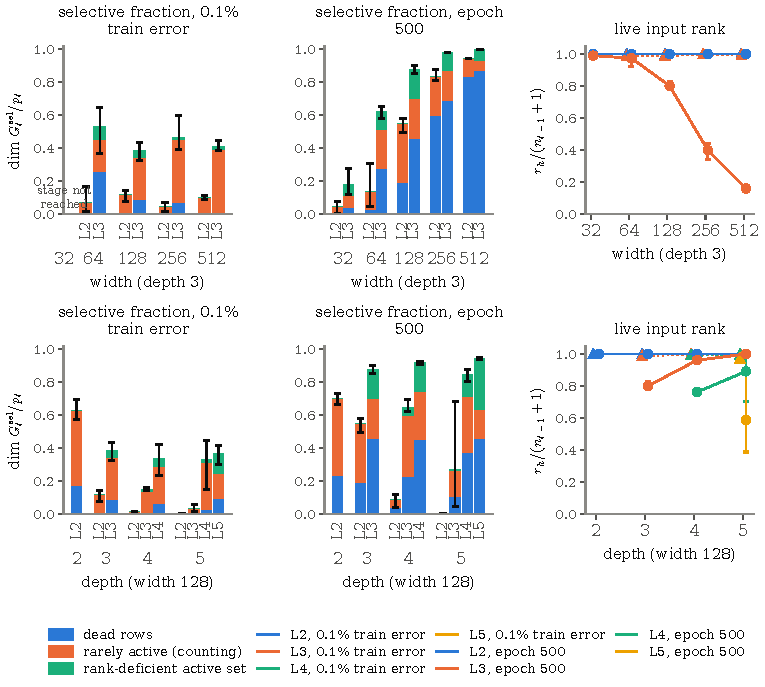
\includegraphics[width=4.588in]{paper_sweep_split.pdf}
\caption{Selective-space scaling on all 60,000 training images, complementing the full atomic-kernel measurements on 10,000 images in Figure~\ref{fig:scaling-dimensions}. Rows vary width and depth; columns show selective fractions at high accuracy and epoch 500, then normalized input-feature ranks. Bars group hidden layers in increasing order from L2. Segments separate dead rows, insufficient active-sample counts, and rank-deficient active-feature spans beyond counting. Points and whiskers show seed means and ranges; $r_h$ denotes the input-feature rank $r_\ell$.}
\label{fig:scaling-detail}
\end{figure}

The CNN sweep shows the same broad pattern: increasing width enlarges the selective ocean faster than the parameter count, even when test accuracy changes little. At half width, the selective construction leaves only readout directions. Wider models develop late convolutional channels that are active on very few images, leaving many kernel edits unconstrained. The channel-activity plot connects that observation to the measured selective dimensions. Matrix-free counts and fully assembled invariant subspace certificates are distinguished in the table.

\begin{table}[!htbp]
\caption{CNN width sweep at epoch 500. The final column is the mean selective dimension divided by parameter count. Starred cells are matrix-free selective-space dimensions without a full assembled invariant subspace certificate; the remaining cells passed numerical validation.}
\label{tab:cnn-width}
\centering
\vspace{0.45em}
\begin{tabular}{lrrrrrr}
\toprule
network & params & test acc. & seed 0 & seed 1 & seed 2 & ocean/params \\
\midrule
$0.5\times$ & $13{,}922$ & $.990$--$.992$ & $1{,}080$ & $430$ & $620$ & $0.051$ \\
base & $45{,}114$ & $.994$--$.995$ & $3{,}803$ & $8{,}782$ & $5{,}565$ & $0.134$ \\
$2\times$ & $159{,}338$ & $.994$--$.995$ & $45{,}493$ & $64{,}416^{*}$ & $45{,}004^{*}$ & $0.324$ \\
\bottomrule
\end{tabular}
\end{table}
\begin{figure}[!htbp]\centering
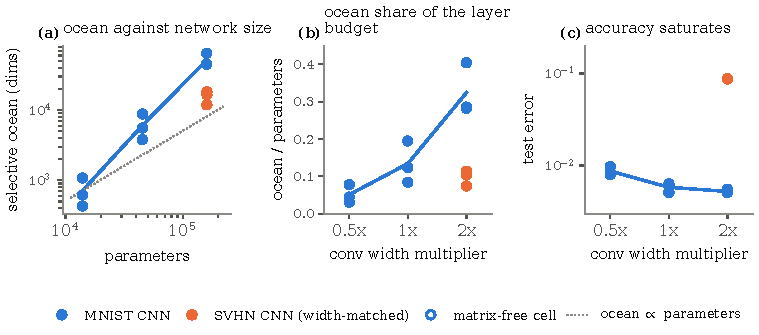
\includegraphics[width=4.553in]{width_scaling.pdf}\par\smallskip
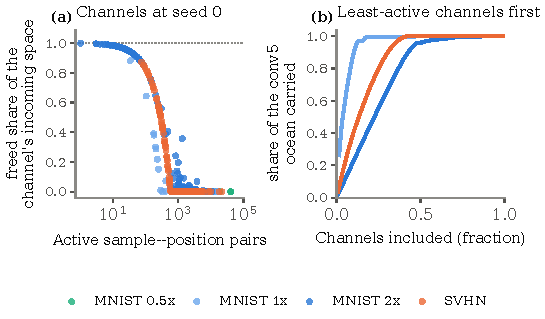
\includegraphics[width=3.268in]{width_channels.pdf}
\caption{CNN width scaling (top) and conv5 channel activity (bottom, seed 0). Selective dimensions grow faster than parameter count while accuracy changes little. Hollow markers denote matrix-free dimensions without assembled certificates; orange points compare the width-matched SVHN CNN. The least-active channels carry most of the conv5 selective space. At half width that space is empty.}\label{fig:early-draft-cnn-width}
\end{figure}

Dimension and radius need not scale together. Figure~\ref{fig:radius-sweeps} compares first gate crossings and first visible output changes on the width/depth slices. Neither radius follows a simple monotone law in these seed-0 measurements. The gap between crossing a boundary and changing outputs remains important when interpreting a larger ocean dimension.
\begin{figure}[!htbp]\centering
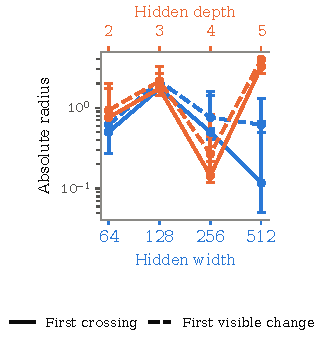
\includegraphics[width=1.954in]{square_sweeps.pdf}
\caption{Radius versus MLP width (blue, bottom axis) and hidden depth (orange, top axis). Solid lines mark first gate crossings and dashed lines the first output change above $10^{-3}$. Points are medians over sampled slice angles; whiskers span the 10th--90th percentiles. Each architecture uses seed 0 at its tested checkpoint.}\label{fig:radius-sweeps}
\end{figure}

\subsection{Inside the co-occurrence deficit}
\label{app:mechanism}

The deficit measures constraints missing from the observed feature--downstream pairings. We first examine the contribution of selective units, whose exact inactive-side construction uses ReLU's zero slope, then ask how the deficit relates to sample clustering and neural collapse. The grouping and shuffle protocols are defined in Appendix~\ref{app:methods-branches}. Pairing-shuffle results use ReLU seed 0; the clustering comparisons also include leaky ReLU and GELU.

\subsubsection{Selective units and cross-unit cancellations}
Selective units create invariant directions when their active input features leave incoming parameter directions unconstrained. Their contribution can therefore be large even without class-aligned clusters. The full width and depth trajectories and the within-unit decomposition appear in Appendix~\ref{app:atomic}; Figure~\ref{fig:early-draft-mechanism-family} compares their relation to the atomic kernels across model families. In fitted ReLU networks, selective directions account for much of the hidden kernel. Leaky ReLU gives a useful contrast: its nonzero negative-side slopes require cancellations across units.

\begin{figure}[!htbp]\centering
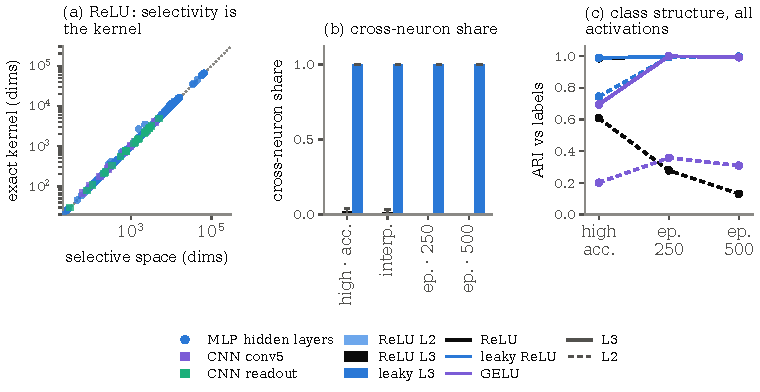
\includegraphics[width=4.558in]{deficit_mechanisms.pdf}
\caption{Selective and cross-neuron mechanisms across architectures and activations. (a) Selective dimensions against numerical atomic dimensions across measured ReLU widths, depths and CNN layers. (b) Cross-neuron fractions, median and range across seeds. (c) Agreement between clusters of similar downstream maps and the digit labels, measured by the adjusted Rand index: 1 means identical partitions, and 0 is the chance baseline. This panel measures class agreement, not kernel size or the fraction of deficit explained.}\label{fig:early-draft-mechanism-family}
\end{figure}

\begin{table}[!htbp]\centering
\caption{Leaky-ReLU mechanism check, width 128, seed 0 at high accuracy. Selective candidates use the hard activity mask; the additional condition $V_{\mathrm{lin}}^0 A_L\bar h_{L-1,i}^0=0$ for every sample accounts for the nonzero negative-side response. The retained candidate count is compared with the measured numerical kernel.}
\small\begin{tabular}{lrrr}\toprule
Layer & Selective candidates & After readout condition & Atomic kernel\\\midrule
L3 & 6,311 & 5,021 & 5,036\\\bottomrule
\end{tabular}\end{table}

\subsubsection{Sample clustering and missing pairings}
For a partition $\mathcal G$, let $H_G$ be the span of the augmented features in group $G$ and $C_G$ the span of the downstream-map rows in that group. Let $r_h$ and $r_d$ be their respective ranks over all samples, and define $\mathcal P(\mathcal G)=\sum_{G\in\mathcal G}H_G\otimes C_G$. The deficit separates as
\[
 \delta=r_hr_d-\operatorname{rank}J_\ell
 =\underbrace{r_hr_d-\dim\mathcal P(\mathcal G)}_{\text{missing across groups}}
 +\underbrace{\dim\mathcal P(\mathcal G)-\operatorname{rank}J_\ell}_{\text{missing within groups}}.
\]
For a positive deficit $\delta>0$, the explained share is the first term divided by $\delta$. It quantifies how much of the deficit follows from separating samples into these groups. Purity instead measures whether the groups agree with class labels. A class-pure partition can therefore explain little of the rank deficit. Appendix~\ref{app:methods-branches} defines purity and its matched random-label control.


In the three-hidden-layer, width-128 MNIST ReLU MLP, class groups explain an increasing share of the L3 deficit during training, while their L2 share remains zero. Figure~\ref{fig:cluster-stages}  shows the complete five-stage trajectories for all three seeds. This is a comparison between layers of one architecture; the corresponding clustering measurements across network depths have not yet been completed.
\begin{figure}[!htbp]\centering
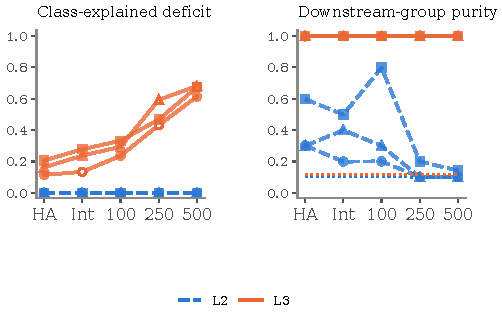
\includegraphics[width=3.013in]{cluster_relu_stages.pdf}
\caption{Class organization in the width-128 ReLU MLP across five fitted stages. Left: share of the deficit explained by class groups. Right: label purity of ten requested downstream k-means groups; dotted lines give matched random-label purity. Markers distinguish seeds 0--2. Open markers flag tolerance-sensitive partition ranks. HA and Int denote high accuracy and interpolation.}\label{fig:cluster-stages}
\end{figure}
\FloatBarrier




Figure~\ref{fig:mechanism} shows grouping and shuffle tests of the ReLU co-occurrence deficit. Finer downstream groups can explain all of the ReLU L3 endpoint deficit, while matched random groups explain little. A global shuffle retains about two thirds of that deficit, whereas a shuffle restricted to classes retains almost all of it. In L2, both shuffles retain essentially the full deficit. 

\begin{figure}[!htbp]
\centering
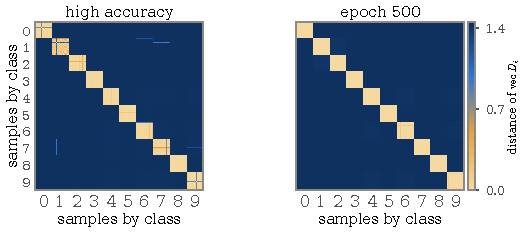
\includegraphics[width=3.146in]{dmap_pca.pdf}
\caption{Pairwise distances between unit-normalized L3 downstream maps (ReLU width 128, seed 0; 500 samples ordered by class). Sand denotes small distances and navy large distances. The ten class groups become more uniform by epoch 500.}
\label{fig:dmap-pca}
\end{figure}
\begin{figure}[!htbp]\centering
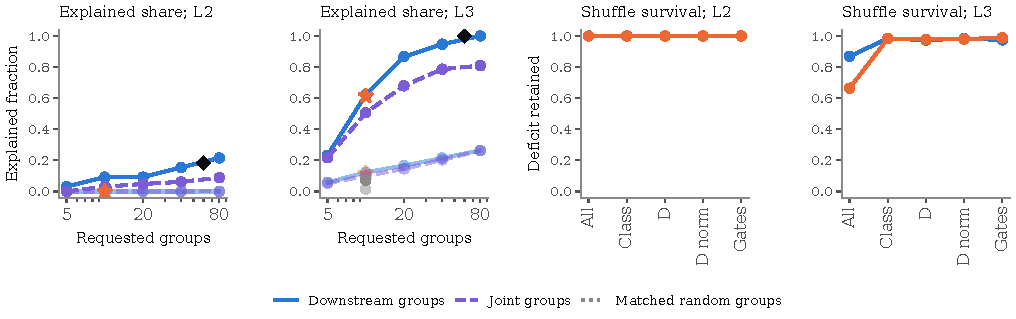
\includegraphics[width=6.098in]{cluster_pairings.pdf}
\caption{Grouping and pairing tests in the width-128 ReLU MLP, seed 0. Left pair: deficit explained as the requested group count changes; light and dark curves denote high accuracy and epoch 500. Stars mark class groups and diamonds suffix-gate patterns, at their actual group count. Right pair: deficit remaining after global shuffles (All) or shuffles within classes, downstream groups (D), normalized downstream groups (D norm), or suffix-gate groups; blue is high accuracy and orange epoch 500. The L2 deficit survives almost entirely; L3 is more sensitive to global shuffling than to shuffling within groups.}\label{fig:mechanism}
\end{figure}
\FloatBarrier


The distance-threshold analysis groups downstream maps that are close in both direction and magnitude. It uses the common normalization and complete-linkage rule from Appendix~\ref{app:methods-branches}: each group has normalized diameter at most $\varepsilon$. We apply the same threshold grid at each training stage and compare group purity with shuffled-label controls of the same sizes.

Table~\ref{tab:dmap-threshold} shows the L3 results at one common threshold. The late-training groups are nearly class-pure and contain multiple samples; the matched random-label purity is about $0.11$. GELU needs many more groups at high accuracy to satisfy the same distance threshold. Thus the downstream maps become concentrated into a smaller number of class-aligned groups as training proceeds. L2 behaves differently: ReLU and GELU retain overlapping within-class and between-class distance distributions, while leaky ReLU becomes class-separated. These distance measurements describe concentration; the rank decomposition above separately measures its relation to the deficit.

\begin{table}[!htbp]\centering
\caption{L3 downstream groups at normalized diameter threshold $\varepsilon=1.0$, width-128 MNIST MLP, seed 0. Each cell gives number of groups / purity.}
\label{tab:dmap-threshold}
\begin{tabular}{lccc}\toprule
Activation & High accuracy & Epoch 250 & Epoch 500\\\midrule
ReLU & $24/0.997$ & $11/0.998$ & $11/0.999$\\
Leaky ReLU & $24/0.996$ & $10/0.998$ & $10/0.998$\\
GELU & $114/0.998$ & $10/1.000$ & $15/1.000$\\\bottomrule
\end{tabular}
\end{table}





\begin{figure}[!htbp]\centering
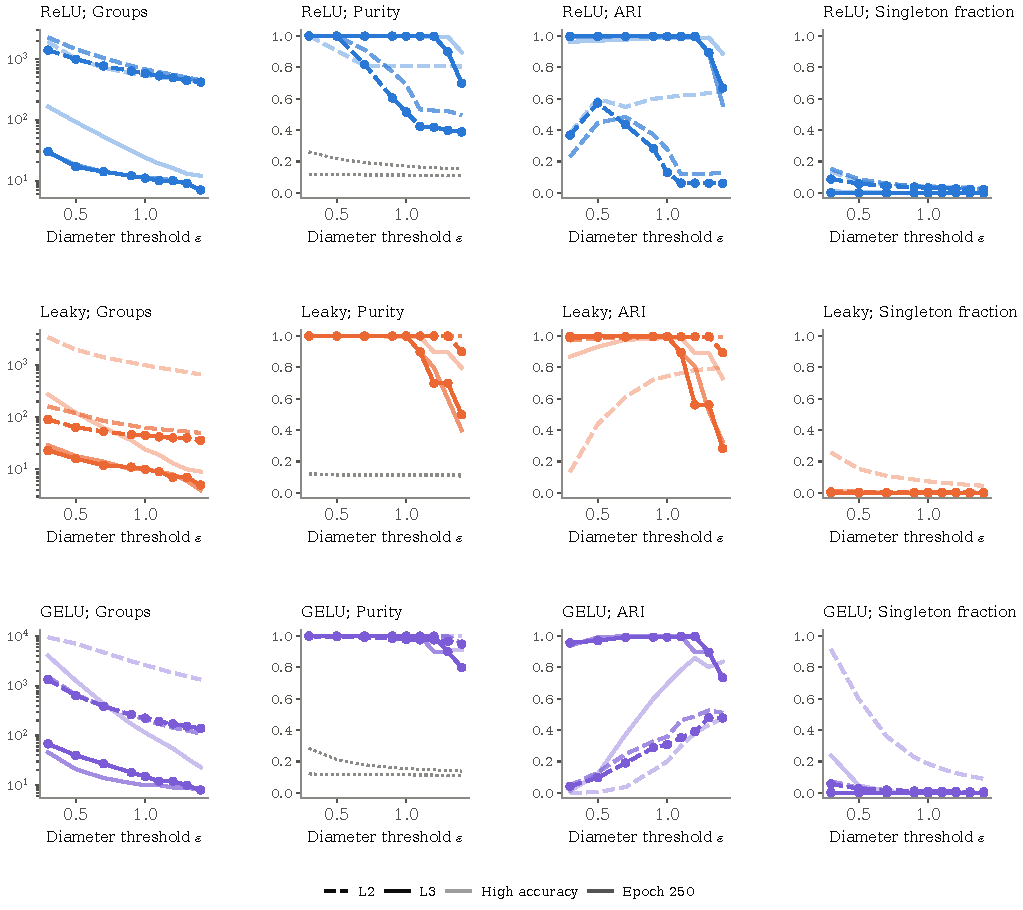
\includegraphics[width=6.138in]{cluster_diameters.pdf}
\caption{Diameter-controlled clustering in the same width-128 networks, seed 0. Rows compare activations; columns show group count, label purity, adjusted Rand index and the fraction of samples in singleton groups. Solid and dashed curves denote L3 and L2. Opacity increases from high accuracy to epoch 250 and epoch 500; endpoint curves have markers. Dotted purity controls shuffle labels at fixed group sizes. L3 forms class-aligned groups for every activation, whereas L2 behavior depends on activation. High purity carried by singletons is distinguished from grouping whole classes.}\label{fig:cluster-diameters}
\end{figure}
\FloatBarrier


Figure~\ref{fig:cluster-diameters} compares both layers at every measured stage. Unlike a fixed ten-group partition, this rule allows more groups when the maps require them. It also reports the fraction of samples in singleton groups, since high purity from isolated samples would provide little evidence of class organization. The adjusted Rand index compares the group and class assignments through sample pairs, correcting for chance agreement: one indicates matching partitions and values near zero indicate chance-level agreement.

Figure~\ref{fig:cluster-seeds} extends the L3 endpoint comparison to all three training seeds using the same diameter grid and normalization. The additional seeds cover epoch 500, while the stage and layer comparisons above retain their original coverage.
\begin{figure}[!htbp]\centering
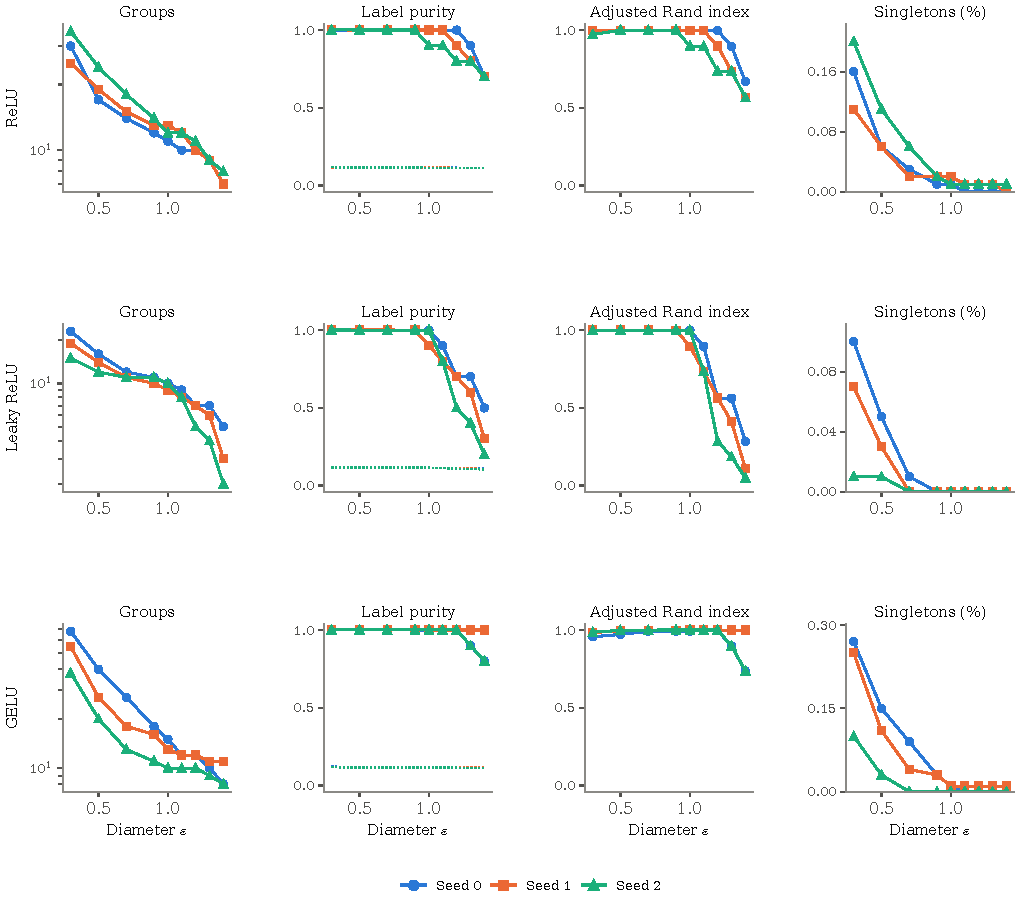
\includegraphics[width=6.120in]{clustering_seeds.pdf}
\caption{Diameter-controlled downstream clustering across seeds 0--2 in width-128 MNIST MLPs, L3 at epoch 500. Rows compare activations; columns show group count, label purity, adjusted Rand index and the percentage of samples in singleton groups. Colors and markers identify seeds; dotted purity curves give matched-size shuffled-label means. All seeds use the same analysis size, distance normalization and diameter grid.}\label{fig:cluster-seeds}
\end{figure}
\FloatBarrier



\subsubsection{Neural collapse and class organization}
\label{app:nc}


Neural collapse describes a collection of geometric patterns that can emerge in a classifier's final features during training: within-class features concentrate, class means approach a regular simplex, classifier weights align with those means, and classification approaches the nearest-class-mean rule \citep{papyan2020collapse}. We use measurements of these patterns to ask whether class organization of the features accompanies class organization of the downstream maps.


Figure~\ref{fig:nc-full} follows the measured width-128 MNIST ReLU, leaky-ReLU and GELU models, with an identity-activation control. NC1 compares within-class feature variance with between-class variance. The two NC2 measurements quantify variation in class-mean norms and departure of their normalized Gram matrix from an equiangular tight frame. The plotted NC4 diagnostic is the disagreement between nearest-class-mean predictions and labels. All three nonlinear families develop concentrated features during training, although the strength and subsequent evolution depend on activation and layer. The identity control does not show comparable concentration, and these measurements do not establish every neural-collapse property in every architecture.



\begin{figure}[!htbp]
\centering
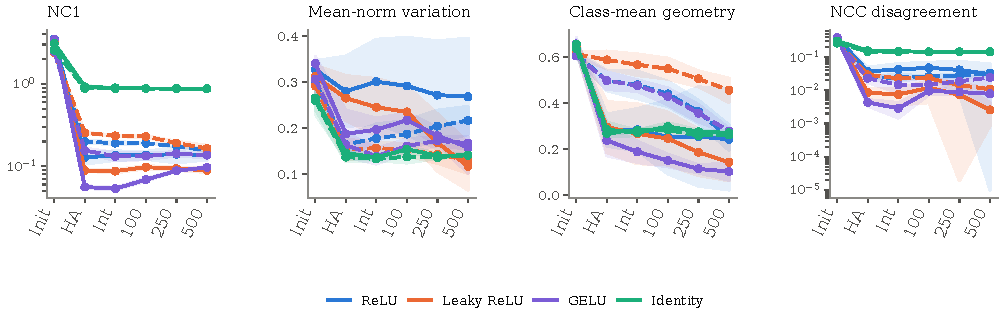
\includegraphics[width=6.022in]{nc_full_sd.pdf}
\caption{Neural-collapse measurements across training, seed means with one sample standard deviation shaded. Solid lines show L3; dashed lines show L2. Bands summarize up to three seeds at each measured stage and use a positive plotting floor of $10^{-5}$ on logarithmic axes.}
\label{fig:nc-full}
\end{figure}


Feature concentration and downstream-map organization can develop together during training. Figure~\ref{fig:nc-pairings} compares inverse NC1 with downstream class separation and label purity at matching checkpoints, separately for L2 and L3. Larger inverse NC1 means stronger feature concentration. The comparisons describe co-occurrence, with variation across activations and layers. They do not establish that either phenomenon causes the other or causes the co-occurrence deficit: downstream maps also depend on later weights and activation slopes. These observations motivate studying the two forms of organization together.

\begin{figure}[!htbp]\centering
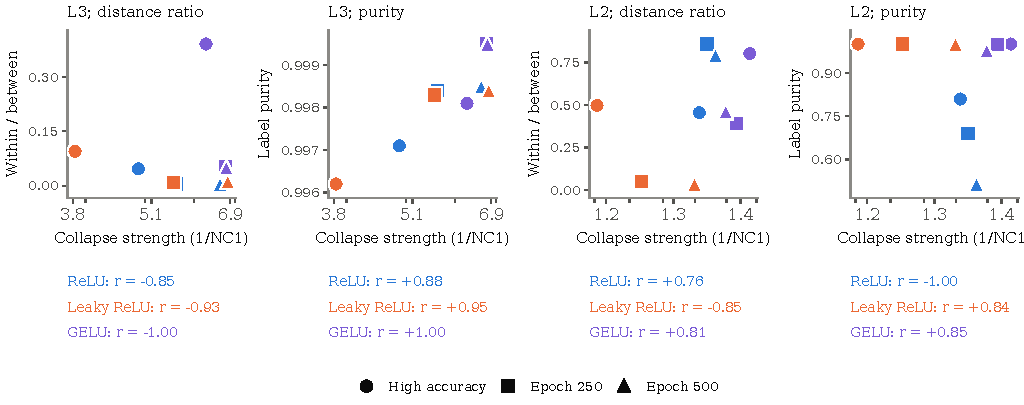
\includegraphics[width=6.147in]{nc_pairings.pdf}
\caption{Feature concentration versus downstream clustering in width-128 MNIST MLPs, seed 0. Larger $1/\mathrm{NC1}$ means stronger input-feature collapse; the horizontal scale is logarithmic. Points compare within-class/between-class downstream-map distance or diameter-cluster label purity at $\varepsilon=1$, at three matched checkpoints. Left pair: L3 maps and L2 features; right pair: L2 maps and L1 features. Colors identify activations and marker shapes identify stages. Each panel reports the within-activation Pearson correlation with $\log_{10}(1/\mathrm{NC1})$, using only these three points; a constant response has undefined correlation. These descriptive correlations do not establish a causal relationship.}\label{fig:nc-pairings}
\end{figure}
\FloatBarrier


\subsection{Dependence on training and evaluation data}
\label{app:data-dependence}
Data affect ocean geometry in two distinct ways. Changing the training set changes the learned weights and representations. Changing the evaluation set holds the network fixed and changes the constraints defining its invariant directions. We study these effects separately below.

\subsubsection{Training data}
\label{app:training-data}
Training on more images changes the learned representation as well as the number of fitting constraints. We compare models trained from initialization on progressively larger subsets with a model trained on the complete training set, evaluating both on the same smaller subsets. ``Train on $n$'' in the figures denotes the former; ``Full-data, $n$ constraints'' denotes the latter. The architecture and optimization recipe are held fixed, and geometry probes leave the input layer unchanged.

At the smallest matched evaluation set, the model trained on all images has substantially larger hidden atomic kernels than the model trained only on that subset. Training on more data can therefore create a representation with more invariant directions, even though adding evaluation constraints to a fixed representation removes directions. The reduced-data training sweep is not monotone in sample size, so this comparison does not imply a universal growth law.


\begin{figure}[!htbp]\centering
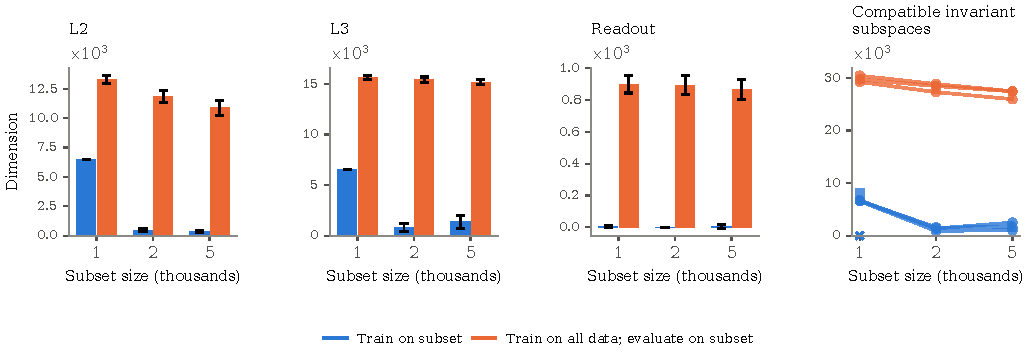
\includegraphics[width=6.156in]{data_dimensions_four.pdf}
\caption{Dimensions at epoch 500 versus subset size, width-128 ReLU MLPs. Colors distinguish subset-trained and full-data networks throughout. First three panels: total atomic dimensions, with seed means and sample-standard-deviation whiskers. Fourth: compatible invariant subspace dimensions, with one curve per seed; solid/circles denote bottom-up construction, dashed/squares top-down, and dotted/crosses the atomic sum. Zero means no validated direction, including a failed certificate. Unmeasured constructions have no point. L1 is fixed.}\label{fig:data-atomic}\label{fig:data-branches}
\end{figure}
\FloatBarrier


The small-subset models show why single-layer invariant directions must be checked before combining them. With few samples, the number of output constraints alone can force large hidden atomic kernels, even when the feature and downstream spans have full rank. Each atomic edit preserves the frozen outputs when applied alone. Simultaneous edits can change those outputs through interactions between layers. The rightmost panel of Figure~\ref{fig:data-atomic} compares compatible dimensions across sample counts and construction orders. 




Table~\ref{tab:subset-order} gives a concrete example at $N=1{,}000$. The two hidden atomic kernels each have 6,512 directions, yet their full sum fails the invariant subspace check. Bottom-up construction keeps the L2 space and restricts L3; top-down construction does the reverse. Their different totals show that layer order affects how many simultaneously invariant directions the construction retains.
\begin{table}[!htbp]\centering
\caption{Compatibility in the 1,000-sample retraining, seed 0. The input layer is fixed. The atomic sum is a tangent space but fails the invariant subspace check.}\label{tab:subset-order}
\begin{tabular}{lrrrr}\toprule
Construction & L2 & L3 & readout & total\\\midrule
Atomic sum &6512&6512&10&13034\\
Bottom-up &6512&197&10&6719\\
Top-down &1477&6512&10&7999\\\bottomrule
\end{tabular}\end{table}

The radius measurements separate changes in the first gate crossing from changes in output visibility. In the subset-trained models, the first crossing moves outward as training-set size grows, while the visible radius changes much less. Excluded-image responses are already nonzero in the frozen model and decrease as more images constrain the directions. The summary and absolute-radius curves below compare both training conditions.

The upper-middle panel of Figure~\ref{fig:early-draft-subset-rays} shows the first sampled radius at which the output change exceeds $10^{-3}$ times the base output norm. Several seed curves coincide because the scan uses a discrete radius grid; equal plotted values mean the threshold was reached at the same tested radius. The lower-left panel follows invariant subspace directions constructed on 1,000 images. Outputs on those fitted images remain near numerical zero over the initial part of the scan, while excluded-image outputs change immediately. This separation shows which invariance depends on the fitted sample set. Colors distinguish subset training from a full-data network throughout the figure. In the upper row, solid and dashed lines denote invariant subspace and generic rays; in the lower-left panel they denote fitted and excluded images.


\begin{figure}[!htbp]\centering
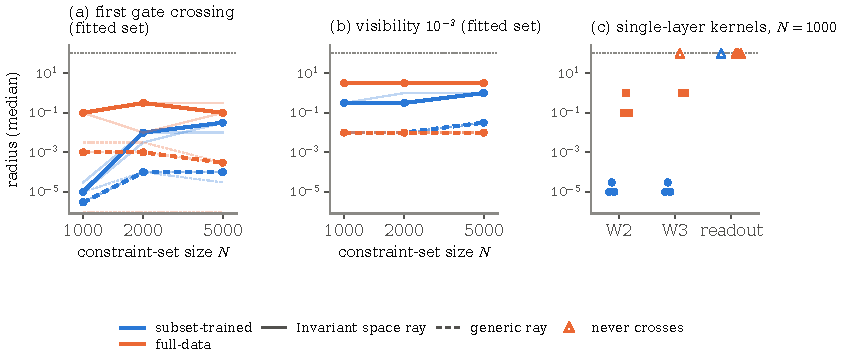
\includegraphics[width=5.057in]{p1_radii_consistent.pdf}\par\smallskip
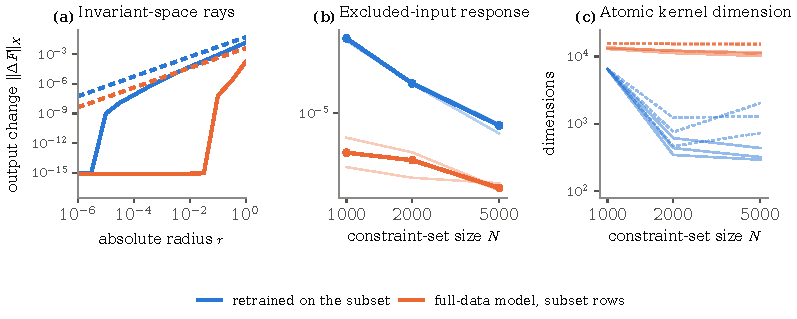
\includegraphics[width=4.780in]{p1_exposure_consistent.pdf}
\caption{Reduced-sample geometry across three seeds, with the input layer fixed. Top: fitted-set first crossing, $10^{-3}$ relative output visibility, and single-layer probes at $N=1{,}000$; markers summarize 128 directions and triangles mark censoring. Bottom: fitted versus excluded response, excluded response at matched radius, and hidden atomic dimensions. Retraining and analysis-set restriction are kept separate. Cap-limited input-layer measurements give $\rank J_1\ge16{,}512$ and $\dim K_1\le16{,}384$; they are excluded from the probes.}\label{fig:early-draft-subset-rays}
\end{figure}


\begin{figure}[!htbp]\centering
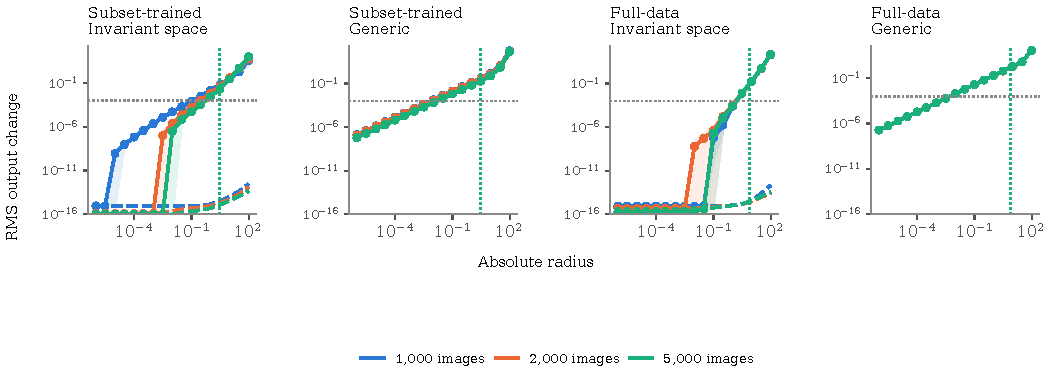
\includegraphics[width=6.313in]{data_rays_four.pdf}
\caption{Absolute-radius invariant subspace and generic probes at epoch 500, for subset-trained networks (left pair) and full-data networks evaluated on the same subsets (right pair). Colors denote subset size. Solid/dashed lines show actual/frozen response; means and ranges summarize three seed medians. L1 is fixed. Vertical dotted lines mark one tenth of the network norm; the horizontal line marks output change $10^{-3}$.}
\end{figure}
\FloatBarrier



\subsubsection{Evaluation data at a fixed network}
\label{app:newbatch}

How much of an ocean survives when the same trained network is evaluated on more images? We hold its parameters fixed and add either a disjoint training batch or test images to the original analysis set. Every new image adds constraints, so the original kernel can only shrink. The question is how much of its invariance was specific to the original images.

The hidden-layer kernels largely survive the additional constraints, including when the analysis set is doubled. The full-training-set selective measurements in Appendix~\ref{app:atomic} also remain substantial. The input layer behaves differently: the measured reference-model kernel disappears on the larger evaluation set. Thus the persistence of hidden directions is not a consequence of every layer being insensitive to new images. Figure~\ref{fig:newbatch} shows the dimension trajectories at epoch 500.


Table~\ref{tab:newdata-main} separates additional training images from unseen test images at three checkpoints. Each model was trained on all 60,000 MNIST training images; the initial analysis set contains 10,000 of them. Both additions remove a smaller fraction of the hidden kernels at epoch 500 than at the earlier fitted stages.
\begin{table}[!htbp]
\centering
\caption{Atomic-kernel dimensions removed by adding 10,000 images to the 10,000-image analysis set. Width-128 ReLU MLP; percentages of the original kernel, with ranges over three seeds. The network is fixed within each comparison. \emph{Training} means additional images seen during training but absent from the initial analysis set; \emph{test} means unseen images.}
\label{tab:newdata-main}
\small\setlength{\tabcolsep}{4pt}
\begin{tabular}{llrr}
\toprule
Stage & Added images & L2 & L3\\
\midrule
High accuracy & Training & $16$--$32\%$ & $4.7$--$7.7\%$\\
 & Test & $16$--$30\%$ & $6.2$--$11.4\%$\\
Interpolation & Training & $18$--$27\%$ & $3.9$--$6.3\%$\\
 & Test & $16$--$26\%$ & $5.3$--$10.0\%$\\
Epoch 500 & Training & $4.0$--$6.2\%$ & $1.0$--$1.4\%$\\
 & Test & $3.7$--$5.6\%$ & $2.1$--$2.9\%$\\
\bottomrule
\end{tabular}
\end{table}

\paragraph{From clean inputs to pure noise.}
\label{app:newinput-interpolation}
We measure how much of each atomic space survives when clean MNIST inputs are gradually replaced by uniform noise, following Appendix~\ref{app:methods-newinput}. Most hidden-layer directions survive throughout. Intermediate mixtures constrain the spaces more than pure noise, while the readout loses a larger and more seed-dependent fraction (Figure~\ref{fig:newinput-shift}). Thus moving farther from the training distribution need not remove more invariant directions.

\begin{figure}[!htbp]\centering
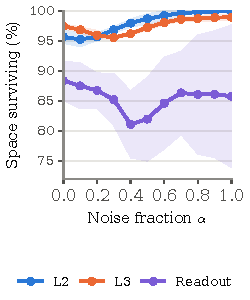
\includegraphics[width=1.499in]{newinput_interpolation.pdf}
\caption{Atomic-space survival under clean-to-noise interpolation, mean $\pm$ sample SD across three seeds. L3 has additional rank-cutoff sensitivity (Appendix~\ref{app:methods-newinput}), which preserves the qualitative trend.}
\label{fig:newinput-shift}
\end{figure}

\paragraph{SVHN inputs.}
Most of the hidden-layer spaces also survive SVHN images passed through the fixed MNIST preprocessing (Table~\ref{tab:newinput-svhn}). L2 survival is higher than for the clean MNIST reference in every seed; L3 and readout effects vary across seeds. Survival therefore depends on the additional feature and downstream constraints, rather than distribution shift alone.
\begin{table}[!htbp]\centering
\caption{Atomic-space survival (\%), mean $\pm$ sample SD across three seeds. SVHN uses the fixed MNIST representation. Rank sensitivity is assessed separately from seed variation.}
\label{tab:newinput-svhn}
\small\begin{tabular}{lccc}\toprule
Added inputs & L2 & L3 & Readout\\\midrule
Clean MNIST & $95.63 \pm 1.07$ & $97.39 \pm 0.42$ & $88.33 \pm 3.30$\\
SVHN & $98.41 \pm 0.91$ & $97.20 \pm 0.58$ & $87.30 \pm 3.04$\\\bottomrule\end{tabular}\end{table}



\begin{figure}[!htbp]\centering
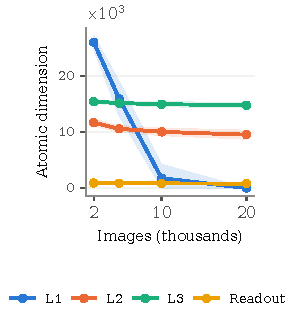
\includegraphics[width=1.776in]{evaluation_dimensions.pdf}
\caption{Atomic dimensions as more evaluation images constrain the same width-128 MNIST ReLU network at epoch 500. Lines show means over seeds 0 and 1; bands show one sample standard deviation. Every layer has measurements on the same evaluation-size grid.}\label{fig:newbatch}
\end{figure}
\FloatBarrier


On smaller analysis subsets, directions invariant on the fitted images can already change excluded-image outputs before any gate switches. The fitted/excluded response comparisons in Figure~\ref{fig:early-draft-subset-rays} make this dependence on the evaluation set explicit. A frozen certificate on one set of images need not extend to another.


\subsection{Kernel persistence}
\label{app:persistence}\label{app:persistence-newdata}
The ReLU ocean grows through training while retaining most of its earlier invariant directions. This is stronger than observing a large kernel at each checkpoint: the spaces remain substantially aligned as learning changes the weights. Removing directions supported on dead-unit coordinates leaves much of the same persistence, so the effect extends to directions involving active units.

Figures~\ref{fig:persistence}--\ref{fig:persistence-angles} compare all measured fitted-stage pairs in the reference ReLU, leaky-ReLU and GELU models. They separate retained mass, effective lost dimension and output sensitivity of the part that becomes visible. The principal-angle distributions show that ReLU's geometric loss is concentrated in a small part of the space. Many lost directions also have weak downstream output sensitivity, although a few late L2 comparisons have larger gain than generic directions. Geometric retention and functional exposure are therefore distinct measurements.

The activation comparisons qualify the persistence claim. Leaky-ReLU kernels rotate more substantially late in training, whereas GELU's late numerical kernels retain substantial projected mass but lack a stable exact-rank interpretation. These results show that strong ReLU persistence is a property of the learned geometry, not a consequence of the definition of a kernel.

\begin{figure}[!htbp]\centering
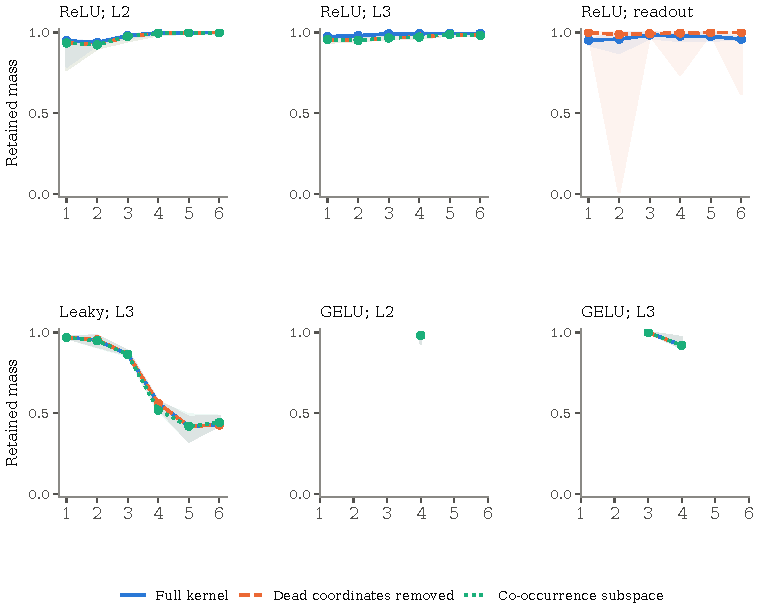
\includegraphics[width=4.560in]{persistence_summary_part1.pdf}
\caption{Checkpoint persistence in width-128 MNIST MLPs: retained mass. Pair indices 1--6 denote HA$\to$Int, Int$\to$100, 100$\to$250, 250$\to$500, HA$\to$500 and Int$\to$500; HA and Int are high accuracy and interpolation. Curves show medians and ranges across three seeds. Empty spaces have no retention value; unresolved component splits are omitted. GELU kernels remain cutoff-dependent.}\label{fig:persistence}
\end{figure}
\begin{figure}[!htbp]\centering
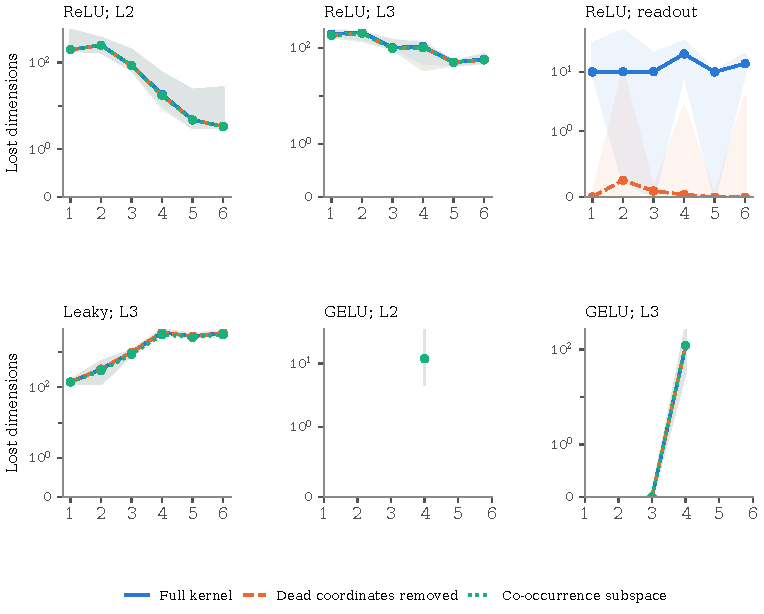
\includegraphics[width=4.583in]{persistence_summary_part2.pdf}
\caption{Effective lost dimension, with the checkpoint pairs and conventions of Figure~\ref{fig:persistence}. The vertical scale is linear near zero and logarithmic above it.}\label{fig:persistence-lost}
\end{figure}
\begin{figure}[!htbp]\centering
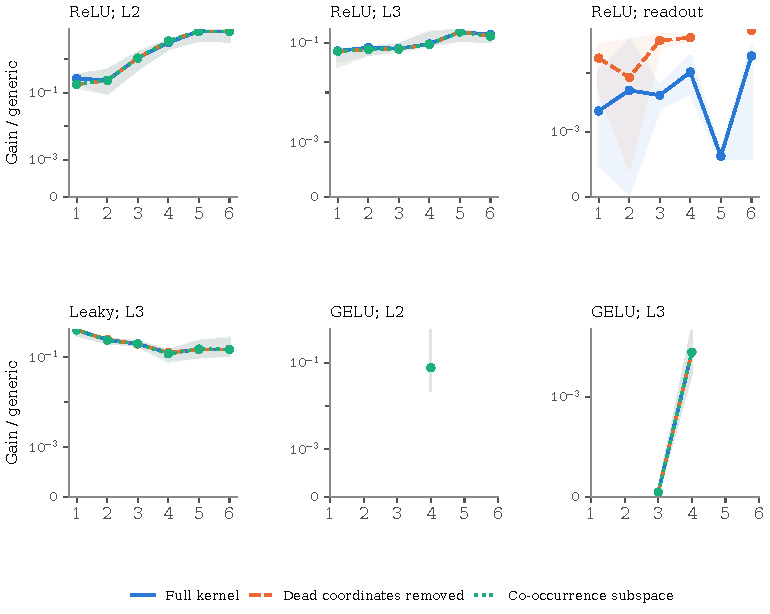
\includegraphics[width=4.620in]{persistence_summary_part3.pdf}
\caption{Output gain of lost components relative to generic directions, with the conventions of Figure~\ref{fig:persistence}.}\label{fig:persistence-gain}
\end{figure}
\begin{figure}[!htbp]\centering
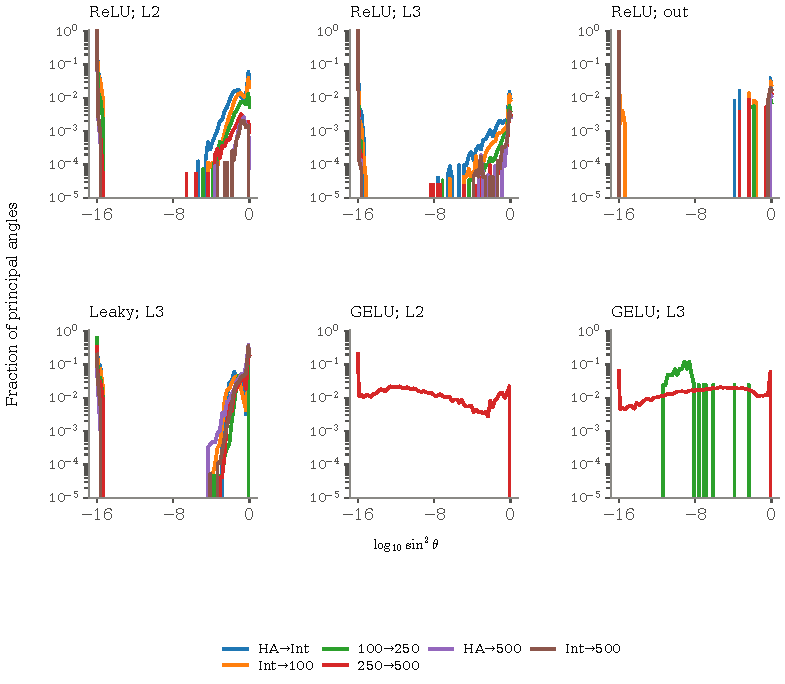
\includegraphics[width=4.710in]{persistence_angles.pdf}
\caption{Principal-angle distributions for the same checkpoint pairs, normalized within each seed and then averaged. ReLU retains a large aligned component, while leaky ReLU rotates more substantially late in training.}\label{fig:persistence-angles}
\end{figure}
\FloatBarrier


Figure~\ref{fig:persistence-tails} places this alignment alongside dimension growth. The later kernel can contain many new directions even when it retains most of the earlier one. Approximate directions with smaller singular values also tend to align more strongly with the next checkpoint's kernel. These are projected-mass comparisons, not counts of directions proved to become exactly invariant. All comparisons use checkpoint endpoints; they do not specify how the kernel moves continuously between them. Parent--sibling intersections are reported with the connectivity application in Appendix~\ref{app:lmc}.

\begin{figure}[!htbp]\centering
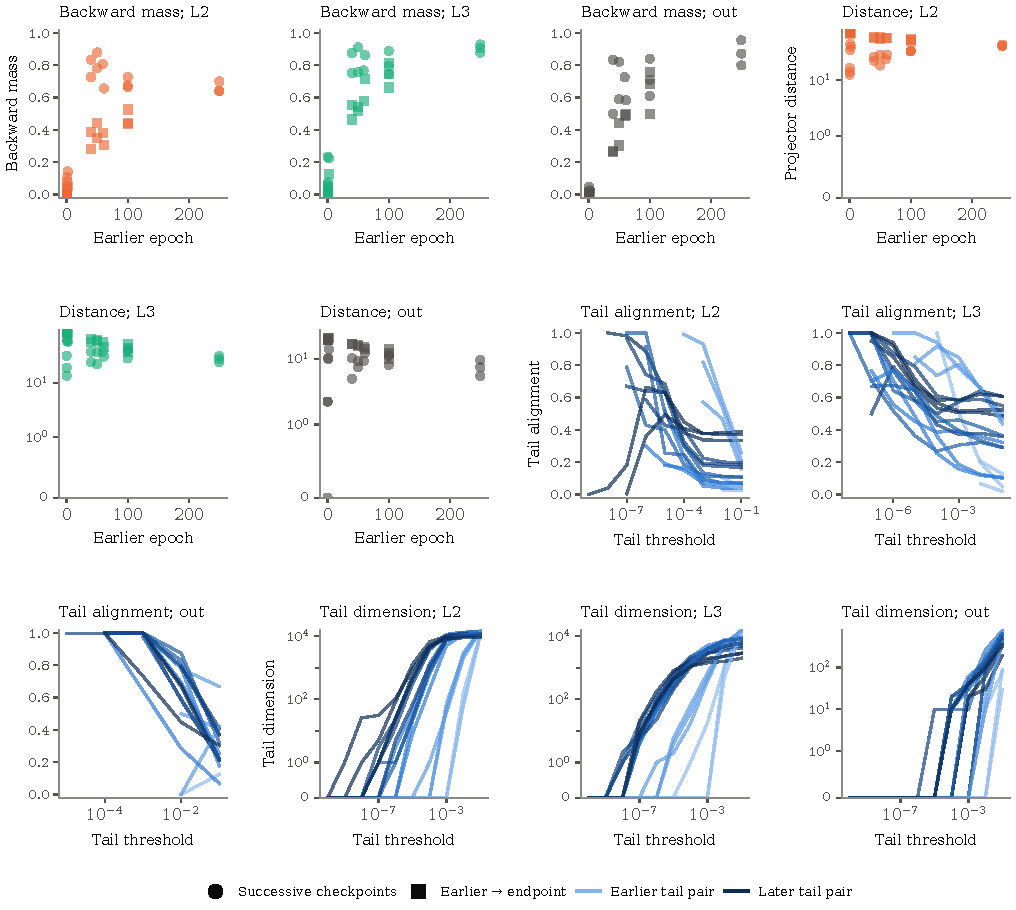
\includegraphics[width=6.096in]{persistence_tails.pdf}
\caption{Growth and spectral-tail alignment in the width-128 ReLU MLP, all three seeds. Panels 1--3 show how much of the later kernel was already present earlier; panels 4--6 show the projector distance, for every recorded checkpoint pair. Panels 7--9 and 10--12 show the positive spectral tail, excluding the current numerical kernel: its mean squared projection into the next kernel and its dimension, over the complete threshold grid on $J/\sqrt{s}$. Each line is one seed and consecutive checkpoint pair; darker lines denote later pairs. Alignment is projected mass, not an exact intersection dimension.}\label{fig:persistence-tails}
\end{figure}
\FloatBarrier


The component diagnostics in Figure~\ref{fig:persistence-diagnostics} distinguish two ways a direction can survive: it can remain invisible on active coordinates, or become supported on coordinates that are dead later. They also locate the lost mass within the later Jacobian spectrum and report the later sensitivity of sampled kernel and tail directions. For GELU, Table~\ref{tab:persistence-gelu-tau} records how the numerical dead-coordinate split changes with the derivative threshold; the unresolved co-occurrence split limits what can be concluded about its component persistence.

\begin{figure}[!htbp]\centering
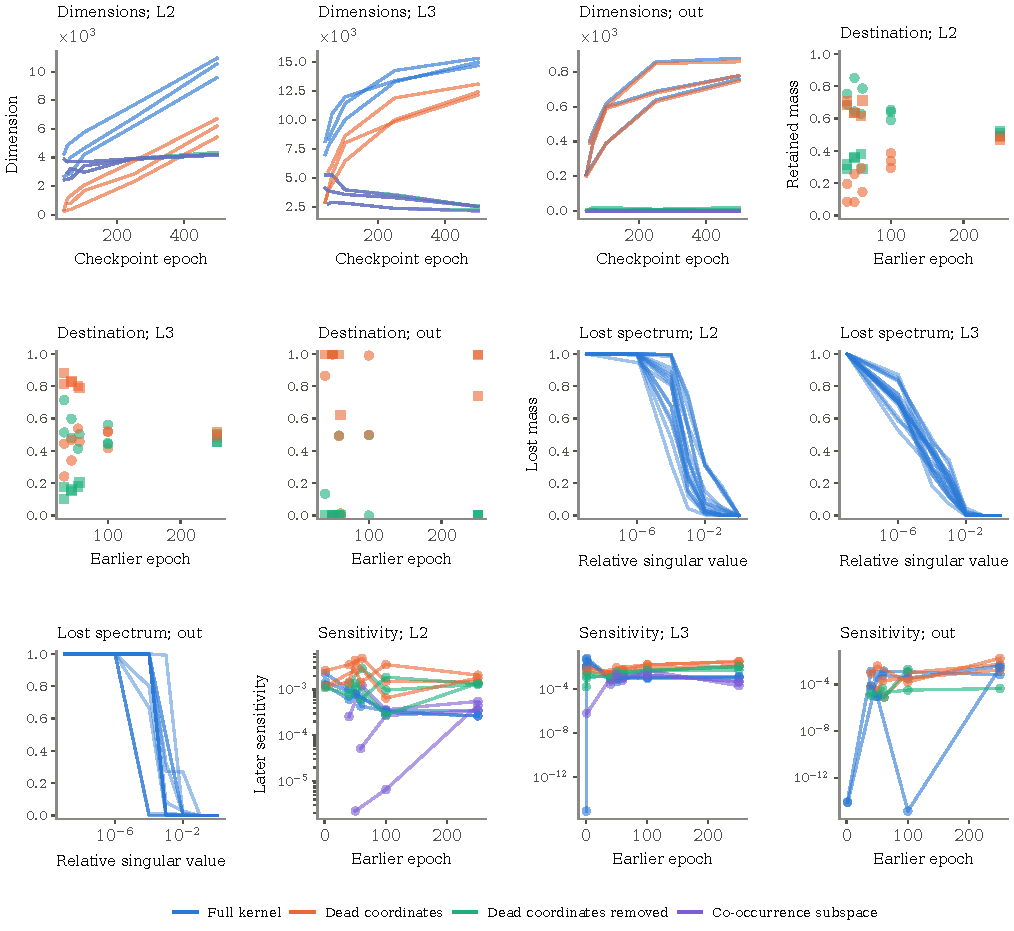
\includegraphics[width=6.081in]{persistence_diagnostics.pdf}
\caption{Further ReLU persistence diagnostics, all measured layers, pairs and three seeds. Panels 1--3: dimensions of the full kernel and its component spaces. Panels 4--6: the earlier kernel with dead coordinates removed, split into mass retained in later non-dead directions (green) and later dead coordinates (orange); circles denote consecutive pairs and squares comparisons ending at epoch 500. Panels 7--9: cumulative lost mass carried by later singular directions above each relative singular-value threshold. Panels 10--12: median later sensitivity of 32 sampled directions from the earlier kernel (blue) and its positive tails at thresholds $10^{-3}$ (orange), $10^{-4}$ (green) and $10^{-6}$ (purple). Missing curves denote empty or unresolved spaces.}\label{fig:persistence-diagnostics}
\end{figure}
\begin{table}[!htbp]\centering
\caption{GELU numerical dead-coordinate sensitivity at epoch 500, width 128. A unit is counted when its derivative magnitude is at most $\tau$ on every analysis image. Coordinate dimensions are seed ranges. The last columns count seeds whose dead-coordinate and co-occurrence projector splits resolve, out of three. The co-occurrence split remains unresolved at the endpoint.}\label{tab:persistence-gelu-tau}
\small\begin{tabular}{llrrr}\toprule
Layer & $\tau$ & Coordinate dimension & Dead split & Deficit split\\\midrule
2 & $10^{-9}$ & 258--774 & 3/3 & 0/3\\
3 & $10^{-9}$ & 256--768 & 3/3 & 0/3\\
2 & $10^{-6}$ & 774--1806 & 0/3 & 0/3\\
3 & $10^{-6}$ & 768--1792 & 1/3 & 0/3\\
2 & $10^{-3}$ & 2064--3096 & 0/3 & 0/3\\
3 & $10^{-3}$ & 2624--3282 & 0/3 & 0/3\\
\bottomrule\end{tabular}\end{table}\FloatBarrier


\FloatBarrier
\section{From function to loss, extended version}
\label{app:applications}
This section contains an extended discussion and additional preliminary observations regarding the topic of  Section~\ref{sec:discussion}: how functional invariance relates to loss invariance.

\subsection{Functional invariance and loss geometry}
\label{app:hessian}
The loss compresses a network's outputs to one scalar. A region with constant outputs therefore has constant data loss, but a constant loss can also arise while outputs move along a loss level set. We first make this distinction explicit for MSE, then measure how much of the numerical Hessian and GGN kernels is captured by the constructed compatible layerwise invariant subspaces.

\subsubsection{What functional invariance implies}
Let $Y=(y_i)_{i=1}^s$ be the target outputs, let $e=F_X(\theta_0)-Y$ be the residual at the base network, and use the data loss $\mathcal L(\theta)=\|F_X(\theta)-Y\|_X^2$. The associated inner product is $\langle U,V\rangle_X=s^{-1}\sum_i U_i^\top V_i$. For an edit $w$, expanding the square gives
\begin{equation}
 \mathcal L(\theta_0+w)-\mathcal L(\theta_0)
 =2\langle e,\Delta F_X(w)\rangle_X+\|\Delta F_X(w)\|_X^2.
 \label{eq:application-loss-change}
\end{equation}
Thus an exact ocean preserves the loss. If the outputs vary by at most $\varepsilon$, the absolute loss change is at most $2\|e\|_X\varepsilon+\varepsilon^2$. At exact interpolation, $e=0$, and the loss change is precisely the square of the functional change. This explains why visually flat loss landscapes can contain visible functional variation.

For differentiable loss and network maps, exact constancy of $\mathcal L(\theta_0+tv)$ near $t=0$ implies
\[
 0=\left.\frac{d}{dt}\mathcal L(\theta_0+tv)\right|_{t=0}
   =\nabla_\theta\mathcal L(\theta_0)^\top v
   =\nabla_F\mathcal L(F_X(\theta_0))^\top J_Xv.
\]
Functionally invisible directions satisfy this condition automatically. Other directions can move the outputs tangentially to a loss level set. For squared loss, the level set at value $c>0$ is $\{F:\|F-Y\|_X=\sqrt c\}$; a finite output trajectory on this sphere preserves loss while changing the function. At $c=0$ the level set reduces to $F=Y$. For softmax cross-entropy, let $\pi_i=\operatorname{softmax}(f_i)$ and write $u_i$ for a first-order logit change. Its first-order loss-preservation condition is $s^{-1}\sum_i(\pi_i-y_i)^\top u_i=0$, compared with $\langle e,u\rangle_X=0$ for MSE. When the respective output gradient is nonzero, each defines a hyperplane of dimension $sd-1$.  Adding $a_i\mathbf1$ to each sample's logit vector leaves its probabilities and cross-entropy unchanged at every amplitude. Such output transformations need not all be realizable by parameter edits. 

At a twice differentiable base point, write $H=\nabla^2\mathcal L(\theta_0)$ for the loss Hessian and $G=(2/s)J_X^\top J_X$ for its Gauss--Newton part. With $a$ indexing output coordinates,
\begin{equation}
 H=G+R,\qquad
 R=\frac{2}{s}\sum_{i=1}^s\sum_{a=1}^d e_{ia}\nabla^2 F_{ia}(\theta_0).
 \label{eq:application-hessian}
\end{equation}
Every exact ocean direction annihilates $J_X$ and hence $G$. It also belongs to $\ker H$ when $e=0$. With nonzero residual, constancy along a straight direction $v$ implies $v^\top Hv=0$, but can leave $Hv\ne0$: the Hessian may couple that direction to directions outside the ocean. For ReLU networks these statements apply in the interior of an activation chamber. The numerical comparisons below retain the signed Hessian spectrum and define near-nullity using absolute eigenvalues.

\subsubsection{Constructed-ocean coverage of numerical kernels}
We evaluate depth-3, width-64 ReLU MLPs trained on MNIST, at epoch 500, using three seeds and the fixed 10,000-example analysis set. Each network has $p=25{,}418$ parameters. The Hessian uses sample-averaged, output-summed MSE with one-hot targets and no regularization. The comparison space $M$ is the bottom-up layerwise invariant subspace after imposing compatibility, constructed independently of the curvature eigendecompositions and validated against the original-network Jacobian.

For $T\in\{H,G\}$, let $Q_{T,\tau}$ contain orthonormal eigenvectors with $|\lambda_T|\le\tau$, and let $d_{T,\tau}$ be their number. With an orthonormal basis $Q_M$ of the constructed space, define
\[
 C_T(\tau)=\frac{\|Q_M^\top Q_{T,\tau}\|_F^2}{d_{T,\tau}}.
\]
This is the mean squared projection of a target-band direction onto $M$. It measures average alignment, rather than intersection dimension or subspace inclusion. An isotropic random space of the same dimension has expected coverage $\dim M/p$.

At $\tau=10^{-14}$, Hessian coverage exceeds $1-10^{-8}$ in every seed, and GGN coverage is $94.34$--$96.21\%$ (Table~\ref{tab:kernel-coverage-dimensions}). These are numerical-kernel measurements: the saved float64 eigensolver has a noise floor of order $10^{-14}$, so classification at this scale cannot resolve exact algebraic zeros. At the looser cutoff $10^{-12}$, Hessian coverage remains $99.90$--$99.94\%$. We retain both signs of the Hessian spectrum when forming each band. The GGN is positive semidefinite up to roundoff.

\begin{table}[!htbp]\centering
\caption{Dimensions and coverage at numerical cutoff $10^{-14}$; $d_H,d_G$ count the numerical-kernel dimensions. The small Hessian projection deficits are retained for reproducibility and do not measure eigensolver accuracy. The isotropic random-space expectation is $\dim M/p$, with $p=25{,}418$.}
\label{tab:kernel-coverage-dimensions}
\small\begin{tabular}{crrrrrr}\toprule
Seed & $\dim M$ & $d_H$ & $d_G$ & Hessian (\%) & GGN (\%) & Random (\%)\\\midrule
0 & 3,619 & 3,200 & 3,836 & $100-9.5423\!\times\!10^{-10}$ & 94.34 & 14.2\\
1 & 4,573 & 4,116 & 4,753 & $100-2.2455\!\times\!10^{-10}$ & 96.21 & 18.0\\
2 & 4,072 & 3,434 & 4,281 & $100-2.7936\!\times\!10^{-9}$ & 95.06 & 16.0\\
\bottomrule\end{tabular}
\end{table}

\paragraph{Sensitivity to the target threshold.}
Figure~\ref{fig:fixed-ocean-coverage} increases the spectral threshold while retaining exactly the same constructed space at every threshold. The target bands grow to include small but nonzero curvature, and their coverage decreases. The right panel shows that growing denominator explicitly. These curves do not use approximate or enlarged oceans. The plotted mean and sample SD summarize the three seeds; they do not quantify uncertainty in numerical rank near the eigensolver floor.
\begin{figure}[!htbp]\centering
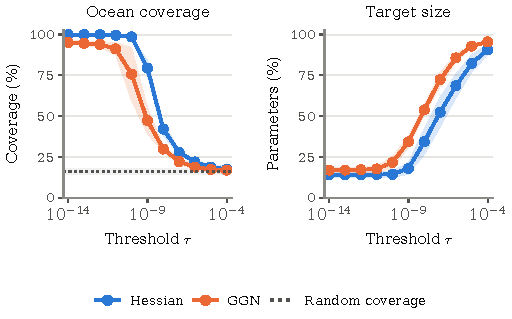
\includegraphics[width=3.074in]{fixed_ocean_coverage.pdf}
\caption{Coverage of Hessian and GGN bands $|\lambda|\le\tau$ by the fixed constructed layerwise invariant subspace (left), and target-band dimension as a percentage of all parameters (right). Lines and shading show mean $\pm$ sample SD across three seeds. The dotted reference is dimension-matched random coverage. Cutoffs near $10^{-14}$ approach numerical resolution.}
\label{fig:fixed-ocean-coverage}
\end{figure}


\subsubsection{Finite-distance behavior of curvature bands}
Figure~\ref{fig:curvature-cumulative-rays} tests the original network along random directions in the cumulative Hessian and GGN bands, using the protocol in Appendix~\ref{app:methods-curvature-rays}. The numerical kernels have visibility radii comparable to the constructed ocean. Enlarging a band changes both its dimension and its mixture of directions, so the finite-radius response need not vary monotonically with the eigenvalue cutoff. At output tolerance $10^{-3}$, the last safe tested radius of the median is 1 in every seed for the ocean, 1.5 for the Hessian band at $10^{-8}$, and 1 for the corresponding GGN band. At $10^{-4}$, these radii fall to 0.5 for the Hessian and 0.3--0.5 for the GGN, while generic directions reach only 0.003. These are sampled median responses, rather than uniform guarantees over either band.

\begin{figure}[!htbp]\centering
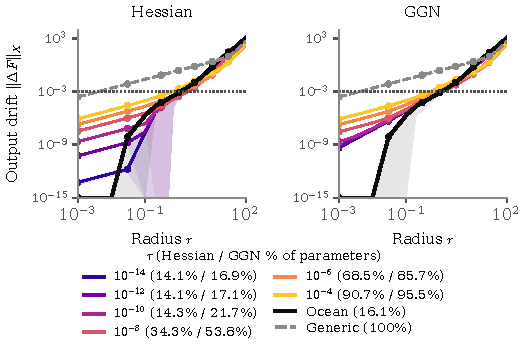
\includegraphics[width=3.165in]{curvature_cumulative_rays.pdf}
\caption{Cumulative Hessian and GGN bands $|\lambda_T|\le\tau$ in width-64 ReLU MNIST MLPs at epoch 500. Curves show mean $\pm$ sample SD of the three seed medians, each over 256 sampled directions. Legend percentages give mean dimensions relative to all parameters (Hessian / GGN). Black: constructed ocean; dashed gray: generic directions. The dotted line marks output drift $10^{-3}$.}\label{fig:curvature-cumulative-rays}
\end{figure}

\subsection{Linear mode connectivity}
\label{app:lmc}
Linear mode connectivity (LMC) asks whether the straight parameter segment between two trained networks maintains low loss. In this preliminary study, we examine whether shared ocean structure helps explain why networks descended from a common training checkpoint can remain functionally close.

\subsubsection{Loss and functional connectivity}
We study MNIST ReLU MLPs with three hidden layers of width 128 and the MNIST CNN. Each parent checkpoint is copied into two children, which inherit its parameters and Adam state and continue to epoch 500 with different minibatch orders. We compare these siblings with independently trained networks, using the protocol in Appendix~\ref{app:methods-lmc}.

For endpoint parameters $\theta_A,\theta_B$, let $\theta_\alpha=(1-\alpha)\theta_A+\alpha\theta_B$, with $\alpha\in[0,1]$, and let $F_A,F_B$ be their outputs on the evaluation set $X$. Loss connectivity concerns the largest loss excess along the segment above the chord joining its endpoint losses. To measure functional connectivity, we use the mean distance to the endpoint functions,
\[
 E(\alpha)=\tfrac12\bigl(\|F_X(\theta_\alpha)-F_A\|_X+
 \|F_X(\theta_\alpha)-F_B\|_X\bigr).
\]
Smaller values mean closer functions; even at an endpoint, this quantity includes half the difference between the endpoint functions. The additional chord-deviation measurement in Figure~\ref{fig:lmc-segments} measures departure from linear interpolation in output space, as defined in Appendix~\ref{app:methods-lmc}.

Most sibling pairs maintain low loss, while the independent-network segments have much larger barriers. Sibling functions also remain closer along their connection, especially after later forks. On the test set, stable loss and classification error coexist with more visible output variation. The parent--sibling planes in Figure~\ref{fig:lmc-landscape-full} illustrate the same distinction between a low-loss region and functional invariance.
\begin{figure}[!htbp]\centering
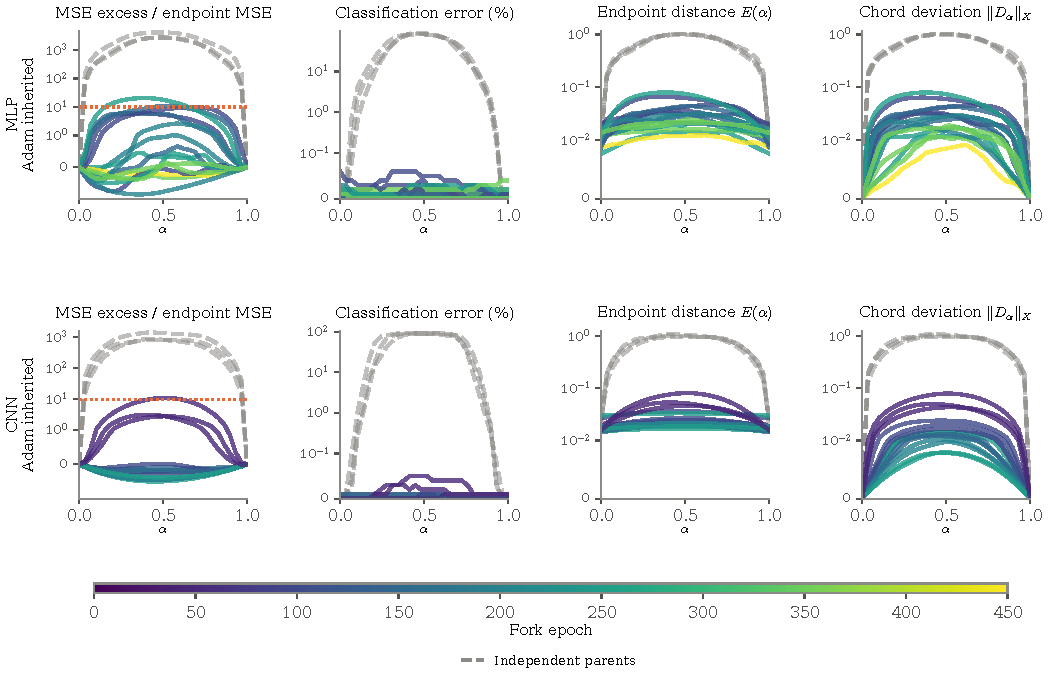
\includegraphics[width=6.291in]{lmc_segments_analysis.pdf}
\caption{Sibling connectivity on 10,000 training examples: MLPs above CNNs. Colors identify fork epochs for 16 MLP and 15 CNN sibling pairs; gray dashed curves show independently trained pairs. Columns show loss excess relative to the endpoint chord, normalized by mean endpoint loss; classification error; endpoint functional distance $E(\alpha)$; and output chord deviation. The dotted loss-connectivity threshold is 10.}\label{fig:lmc-segments}\label{fig:lmc-loss}
\end{figure}
\begin{figure}[!htbp]\centering
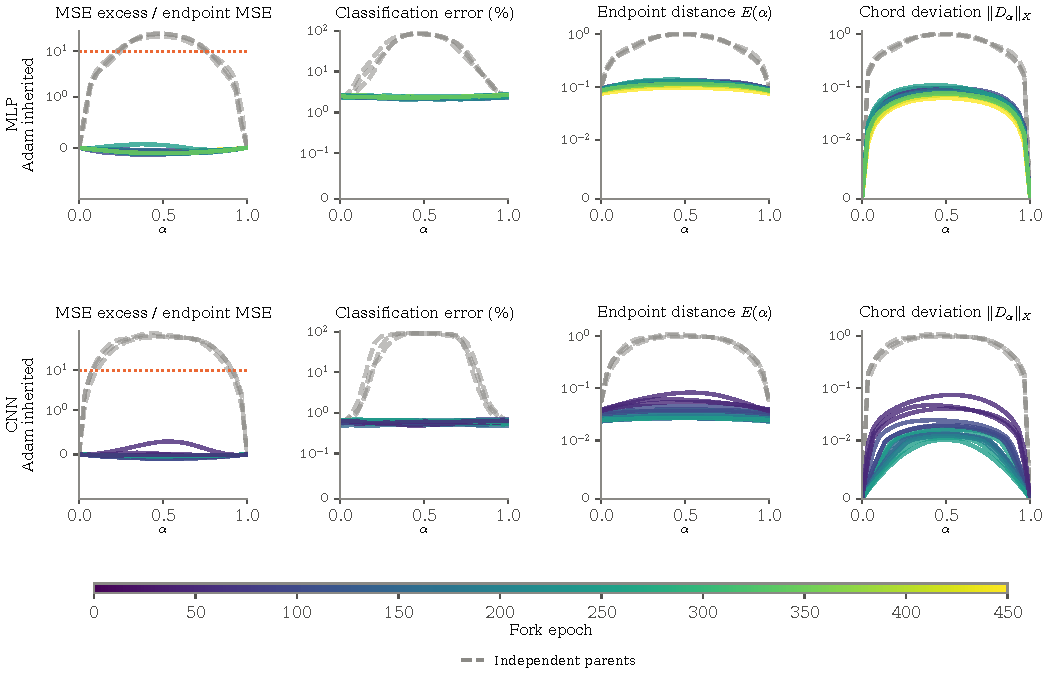
\includegraphics[width=6.291in]{lmc_segments_test.pdf}
\caption{The same connections on the separate 10,000-example test set, in the format of Figure~\ref{fig:lmc-segments}. Low loss and error can coexist with appreciable functional variation.}\label{fig:lmc-segments-test}
\end{figure}
\begin{figure}[!htbp]\centering
\begin{minipage}[t]{.49\linewidth}\centering
\textbf{MLP}\par\smallskip
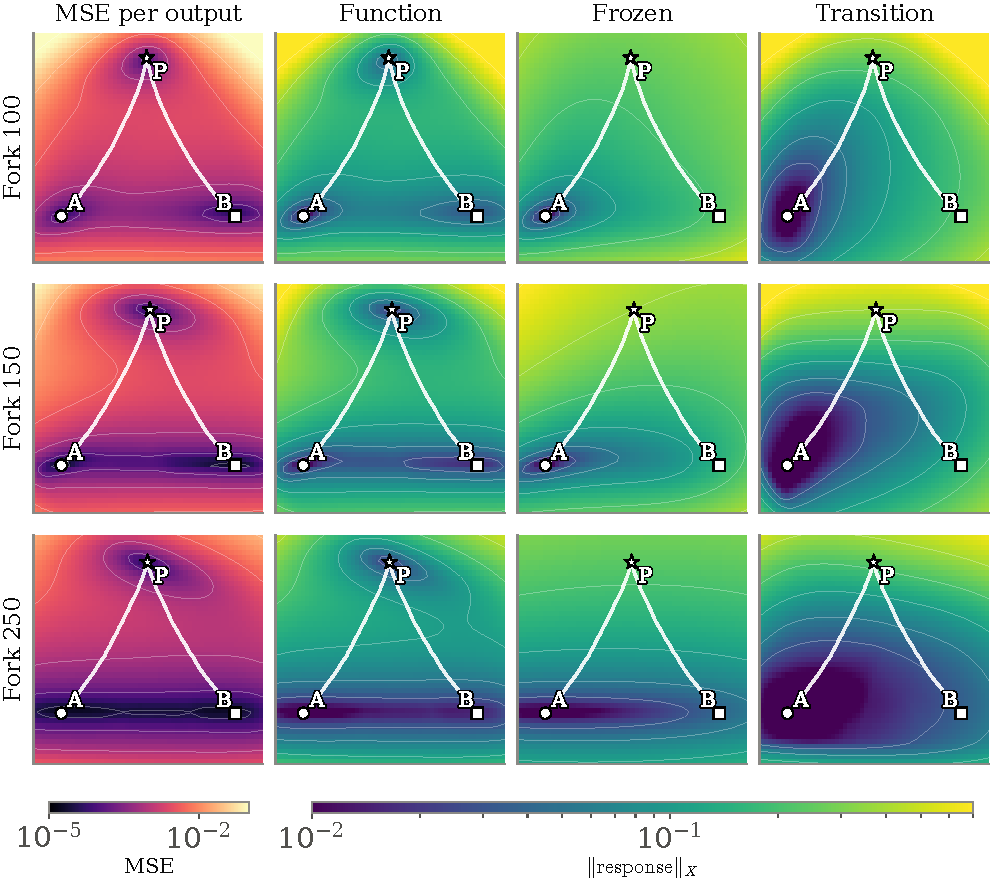
\includegraphics[width=\linewidth]{lmc_planes_mlp.pdf}
\end{minipage}\hfill
\begin{minipage}[t]{.49\linewidth}\centering
\textbf{CNN}\par\smallskip
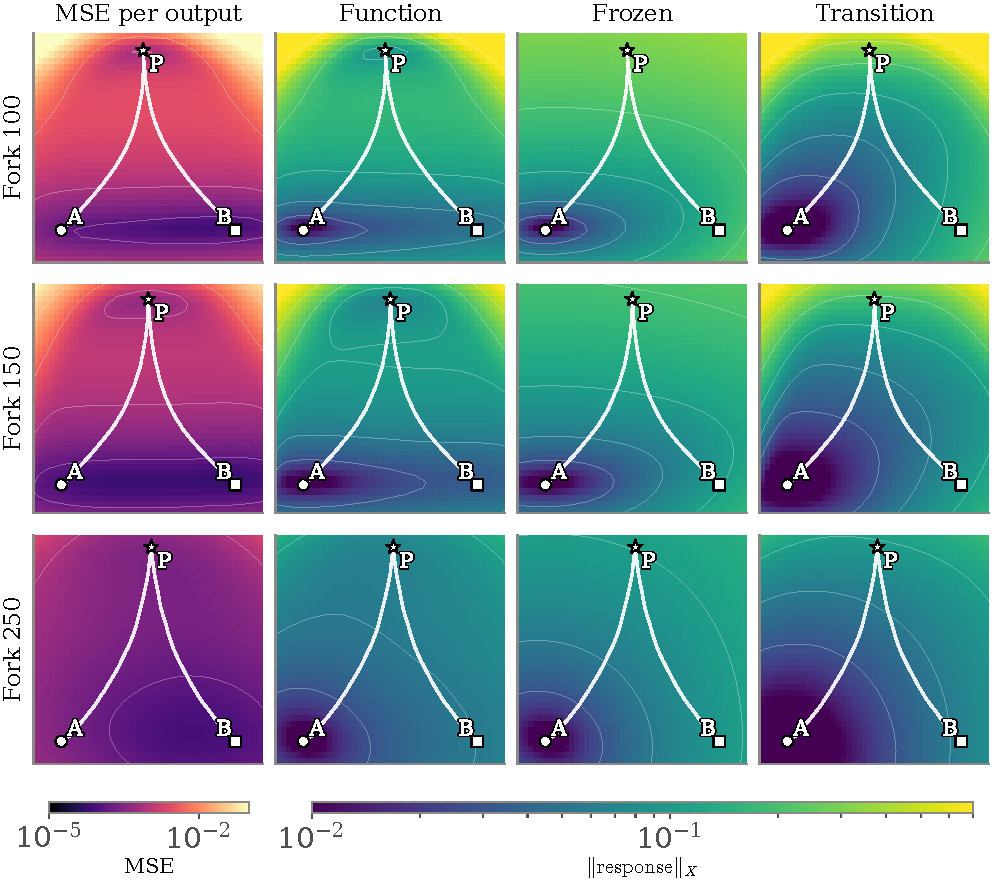
\includegraphics[width=\linewidth]{lmc_planes_cnn.pdf}
\end{minipage}
\caption{Planes through parent $P$ and sibling endpoints $A,B$, seed 0, with forks at epochs 100, 150 and 250 and endpoints at epoch 500. Columns show MSE per output, functional change from $A$, frozen response and activation transition. White curves are projected training trajectories. The MLP planes use 10,000 analysis examples; the CNN planes use 2,000. Functional norms and color scales match across architectures.}\label{fig:lmc-landscape-full}\label{fig:lmc-landscape-cnn}
\end{figure}

\FloatBarrier
\subsubsection{Parent--sibling ocean persistence}
\label{app:sibling-persistence}
The persistence results above suggest that siblings inherit substantial ocean structure. We ask whether they inherit \emph{the same} directions. We measure the intersections of parent and child atomic kernels in CNNs, using a principal-angle tolerance of $0.1^\circ$ and residual checks.

Table~\ref{tab:lmc-cnn-persistence} sums dimensions over all parameter layers and divides the sibling intersection by the mean of the two child dimensions. This shared fraction generally increases with later forks. The children also retain a substantial fraction of their parent's invariant directions, establishing common structure inherited through their separate training trajectories.
\begin{table}[!htbp]\centering\small
\caption{CNN parent--sibling persistence, mean $\pm$ sample SD across three seeds (percent). Dimensions are summed over all layers before normalization. Sibling sharing divides the child-intersection dimension by the mean child dimension; parent retention divides the parent--two-child intersection by the parent dimension. $n_P$ counts seeds with a nonempty parent space, used for retention.}\label{tab:lmc-cnn-persistence}
\begin{tabular}{rrrr}\toprule
Fork epoch & Sibling sharing & Parent retention & $n_P$\\\midrule
50 & $60.0\pm7.0$ & 100.0 & 1 \\
100 & $64.9\pm5.5$ & $88.6\pm11.8$ & 3 \\
150 & $73.0\pm4.6$ & $88.8\pm5.3$ & 3 \\
200 & $74.8\pm5.8$ & $82.1\pm2.6$ & 3 \\
250 & $74.9\pm8.4$ & $78.0\pm5.7$ & 3 \\\bottomrule\end{tabular}\end{table}


\subsubsection{Sharing of constructed endpoint subspaces}
\label{app:lmc-shared}
We compare the complete compatible layerwise invariant subspaces at sibling endpoints in three seeds per architecture: width-128 MLPs forked at epoch 350 and CNNs forked at epoch 200, with all children evaluated at epoch 500. The different fork times mean that this is not an architecture-only comparison. Let $Q_A,Q_B$ be orthonormal bases of the endpoint spaces, with dimensions $k_A,k_B$, and let $P_A=Q_AQ_A^\top$, $P_B=Q_BQ_B^\top$. Their continuous sharing fraction is
\[
 s_{AB}=\frac{\|Q_A^\top Q_B\|_F^2}{\min(k_A,k_B)}.
\]
This measures how much of the smaller space projects into the other, including partial alignments. No principal-angle filtering is applied. It is not the dimension of an intersection or a fraction of all parameters.

The endpoint spaces overlap strongly in both architectures (Table~\ref{tab:lmc-constructed-sharing}). This aggregate masks a layer-specific exception: MLP seed 1's L1 components have mean squared cosine $0.273$ and median principal angle $61.2^\circ$; L1 components are zero in the other two seeds. The remaining MLP components and the nonempty CNN late-layer components are more closely aligned.



\begin{table}[!htbp]\centering
\caption{Constructed sibling-space sharing and displacement projections, mean $\pm$ sample SD across three seeds. Projection entries are norm fractions; sequential projections measure continuous overlap.}
\label{tab:lmc-constructed-sharing}
\small\setlength{\tabcolsep}{4pt}
\begin{tabular}{lccccc}\toprule
Model & $100s_{AB}$ & $\|P_Ad\|/\|d\|$ & $\|P_Bd\|/\|d\|$ & $\|P_BP_Ad\|/\|d\|$ & $\|P_AP_Bd\|/\|d\|$\\\midrule
MLP & $93.9 \pm 6.4$ & $0.386 \pm 0.045$ & $0.382 \pm 0.046$ & $0.330 \pm 0.019$ & $0.330 \pm 0.019$\\
CNN & $85.0 \pm 6.0$ & $0.487 \pm 0.103$ & $0.503 \pm 0.106$ & $0.444 \pm 0.124$ & $0.445 \pm 0.123$\\\bottomrule\end{tabular}\end{table}





We also observe an intriguing pattern: siblings preserve a high fraction of activation gates along their connection, substantially more than independent networks (Figure~\ref{fig:lmc-gates}). Explaining how training produces this shared gate structure, and how it contributes to functional connectivity, is left to future work.
\begin{figure}[!htbp]\centering
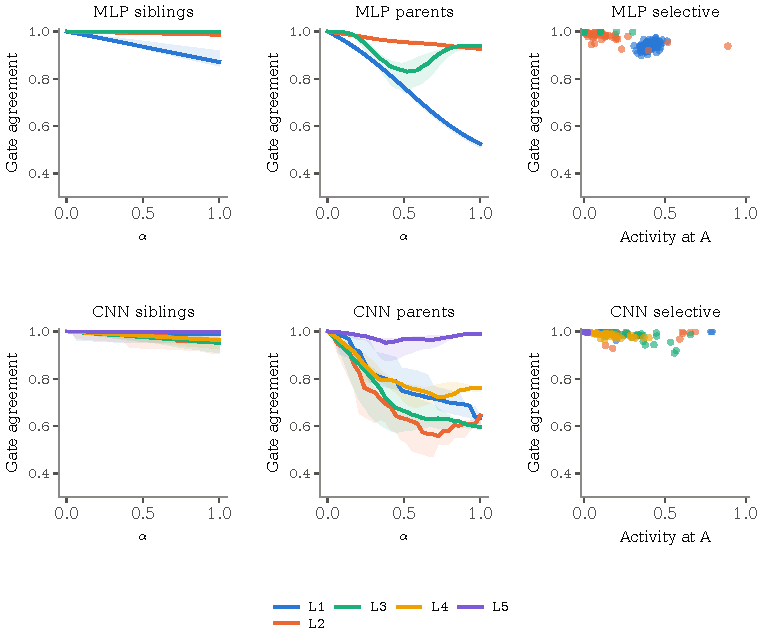
\includegraphics[width=4.585in]{lmc_gates_all.pdf}
\caption{Gate stability, MLP (first three panels) and CNN (last three). Sibling and independent-parent curves give median agreement with endpoint $A$ over all inherited-state pairs or independent pairs; bands span pairs. Selective-unit panels show activity at $A$ against midpoint gate agreement for seed 0, fork 250. Colors identify layers.}\label{fig:lmc-gates}\label{fig:lmc-selective}
\end{figure}
\FloatBarrier

\section{Additional material and plots}
\label{app:additional-material}
This section discusses the potential applications of Flat Oceans, sets out the open questions raised by the paper, then collects the ocean x-ray catalog and predictive-performance tables.

\subsection{Applications}
\label{app:finite-invariance-uses}

We give procedures to identify and construct a large region in which parameters can change while the network's outputs on an existing dataset remain controlled. Given reference parameters $\theta_0\in\mathbb R^p$, an orthonormal basis $Q\in\mathbb R^{p\times k}$ and a radius $r>0$ define such a region when
\begin{equation}
\mathcal O_{Q,r}=\{\theta_0+Qu:u\in\mathbb R^k,\ \|u\|_2\le r\},
\qquad
\sup_{\|u\|_2\le r}\|F_X(\theta_0+Qu)-F_X(\theta_0)\|_X\le\varepsilon.
\label{eq:operational-ocean}
\end{equation}
Both the dimension $k$ and the radius $r$ describe the available functional freedom. The applications below describe how this freedom could be used. We leave the development of algorithms in the specific areas to future work. 

\paragraph{Continual learning and adaptation.}
Several continual learning algorithms seek to optimize a new-task objective while preserving performance on old tasks. Orthogonal Gradient Descent \citep{farajtabar2020ogd} uses output-gradient constraints, and Elastic Weight Consolidation \citep{kirkpatrick2017ewc} uses Fisher-weighted penalties to discourage changes to important parameters. The flat ocean construction provides a finite region with explicit output-preservation control. Gradient Projection Memory's activation projections \citep{saha2021gpm} are closely related to our feature-null component. Our framework adds downstream and sample-pairing freedom and compatibility across layers, potentially enlarging the space available to fit new tasks.

\paragraph{Bayesian inference.}
Local Laplace approximations use curvature, often approximated by the GGN, to estimate posterior uncertainty \citep{daxberger2021laplace,immer2021linearization}. The flat directions are particularly consequential: weak likelihood curvature permits greater parameter uncertainty, yet small eigenvalues can be difficult to resolve accurately and are sensitive to numerical errors and curvature approximations. With an isotropic Gaussian prior of precision $\alpha>0$, a GGN eigenvalue $\lambda$ gives approximate posterior variance $(\lambda+\alpha)^{-1}$. Errors in small $\lambda$ can therefore substantially distort uncertainty when the prior precision is also small. Moreover, local curvature alone does not determine how far a flat direction extends. Flat oceans supply complementary information about finite regions over which the likelihood remains constant or controlled, potentially improving the quality of posterior approximations for neural network based models. 

\paragraph{Model editing and compression.}
Let $C:\mathbb R^p\to\mathbb R$ be an objective favoring a desired parameter property, such as smaller norms or sparsity. We can search for that property within the output-preserving region by solving
\begin{equation}
\min_{u\in\mathbb R^k,\ \|u\|_2\le r} C(\theta_0+Qu).
\label{eq:ocean-secondary-objective}
\end{equation}
Every feasible edit satisfies the output constraint in Equation~\ref{eq:operational-ocean}. For example, curvature-based pruning already exploits local loss information \citep{lecun1989brain}. The convexity of flat oceans makes it possible to run optimization programs over them.

\paragraph{Network analysis.}
The atomic decomposition identifies how features, downstream propagation and sample pairing create redundancy. The frozen/activation-remainder decomposition separates mixed-weight interactions from activation changes, providing a tool for studying finite updates even outside invariant regions.


\subsection{Open questions and future directions}
\label{app:future-work}
The present theory describes the invariant structure at a given network and dataset. Explaining how training produces this structure is the next central question. The observations also suggest applications and several extensions of the geometric theory.

\paragraph{Emergence, persistence and accretion.}
Training often enlarges the invariant subspaces while retaining many earlier directions (Appendix~\ref{app:persistence}). A dynamical account should explain how feature spans, downstream maps and their samplewise pairings evolve to create new atomic directions. It should also explain why existing directions survive later updates, so that growth can occur by accretion. Following the dimensions alone is insufficient: a theory must track the orientations of these spaces and the constraints that permit their composition.

\paragraph{Why the frozen approximation improves.}
The frozen network is defined at every checkpoint, but its accuracy over finite edits changes with training. The observed reduction of the activation remainder raises a question. Possible contributions include more stable ReLU gates, smaller local activation curvature for smooth networks, and weaker downstream propagation of activation residuals. Relating these mechanisms to learning extends existing analyses of gates and active paths \citep{lakshminarayanan2020paths}.

\paragraph{Training data and representation compression.}
In the matched comparisons of Appendix~\ref{app:training-data}, the full-data model has larger hidden atomic kernels than a model trained on a small subset, even when both are evaluated on that subset. Why can learning from more data produce more functional freedom? One question is whether additional data encourage compression of the feature and downstream spans, or change their pairings so that fewer independent output constraints remain. This concerns representations learned by different networks. For a fixed network, adding evaluation samples can only remove exact invariant directions. A dynamical explanation must account for both effects and the nonmonotone trends within the reduced-data training sweep.

\paragraph{Invariant subspace extent and unseen inputs.} The uniform norm bounds on the activation remainder can be much looser than measured radii. A sharper account should retain residual directions, downstream suppression and cancellations to characterize the extent of each invariant subspace at a prescribed tolerance. It must also connect sampled ray lengths to a guarantee over the whole invariant subspace ball. Extending finite-dataset certificates to unseen inputs requires controlling new feature and downstream constraints; the empirical transfers in Appendix~\ref{app:data-dependence} provide a starting point.

\paragraph{Maximum dimensions and efficient invariant subspace tests.}
Determining the maximum ocean dimension for nonlinear networks of arbitrary depth remains open, both for layerwise constructions and for general coupled invariant subspaces. Even the deep-linear subspace optimization requires a finite, efficient method for selecting target orientations. The general polynomial coefficient test is exact but becomes expensive with dimension and depth. Exploiting network structure to certify or construct large invariant subspaces without enumerating all coefficient constraints is an important algorithmic problem.

\paragraph{Flat symmetries across architectures.}
A systematic study should characterize flat symmetries in the full range of frozen network architectural structures. The convolutional and LayerNorm constructions here provide starting points for attention, residual connections, parameter sharing, normalization and other structured blocks. The aim is to identify which architectural identities create exact flat directions, which spaces arise from learned representations on a dataset, and when these directions compose across different block types.

\paragraph{Exceptional smooth cancellations.}
Appendix~\ref{app:smooth-exact} conjectures that, for tanh, sigmoid and softplus MLPs, the direction space of every exact local ocean is a frozen invariant subspace outside a Lebesgue-null set of data and base parameters. The one-unit calculation establishes only a special case. A general proof must exclude cancellations among units, paths and samples that persist at every order. The measure-zero claim concerns exceptional data and base parameters; the intrinsic volume of an ocean in its own affine hull is a different quantity. The reciprocal-affine counterexample shows why the activation assumptions matter.



\subsection{Ocean x-rays}
\label{app:xray}


The catalog collects the available two-dimensional parameter slices across ReLU and leaky-ReLU MLPs, GELU MLPs, CNNs, width and depth sweeps, and several direction constructions. Each Cartesian map shows the output response to two simultaneous parameter edits. Its angle--radius companion shows the same plane over a wider range of distances. The color scale is shared across the catalog, and each panel retains its own parameter scale.

White contours separate sampled points with unchanged gates from points with changed gates; black dashed contours mark output change $10^{-3}$. Their separation shows that gate changes can precede visible functional change. Smooth-activation panels have no ReLU chamber boundary. All views are measurements in selected planes; they do not certify the radius of an entire parameter subspace. The parent--sibling planes are reported separately in Appendix~\ref{app:lmc}.

\begin{figure}[!htbp]\centering
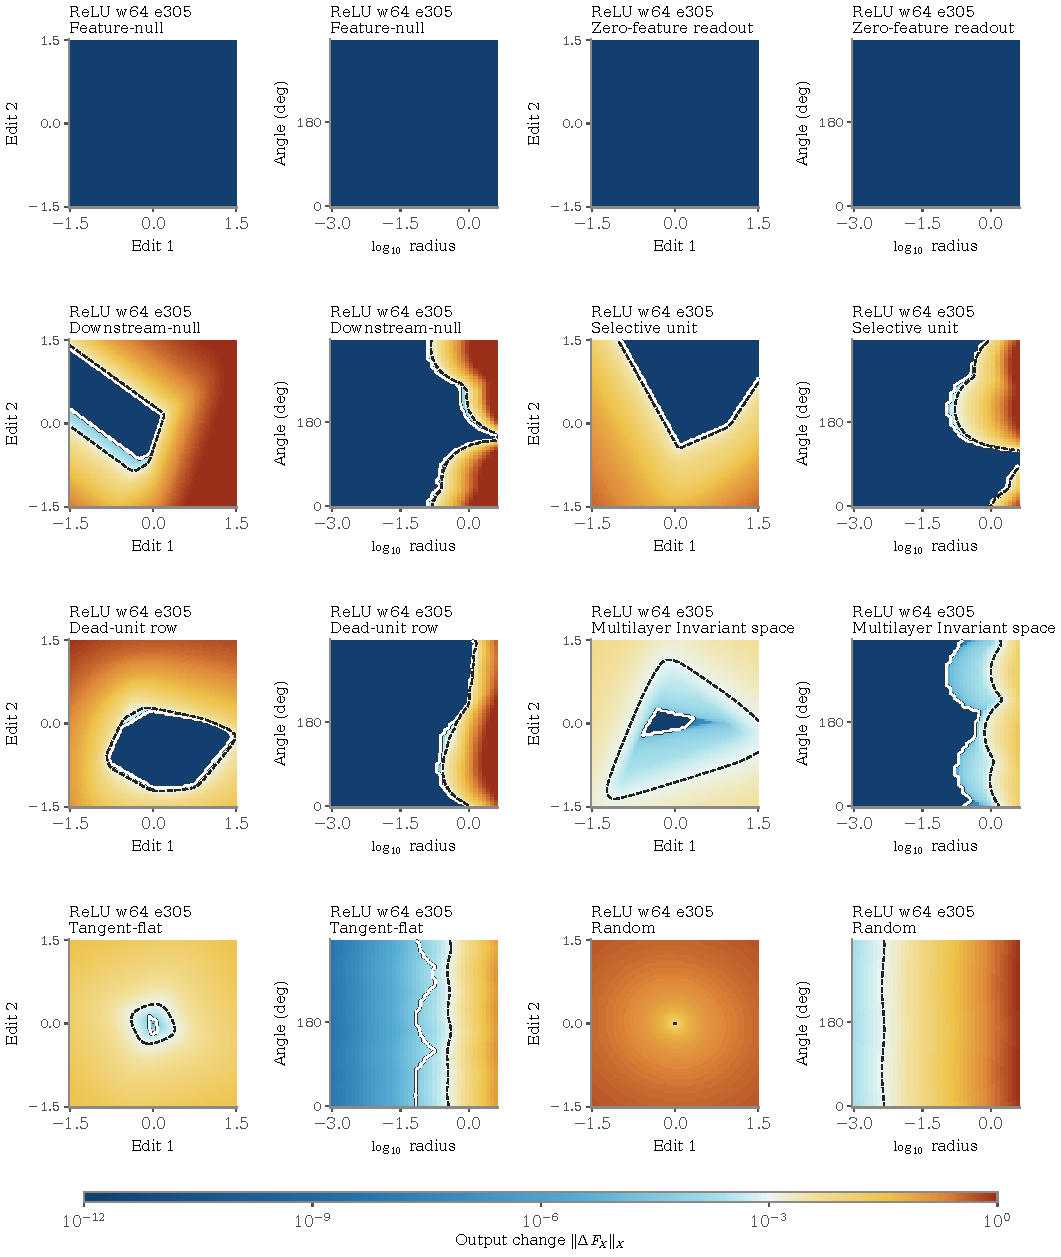
\includegraphics[width=6.367in]{xray_catalogue_1.pdf}
\caption{Ocean x-ray catalog, page 1. All panels use MNIST and seed 0; titles give width (w), hidden depth (d), and checkpoint epoch (e). Adjacent Cartesian and angle--radius panels describe the same two-dimensional parameter plane. The final seven angle--radius panels of the catalog compare selective directions in width and depth sweeps; width sweeps have depth three and depth sweeps have width 128. White contours separate the sampled zero-gate-change region from changed gates, and black dashed contours mark output change $10^{-3}$. All panels share the color scale; values below $10^{-12}$ use its lowest color. See the text for the scope of these sampled views.}\label{fig:xray-catalogue-1}
\end{figure}
\FloatBarrier\begin{figure}[!htbp]\centering
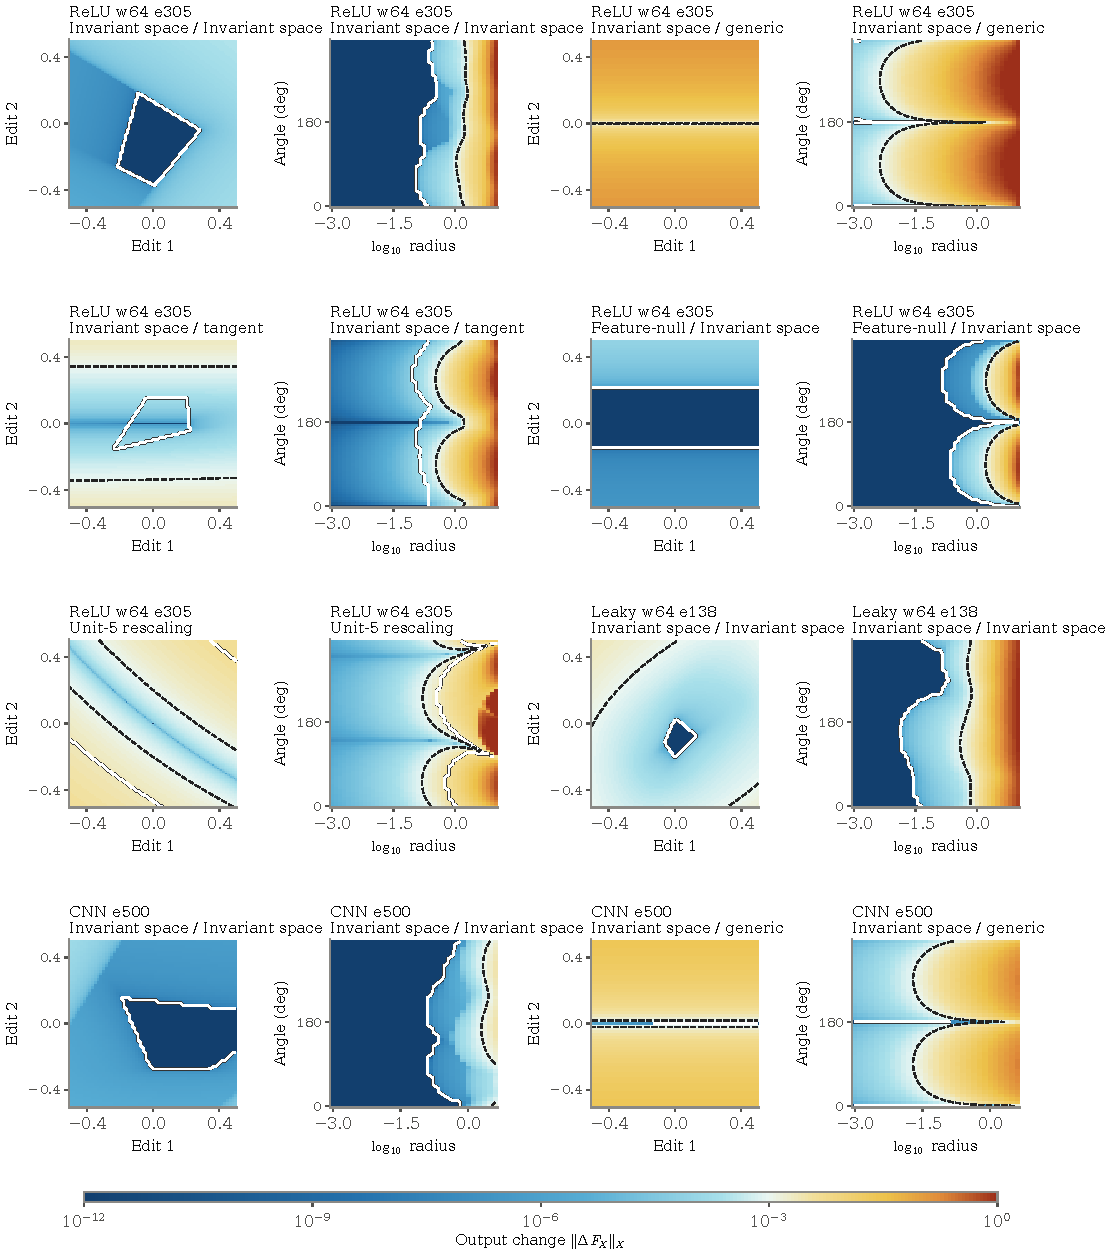
\includegraphics[width=6.662in]{xray_catalogue_2.pdf}
\caption{Ocean x-ray catalog, continued. Conventions and color scale as in Figure~\ref{fig:xray-catalogue-1}.}\label{fig:xray-catalogue-2}
\end{figure}
\FloatBarrier\begin{figure}[!htbp]\centering
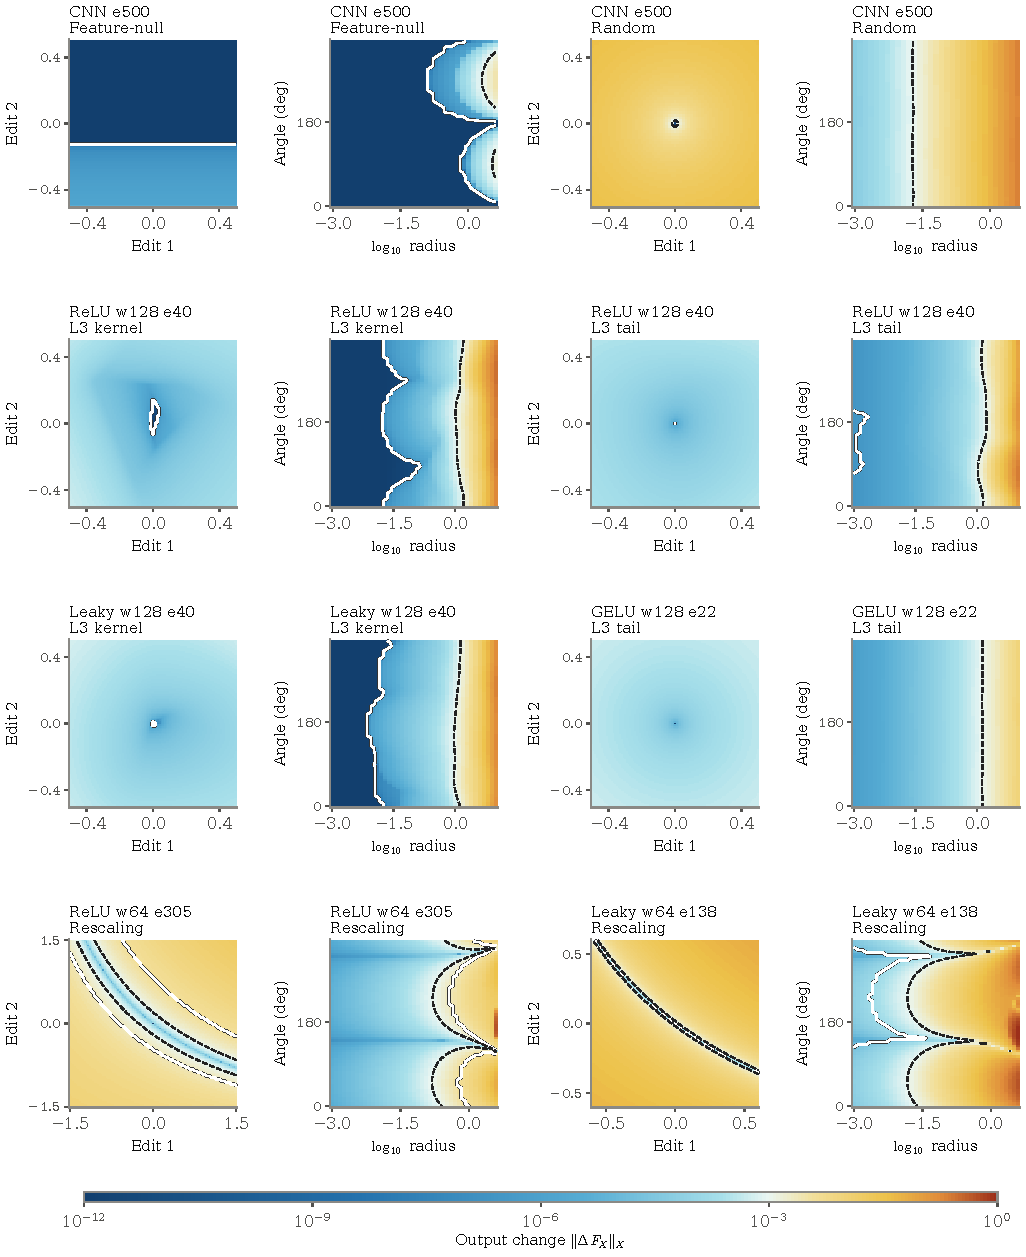
\includegraphics[width=6.156in]{xray_catalogue_3.pdf}
\caption{Ocean x-ray catalog, continued. Conventions and color scale as in Figure~\ref{fig:xray-catalogue-1}.}\label{fig:xray-catalogue-3}
\end{figure}
\FloatBarrier\begin{figure}[!htbp]\centering
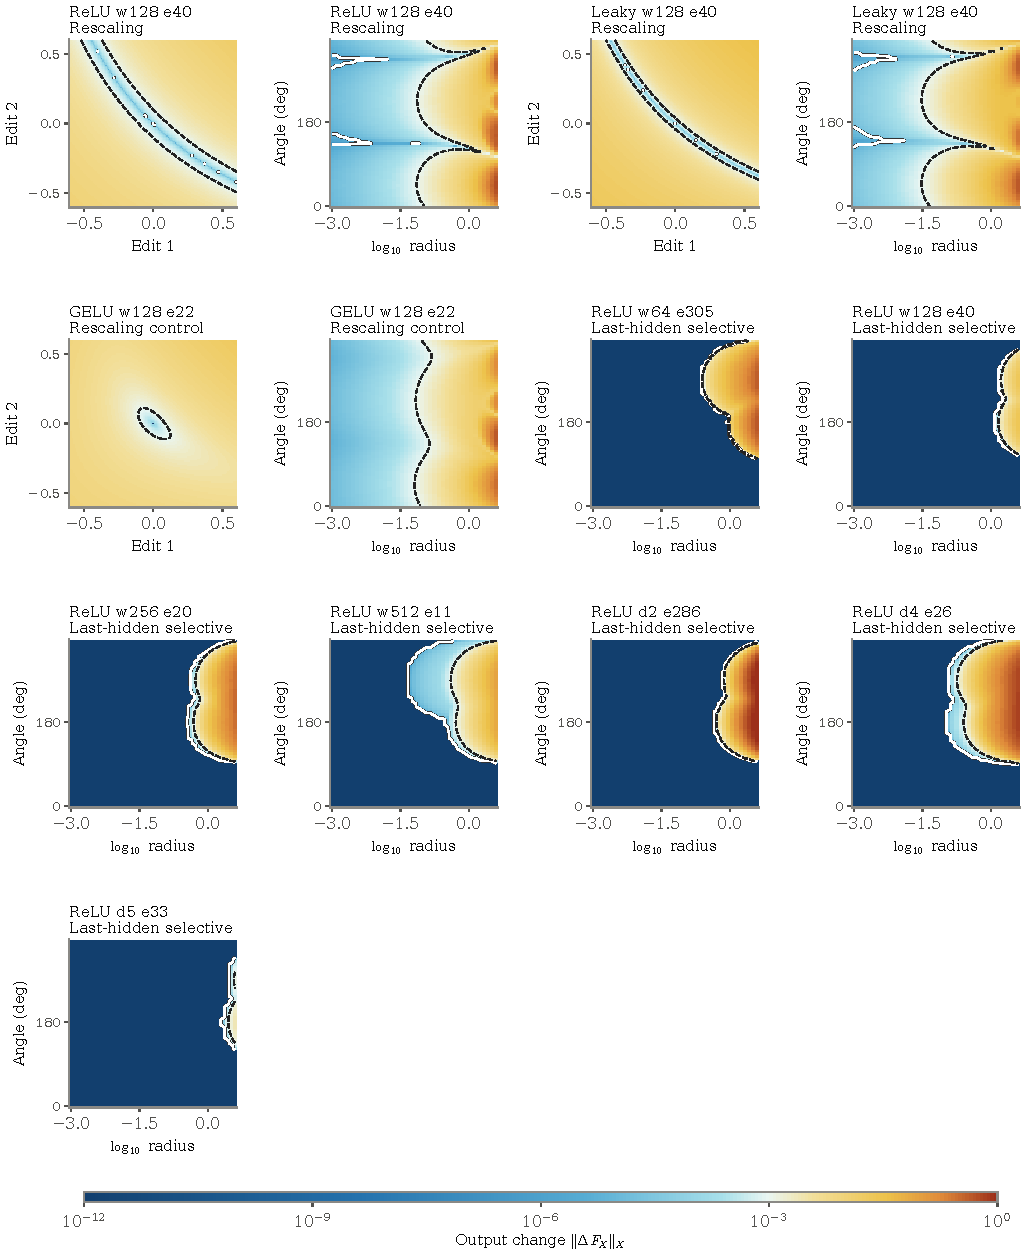
\includegraphics[width=6.156in]{xray_catalogue_4.pdf}
\caption{Ocean x-ray catalog, continued. Conventions and color scale as in Figure~\ref{fig:xray-catalogue-1}.}\label{fig:xray-catalogue-4}
\end{figure}
\FloatBarrier\FloatBarrier

\FloatBarrier

\subsection{Training and test performance}
\label{app:performance}
The tables report accuracy at declared analysis stages and the intermediate checkpoints used for descriptive comparisons. Values come from the saved training histories at the actual checkpoint epoch, rather than from the earlier epoch at which a milestone was first crossed. Ranges use only available seeds, whose count is shown. Unreached milestones are omitted; no endpoint substitutes for them. Width-128, depth-three ReLU is the reference for both scaling grids. The identity model's recorded matched comparisons retain their own checkpoint epochs.

The raw/PCA, normalization, activation and dataset comparisons use the same reporting convention. Reduced-data tables report accuracy on the fitted subset and the full test set. Margin-regularized models additionally report unregularized training MSE and parameter norms, since an apparent radius change can accompany a change in fitting or scale. ViT uses cross-entropy and records online augmented training accuracy, as stated in Table~\ref{tab:native-vit-training}.

\begin{table}[!htbp]\centering
\caption{Reference and activations: train and test accuracy at declared analysis stages and descriptive checkpoints. Entries are ranges across the available seeds; epochs may differ by seed. Unreached milestones have no row.}\label{tab:perf-0-0}
\small\setlength{\tabcolsep}{4pt}
\begin{tabular}{llrrrr}\toprule
Model & Stage & Epoch & Seeds & Train (\%) & Test (\%)\\\midrule
ReLU, width 128 & Init. & 0 & 3 & 6.082--9.805 & 6.150--9.860\\
 & Early fit & 1--2 & 3 & 90.433--93.617 & 90.200--93.000\\
 & High accuracy & 40--50 & 3 & 99.900--99.927 & 97.310--97.650\\
 & Interpolation & 50--61 & 3 & 99.945--99.953 & 97.350--97.620\\
 & Epoch 50 & 50 & 3 & 99.927--99.945 & 97.310--97.590\\
 & Epoch 100 & 100 & 3 & 99.963--99.982 & 97.440--97.480\\
 & Epoch 150 & 150 & 3 & 99.968--99.998 & 97.450--97.680\\
 & Epoch 200 & 200 & 3 & 99.957--99.990 & 97.440--97.530\\
 & Epoch 250 & 250 & 3 & 99.978--100.000 & 97.380--97.580\\
 & Endpoint & 500 & 3 & 99.987--99.998 & 97.300--97.640\\
\midrule
Leaky ReLU, width 128 & Init. & 0 & 3 & 6.420--10.210 & 6.390--10.150\\
 & Early fit & 1--2 & 3 & 90.972--93.843 & 90.800--93.050\\
 & High accuracy & 40--48 & 3 & 99.903--99.915 & 97.810--97.860\\
 & Interpolation & 66--81 & 3 & 99.962--99.968 & 97.820--97.870\\
 & Epoch 50 & 50 & 3 & 99.863--99.928 & 97.540--97.810\\
 & Epoch 100 & 100 & 3 & 99.860--99.977 & 97.560--97.760\\
 & Epoch 150 & 150 & 3 & 99.832--99.995 & 97.020--97.920\\
 & Epoch 200 & 200 & 3 & 99.988--100.000 & 97.780--97.850\\
 & Epoch 250 & 250 & 3 & 99.992--99.998 & 97.800--97.890\\
 & Endpoint & 500 & 3 & 99.998--100.000 & 97.730--97.860\\
\midrule
GELU, width 128 & Init. & 0 & 3 & 6.612--10.407 & 6.530--10.710\\
 & Early fit & 1 & 3 & 90.667--92.163 & 90.580--91.880\\
 & High accuracy & 20--23 & 3 & 99.902--99.920 & 97.670--97.930\\
 & Interpolation & 41--42 & 3 & 99.982--99.990 & 97.710--97.780\\
 & Epoch 50 & 50 & 3 & 99.993 & 97.680--97.920\\
 & Epoch 100 & 100 & 3 & 99.998--100.000 & 97.740--97.810\\
 & Epoch 150 & 150 & 3 & 100.000 & 97.660--97.730\\
 & Epoch 200 & 200 & 3 & 99.978--100.000 & 97.590--97.780\\
 & Epoch 250 & 250 & 3 & 100.000 & 97.490--97.820\\
 & Endpoint & 500 & 3 & 99.968--100.000 & 97.520--97.660\\
\bottomrule\end{tabular}\end{table}

\FloatBarrier
\begin{table}[!htbp]\centering
\caption{Reference and activations: train and test accuracy at declared analysis stages and descriptive checkpoints. Entries are ranges across the available seeds; epochs may differ by seed. Unreached milestones have no row. Identity checkpoints follow its recorded comparison; its own high-accuracy and interpolation milestones are not attained.}\label{tab:perf-0-3}
\small\setlength{\tabcolsep}{4pt}
\begin{tabular}{llrrrr}\toprule
Model & Stage & Epoch & Seeds & Train (\%) & Test (\%)\\\midrule
Identity, width 128 & Init. & 0 & 3 & 10.770--14.468 & 10.630--14.330\\
 & Epoch 50 & 50 & 3 & 85.227--85.492 & 85.940--86.030\\
 & Epoch 100 & 100 & 3 & 85.113--85.173 & 85.410--85.890\\
 & Epoch 150 & 150 & 3 & 85.128--85.202 & 85.730--85.920\\
 & Epoch 200 & 200 & 3 & 85.053--85.583 & 85.880--86.340\\
 & Epoch 250 & 250 & 3 & 85.270--85.312 & 85.880--85.990\\
 & Endpoint & 500 & 3 & 85.125--85.397 & 85.770--86.210\\
\midrule
Leaky ReLU, width 64 & Init. & 0 & 3 & 8.305--11.187 & 8.220--11.150\\
 & Early fit & 2 & 3 & 90.197--91.633 & 90.300--91.550\\
 & High accuracy & 138--285 & 3 & 99.900--99.902 & 97.100--97.390\\
 & Interpolation & 251--468 & 3 & 99.927--99.950 & 97.260--97.440\\
 & Epoch 50 & 50 & 3 & 99.668--99.740 & 97.130--97.300\\
 & Epoch 100 & 100 & 3 & 99.825--99.877 & 97.330--97.480\\
 & Epoch 150 & 150 & 3 & 99.803--99.900 & 97.120--97.490\\
 & Epoch 200 & 200 & 3 & 99.867--99.915 & 97.180--97.380\\
 & Epoch 250 & 250 & 3 & 99.880--99.932 & 97.170--97.410\\
 & Endpoint & 500 & 3 & 99.917--99.968 & 97.120--97.300\\
\bottomrule\end{tabular}\end{table}

\FloatBarrier
\begin{table}[!htbp]\centering
\caption{MLP scaling: train and test accuracy at declared analysis stages and descriptive checkpoints. Entries are ranges across the available seeds; epochs may differ by seed. Unreached milestones have no row.}\label{tab:perf-1-0}
\small\setlength{\tabcolsep}{4pt}
\begin{tabular}{llrrrr}\toprule
Model & Stage & Epoch & Seeds & Train (\%) & Test (\%)\\\midrule
Width 32 & Init. & 0 & 3 & 6.262--13.848 & 5.820--14.450\\
 & Early fit & 5 & 3 & 92.838--94.217 & 92.470--93.690\\
 & Epoch 50 & 50 & 3 & 99.027--99.187 & 95.780--96.060\\
 & Epoch 100 & 100 & 3 & 99.212--99.472 & 95.540--95.720\\
 & Epoch 150 & 150 & 3 & 99.348--99.513 & 95.310--95.770\\
 & Epoch 200 & 200 & 3 & 99.385--99.502 & 95.110--95.630\\
 & Epoch 250 & 250 & 3 & 99.382--99.612 & 95.000--95.730\\
 & Endpoint & 500 & 3 & 99.485--99.635 & 95.030--95.760\\
\midrule
Width 64 & Init. & 0 & 3 & 8.943--11.245 & 9.150--11.510\\
 & Early fit & 2 & 3 & 90.062--91.297 & 89.980--91.300\\
 & High accuracy & 188--313 & 3 & 99.900--99.910 & 96.710--96.910\\
 & Interpolation & 364 & 1 & 99.940 & 96.870\\
 & Epoch 50 & 50 & 3 & 99.687--99.725 & 96.610--97.050\\
 & Epoch 100 & 100 & 3 & 99.753--99.850 & 96.890--96.970\\
 & Epoch 150 & 150 & 3 & 99.688--99.873 & 96.760--96.880\\
 & Epoch 200 & 200 & 3 & 99.857--99.907 & 96.900--97.190\\
 & Epoch 250 & 250 & 3 & 99.822--99.890 & 96.770--97.000\\
 & Endpoint & 500 & 3 & 99.897--99.960 & 96.740--96.870\\
\midrule
Width 256 & Init. & 0 & 3 & 9.365--11.188 & 9.840--11.590\\
 & Early fit & 1 & 3 & 93.267--93.405 & 92.750--92.890\\
 & High accuracy & 16--25 & 3 & 99.902--99.933 & 97.870--97.940\\
 & Interpolation & 31--47 & 3 & 99.978--99.982 & 97.900--98.100\\
 & Epoch 50 & 50 & 3 & 99.982--99.987 & 97.920--98.060\\
 & Epoch 100 & 100 & 3 & 99.973--99.992 & 97.750--98.020\\
 & Epoch 150 & 150 & 3 & 99.975--99.992 & 97.760--97.950\\
 & Epoch 200 & 200 & 3 & 99.987--100.000 & 97.870--98.060\\
 & Epoch 250 & 250 & 3 & 99.995--99.997 & 97.700--98.170\\
 & Endpoint & 500 & 3 & 99.978--99.992 & 97.560--97.790\\
\bottomrule\end{tabular}\end{table}

\FloatBarrier
\begin{table}[!htbp]\centering
\caption{MLP scaling: train and test accuracy at declared analysis stages and descriptive checkpoints. Entries are ranges across the available seeds; epochs may differ by seed. Unreached milestones have no row.}\label{tab:perf-1-3}
\small\setlength{\tabcolsep}{4pt}
\begin{tabular}{llrrrr}\toprule
Model & Stage & Epoch & Seeds & Train (\%) & Test (\%)\\\midrule
Width 512 & Init. & 0 & 3 & 7.437--9.718 & 7.080--9.690\\
 & Early fit & 1 & 3 & 95.055--95.240 & 94.190--94.590\\
 & High accuracy & 10--11 & 3 & 99.902--99.928 & 97.900--98.080\\
 & Interpolation & 34--36 & 3 & 99.988--99.998 & 98.120--98.360\\
 & Epoch 50 & 50 & 3 & 99.995 & 98.140--98.280\\
 & Epoch 100 & 100 & 3 & 99.977--99.998 & 98.000--98.240\\
 & Epoch 150 & 150 & 3 & 99.993--99.997 & 97.890--98.050\\
 & Epoch 200 & 200 & 3 & 99.985--99.998 & 97.860--98.030\\
 & Epoch 250 & 250 & 3 & 99.957--100.000 & 97.820--97.930\\
 & Endpoint & 500 & 3 & 99.993--99.997 & 97.640--97.710\\
\midrule
Depth 2 & Init. & 0 & 3 & 9.343--15.093 & 9.770--14.800\\
 & Early fit & 1--2 & 3 & 90.627--93.575 & 90.070--93.070\\
 & High accuracy & 85--286 & 3 & 99.900--99.910 & 96.620--97.230\\
 & Epoch 50 & 50 & 3 & 99.790--99.858 & 97.410--97.530\\
 & Epoch 100 & 100 & 3 & 99.855--99.917 & 97.100--97.180\\
 & Epoch 150 & 150 & 3 & 99.863--99.923 & 96.910--96.990\\
 & Epoch 200 & 200 & 3 & 99.877--99.920 & 96.690--96.820\\
 & Epoch 250 & 250 & 3 & 99.878--99.925 & 96.530--96.800\\
 & Endpoint & 500 & 3 & 99.900--99.928 & 96.260--96.810\\
\midrule
Depth 4 & Init. & 0 & 3 & 9.162--11.103 & 9.240--11.960\\
 & Early fit & 1 & 3 & 90.617--91.978 & 90.630--91.610\\
 & High accuracy & 26--28 & 3 & 99.900--99.913 & 97.390--97.720\\
 & Interpolation & 36--55 & 3 & 99.947--99.977 & 97.510--97.650\\
 & Epoch 50 & 50 & 3 & 99.923--99.972 & 97.420--97.800\\
 & Epoch 100 & 100 & 3 & 99.382--99.975 & 96.560--97.770\\
 & Epoch 150 & 150 & 3 & 99.992--99.997 & 97.510--97.860\\
 & Epoch 200 & 200 & 3 & 99.982--99.992 & 97.380--97.940\\
 & Epoch 250 & 250 & 3 & 99.995--99.997 & 97.720--97.790\\
 & Endpoint & 500 & 3 & 99.973--99.997 & 97.450--97.630\\
\bottomrule\end{tabular}\end{table}

\FloatBarrier
\begin{table}[!htbp]\centering
\caption{MLP scaling: train and test accuracy at declared analysis stages and descriptive checkpoints. Entries are ranges across the available seeds; epochs may differ by seed. Unreached milestones have no row.}\label{tab:perf-1-6}
\small\setlength{\tabcolsep}{4pt}
\begin{tabular}{llrrrr}\toprule
Model & Stage & Epoch & Seeds & Train (\%) & Test (\%)\\\midrule
Depth 5 & Init. & 0 & 3 & 8.527--11.118 & 8.810--11.410\\
 & Early fit & 1 & 3 & 91.198--91.833 & 90.710--91.630\\
 & High accuracy & 33--40 & 3 & 99.902--99.908 & 97.220--97.470\\
 & Interpolation & 48--82 & 3 & 99.962--99.977 & 97.370--97.550\\
 & Epoch 50 & 50 & 3 & 99.837--99.932 & 97.350--97.520\\
 & Epoch 100 & 100 & 3 & 99.950--99.982 & 97.610--97.710\\
 & Epoch 150 & 150 & 3 & 99.942--99.993 & 97.560--97.770\\
 & Epoch 200 & 200 & 3 & 99.865--99.993 & 97.570--97.680\\
 & Epoch 250 & 250 & 3 & 99.818--99.978 & 97.400--97.600\\
 & Endpoint & 500 & 3 & 99.992--99.993 & 97.740--97.810\\
\bottomrule\end{tabular}\end{table}

\FloatBarrier
\begin{table}[!htbp]\centering
\caption{Convolution and normalization: train and test accuracy at declared analysis stages and descriptive checkpoints. Entries are ranges across the available seeds; epochs may differ by seed. Unreached milestones have no row.}\label{tab:perf-2-0}
\small\setlength{\tabcolsep}{4pt}
\begin{tabular}{llrrrr}\toprule
Model & Stage & Epoch & Seeds & Train (\%) & Test (\%)\\\midrule
MNIST CNN, base & Init. & 0 & 3 & 9.068--9.890 & 8.970--9.640\\
 & Early fit & 1 & 3 & 96.607--96.872 & 96.940--97.030\\
 & High accuracy & 65--68 & 3 & 99.902--99.905 & 99.450--99.560\\
 & Interpolation & 281--385 & 3 & 99.998--100.000 & 99.360--99.480\\
 & Epoch 50 & 50 & 3 & 99.792--99.815 & 99.430--99.530\\
 & Epoch 100 & 100 & 3 & 99.962--99.977 & 99.450--99.540\\
 & Epoch 150 & 150 & 3 & 99.990--99.995 & 99.420--99.460\\
 & Epoch 200 & 200 & 3 & 99.997--99.998 & 99.420--99.520\\
 & Epoch 250 & 250 & 3 & 99.988--100.000 & 99.450--99.530\\
 & Endpoint & 500 & 3 & 99.998--100.000 & 99.370--99.490\\
\midrule
MNIST CNN, $0.5\times$ & Init. & 0 & 3 & 8.618--11.785 & 8.480--10.640\\
 & Early fit & 1 & 3 & 94.940--96.513 & 95.300--96.730\\
 & High accuracy & 384--446 & 3 & 99.900 & 99.000--99.360\\
 & Epoch 50 & 50 & 3 & 99.292--99.435 & 99.210--99.250\\
 & Epoch 100 & 100 & 3 & 99.565--99.603 & 99.300--99.420\\
 & Epoch 150 & 150 & 3 & 99.663--99.717 & 99.280--99.410\\
 & Epoch 200 & 200 & 3 & 99.715--99.788 & 99.300--99.410\\
 & Epoch 250 & 250 & 3 & 99.758--99.808 & 99.260--99.440\\
 & Endpoint & 500 & 3 & 99.903--99.923 & 99.030--99.200\\
\midrule
MNIST CNN, $2\times$ & Init. & 0 & 3 & 8.827--9.973 & 7.900--9.910\\
 & Early fit & 1 & 3 & 97.388--97.697 & 97.620--97.970\\
 & High accuracy & 31--35 & 3 & 99.903--99.917 & 99.480--99.580\\
 & Interpolation & 106--130 & 3 & 100.000 & 99.470--99.570\\
 & Epoch 50 & 50 & 3 & 99.980--99.985 & 99.510--99.590\\
 & Epoch 100 & 100 & 3 & 99.998--100.000 & 99.500--99.590\\
 & Epoch 150 & 150 & 3 & 100.000 & 99.440--99.610\\
 & Epoch 200 & 200 & 3 & 100.000 & 99.450--99.570\\
 & Epoch 250 & 250 & 3 & 100.000 & 99.490--99.570\\
 & Endpoint & 500 & 3 & 100.000 & 99.450--99.490\\
\bottomrule\end{tabular}\end{table}

\FloatBarrier
\begin{table}[!htbp]\centering
\caption{Convolution and normalization: train and test accuracy at declared analysis stages and descriptive checkpoints. Entries are ranges across the available seeds; epochs may differ by seed. Unreached milestones have no row.}\label{tab:perf-2-3}
\small\setlength{\tabcolsep}{4pt}
\begin{tabular}{llrrrr}\toprule
Model & Stage & Epoch & Seeds & Train (\%) & Test (\%)\\\midrule
BatchNorm, width 64 & Init. & 0 & 3 & 10.462--10.750 & 11.000--11.220\\
 & Early fit & 2 & 3 & 91.823--92.240 & 92.000--92.260\\
 & High accuracy & 51--56 & 3 & 99.905--99.910 & 97.300--97.620\\
 & Interpolation & 177--199 & 3 & 99.970--99.988 & 97.290--97.430\\
 & Epoch 50 & 50 & 3 & 99.873--99.897 & 97.290--97.660\\
 & Epoch 100 & 100 & 3 & 99.948--99.973 & 97.280--97.500\\
 & Epoch 150 & 150 & 3 & 99.967--99.983 & 97.440--97.490\\
 & Epoch 200 & 200 & 3 & 99.973--99.987 & 97.370--97.530\\
 & Epoch 250 & 250 & 3 & 99.982--99.985 & 97.290--97.440\\
 & Endpoint & 500 & 3 & 99.993--99.997 & 97.480--97.510\\
\bottomrule\end{tabular}\end{table}

\FloatBarrier
\begin{table}[!htbp]\centering
\caption{Input and dataset comparisons: train and test accuracy at declared analysis stages and descriptive checkpoints. Entries are ranges across the available seeds; epochs may differ by seed. Unreached milestones have no row.}\label{tab:perf-3-0}
\small\setlength{\tabcolsep}{4pt}
\begin{tabular}{llrrrr}\toprule
Model & Stage & Epoch & Seeds & Train (\%) & Test (\%)\\\midrule
Raw MNIST, width 64 & Init. & 0 & 3 & 10.075--13.660 & 10.130--13.130\\
 & Early fit & 1--2 & 3 & 91.455--93.277 & 91.730--92.930\\
 & High accuracy & 90--125 & 3 & 99.900--99.912 & 97.180--97.390\\
 & Interpolation & 224--379 & 3 & 99.952--99.955 & 97.270--97.360\\
 & Epoch 50 & 50 & 3 & 99.752--99.775 & 97.120--97.360\\
 & Epoch 100 & 100 & 3 & 99.833--99.877 & 97.130--97.190\\
 & Epoch 150 & 150 & 3 & 99.838--99.912 & 97.160--97.350\\
 & Epoch 200 & 200 & 3 & 99.882--99.948 & 97.190--97.370\\
 & Epoch 250 & 250 & 3 & 99.922--99.945 & 97.130--97.380\\
 & Endpoint & 500 & 3 & 99.957--99.975 & 97.020--97.460\\
\midrule
SVHN MLP, baseline & Init. & 0 & 3 & 9.044--10.077 & 8.812--9.496\\
 & Early fit & 40 & 3 & 90.026--90.555 & 80.059--80.374\\
 & Epoch 50 & 50 & 3 & 90.830--91.524 & 79.955--80.186\\
 & Epoch 100 & 100 & 3 & 92.585--93.177 & 79.168--79.940\\
 & Epoch 150 & 150 & 3 & 93.169--93.819 & 78.688--79.402\\
 & Epoch 200 & 200 & 3 & 93.295--94.103 & 78.350--79.007\\
 & Epoch 250 & 250 & 3 & 93.700--94.181 & 78.196--78.669\\
 & Endpoint & 500 & 3 & 94.080--94.788 & 77.704--77.812\\
\midrule
SVHN MLP, revised & Init. & 0 & 3 & 9.325--10.249 & 9.342--9.715\\
 & Early fit & 40--50 & 3 & 90.429--90.468 & 83.559--83.924\\
 & Epoch 50 & 50 & 3 & 90.429--90.630 & 83.559--84.139\\
 & Epoch 100 & 100 & 3 & 91.352--91.465 & 83.805--84.684\\
 & Epoch 150 & 150 & 3 & 91.670--91.793 & 83.897--84.542\\
 & Epoch 200 & 200 & 3 & 91.586--92.054 & 84.519--84.842\\
 & Epoch 250 & 250 & 3 & 91.819--91.917 & 84.404--84.753\\
 & Endpoint & 500 & 3 & 91.963--92.351 & 84.588--84.669\\
 & Validation selected & 371--494 & 3 & 91.960--92.235 & 84.315--84.577\\
\bottomrule\end{tabular}\end{table}

\FloatBarrier
\begin{table}[!htbp]\centering
\caption{Input and dataset comparisons: train and test accuracy at declared analysis stages and descriptive checkpoints. Entries are ranges across the available seeds; epochs may differ by seed. Unreached milestones have no row.}\label{tab:perf-3-3}
\small\setlength{\tabcolsep}{4pt}
\begin{tabular}{llrrrr}\toprule
Model & Stage & Epoch & Seeds & Train (\%) & Test (\%)\\\midrule
SVHN CNN & Init. & 0 & 3 & 7.707--13.379 & 8.032--12.957\\
 & Early fit & 5 & 3 & 91.178--92.904 & 90.124--91.841\\
 & High accuracy & 113--116 & 3 & 99.903--99.906 & 92.594--92.720\\
 & Epoch 50 & 50 & 3 & 99.244--99.428 & 94.000--94.111\\
 & Epoch 100 & 100 & 3 & 99.835--99.868 & 92.744--93.009\\
 & Epoch 150 & 150 & 3 & 99.947--99.951 & 92.286--92.482\\
 & Epoch 200 & 200 & 3 & 99.969--99.974 & 92.029--92.133\\
 & Epoch 250 & 250 & 3 & 99.977--99.978 & 91.683--91.829\\
 & Endpoint & 500 & 3 & 99.984--99.988 & 91.268--91.299\\
\bottomrule\end{tabular}\end{table}

\FloatBarrier
\begin{table}[!htbp]\centering
\caption{Reduced training samples: train and test accuracy at declared analysis stages and descriptive checkpoints. Entries are ranges across the available seeds; epochs may differ by seed. Unreached milestones have no row.}\label{tab:perf-4-0}
\small\setlength{\tabcolsep}{4pt}
\begin{tabular}{llrrrr}\toprule
Model & Stage & Epoch & Seeds & Train (\%) & Test (\%)\\\midrule
MNIST, $N=1{,}000$ & Init. & 0 & 3 & 6.600--11.200 & 6.150--9.860\\
 & Early fit & 20 & 3 & 94.000--97.600 & 64.610--70.220\\
 & High accuracy & 31--39 & 3 & 99.900 & 71.400--75.310\\
 & Interpolation & 184--209 & 3 & 100.000 & 74.060--77.210\\
 & Epoch 50 & 50 & 3 & 100.000 & 72.580--76.610\\
 & Epoch 100 & 100 & 3 & 100.000 & 74.130--77.340\\
 & Epoch 150 & 150 & 3 & 100.000 & 74.170--77.230\\
 & Epoch 200 & 200 & 3 & 100.000 & 74.070--77.150\\
 & Epoch 250 & 250 & 3 & 100.000 & 73.920--77.170\\
 & Endpoint & 500 & 3 & 100.000 & 73.790--77.040\\
\midrule
MNIST, $N=2{,}000$ & Init. & 0 & 3 & 6.350--10.750 & 6.150--9.860\\
 & Early fit & 20 & 3 & 97.550--98.650 & 77.090--81.450\\
 & High accuracy & 29--39 & 3 & 99.900 & 81.210--84.570\\
 & Interpolation & 212--238 & 3 & 100.000 & 82.230--83.920\\
 & Epoch 50 & 50 & 3 & 99.950--100.000 & 82.560--85.100\\
 & Epoch 100 & 100 & 3 & 100.000 & 83.250--84.710\\
 & Epoch 150 & 150 & 3 & 100.000 & 82.810--84.370\\
 & Epoch 200 & 200 & 3 & 100.000 & 82.460--83.930\\
 & Epoch 250 & 250 & 3 & 100.000 & 82.190--83.820\\
 & Endpoint & 500 & 3 & 100.000 & 82.220--84.390\\
\midrule
MNIST, $N=5{,}000$ & Init. & 0 & 3 & 6.260--10.300 & 6.150--9.860\\
 & Early fit & 10 & 3 & 93.740--95.380 & 84.790--87.190\\
 & High accuracy & 32--46 & 3 & 99.900 & 91.130--91.480\\
 & Interpolation & 335--476 & 3 & 100.000 & 91.450--92.480\\
 & Epoch 50 & 50 & 3 & 99.940--100.000 & 91.130--91.740\\
 & Epoch 100 & 100 & 3 & 100.000 & 90.480--91.340\\
 & Epoch 150 & 150 & 3 & 100.000 & 90.010--91.020\\
 & Epoch 200 & 200 & 3 & 100.000 & 89.720--91.300\\
 & Epoch 250 & 250 & 3 & 100.000 & 90.190--91.730\\
 & Endpoint & 500 & 3 & 100.000 & 91.770--93.050\\
\bottomrule\end{tabular}\end{table}

\FloatBarrier
\begin{table}[!htbp]\centering
\caption{Controlled training: train and test accuracy at declared analysis stages and descriptive checkpoints. Entries are ranges across the available seeds; epochs may differ by seed. Unreached milestones have no row.}\label{tab:perf-5-0}
\small\setlength{\tabcolsep}{4pt}
\begin{tabular}{llrrrr}\toprule
Model & Stage & Epoch & Seeds & Train (\%) & Test (\%)\\\midrule
Margin $\lambda=0.01$ & Init. & 0 & 3 & 8.943--11.245 & 9.150--11.510\\
 & Early fit & 2--5 & 3 & 90.418--95.242 & 90.270--94.730\\
 & Epoch 50 & 50 & 3 & 99.385--99.462 & 96.580--96.860\\
 & Epoch 100 & 100 & 3 & 99.512--99.538 & 96.380--96.540\\
 & Epoch 150 & 150 & 3 & 99.437--99.582 & 96.190--96.580\\
 & Epoch 200 & 200 & 3 & 99.540--99.633 & 96.370--96.480\\
 & Epoch 250 & 250 & 3 & 99.575--99.650 & 96.100--96.590\\
 & Endpoint & 500 & 3 & 99.672--99.713 & 96.140--96.380\\
\midrule
Margin $\lambda=0.1$ & Init. & 0 & 3 & 8.943--11.245 & 9.150--11.510\\
 & Early fit & 2--5 & 3 & 90.583--93.767 & 90.680--93.420\\
 & Epoch 50 & 50 & 3 & 98.510--98.707 & 95.950--96.300\\
 & Epoch 100 & 100 & 3 & 98.735--98.935 & 95.660--96.030\\
 & Epoch 150 & 150 & 3 & 98.825--98.982 & 95.720--95.990\\
 & Epoch 200 & 200 & 3 & 98.892--99.045 & 95.520--95.940\\
 & Epoch 250 & 250 & 3 & 98.917--99.058 & 95.570--95.840\\
 & Endpoint & 500 & 3 & 99.062--99.105 & 95.150--95.710\\
\bottomrule\end{tabular}\end{table}

\FloatBarrier
\begin{table}[!htbp]\centering
\caption{Fitting and parameter scale at epoch 500 for the width-64 control and interventions. Ranges over three seeds. Training MSE excludes the regularization term.}\label{tab:perf-controlled-scale}
\small\begin{tabular}{lrrrr}\toprule
Arm & Train (\%) & Test (\%) & Training MSE & $\|\theta\|_2$\\\midrule
Control & 99.897--99.960 & 96.740--96.870 & 7.5e-05--0.00028 & 54.2--54.3\\
Margin $\lambda=0.01$ & 99.672--99.713 & 96.140--96.380 & 0.00048--0.00053 & 91.6--92.1\\
Margin $\lambda=0.1$ & 99.062--99.105 & 95.150--95.710 & 0.0017--0.0021 & 136.2--140.3\\
\bottomrule\end{tabular}\end{table}
\FloatBarrier
\begin{table}[!htbp]\centering
\caption{ViT fine-tuning, all recorded epochs, three seeds. Train accuracy is online over augmented minibatches; validation and test accuracy use the end-of-epoch network. Entries are seed ranges in percent.}\label{tab:perf-native-history}
\small\begin{tabular}{rrrr}\toprule
Epoch & Train (\%) & Validation (\%) & Test (\%)\\\midrule
1 & 54.048--55.856 & 86.400--87.067 & 85.952--86.238\\
2 & 91.321--91.826 & 91.644--92.311 & 91.635--92.587\\
3 & 95.730--95.886 & 93.111--94.178 & 92.778--93.048\\
4 & 97.562--97.616 & 92.800--93.956 & 92.619--93.667\\
5 & 98.697--98.835 & 93.244--94.711 & 93.429--94.492\\
6 & 99.207--99.321 & 93.689--94.222 & 93.762--93.952\\
7 & 99.670--99.700 & 94.178--94.844 & 94.365--94.952\\
8 & 99.850--99.892 & 94.978--95.333 & 94.952--95.397\\
9 & 99.946--99.994 & 95.067--95.289 & 94.857--95.270\\
10 & 99.982--99.988 & 94.800--95.644 & 95.000--95.397\\
11 & 99.988--99.994 & 94.889--95.511 & 95.032--95.317\\
12 & 100.000 & 94.889--95.467 & 95.048--95.333\\
\bottomrule\end{tabular}\end{table}
\FloatBarrier
\begin{table}[!htbp]\centering
\caption{Train/test accuracy of all inherited-Adam sibling endpoints shown in the connectivity comparison. Ranges pool both children across the available seeds; endpoints are at epoch 500.}\label{tab:perf-lmc-endpoints}
\small\begin{tabular}{llrrr}\toprule
Model & Spawn epoch & Children & Train (\%) & Test (\%)\\\midrule
MLP & 100 & 6 & 99.963--99.992 & 97.330--97.580\\
MLP & 150 & 6 & 99.987--99.998 & 97.360--97.680\\
MLP & 200 & 6 & 99.973--99.995 & 97.480--97.660\\
MLP & 250 & 6 & 99.987--99.997 & 97.220--97.660\\
MLP & 350 & 6 & 99.968--100.000 & 97.290--97.490\\
MLP & 450 & 2 & 99.987--99.995 & 97.450--97.550\\
CNN & 50 & 6 & 99.998--100.000 & 99.370--99.430\\
CNN & 100 & 6 & 99.995--100.000 & 99.280--99.450\\
CNN & 150 & 6 & 99.998--100.000 & 99.340--99.520\\
CNN & 200 & 6 & 99.998--100.000 & 99.330--99.440\\
CNN & 250 & 6 & 99.997--100.000 & 99.330--99.470\\
\bottomrule\end{tabular}\end{table}

